% UCL Thesis LaTeX Template
%  (c) Ian Kirker, 2014
% 
% Note that the \input command just streams in whatever file you give
%  it, while the \include command adds a page break, and does some
%  extra organisation to make compilation faster. Note that you can't
%  use \include inside an \include-d file.
% We suggest using \input for settings and configuration files that
%  you always want to use, and \include for each section of content.
% If you do that, it also means you can use the \includeonly statement
%  to only compile up the section you're currently interested in.
% You might also want to put figures into their own files to be \input.

% For more information on \input and \include, see:
%  http://tex.stackexchange.com/questions/246/when-should-i-use-input-vs-include


% Formatting and binding rules for theses are here: 
%  https://www.ucl.ac.uk/students/exams-and-assessments/research-assessments/format-bind-and-submit-your-thesis-general-guidance

% This package goes first and foremost, because it checks all 
%  your syntax for mistakes and some old-fashioned LaTeX commands.
% Note that normally you should load your documentclass before 
%  packages, because some packages change behaviour based on
%  your document settings.
% Also, for those confused by the RequirePackage here vs usepackage
%  elsewhere, usepackage cannot be used before the documentclass
%  command, while RequirePackage can. That's the only functional
%  difference as far as I'm aware.
\RequirePackage[l2tabu, orthodox]{nag}


% ------ Main document class specification ------
% The draft option here prevents images being inserted,
%  and adds chunky black bars to boxes that are exceeding 
%  the page width (to show that they are).
% The oneside option can optionally be replaced by twoside if
%  you intend to print double-sided. Note that this is
%  *specifically permitted* by the UCL thesis formatting
%  guidelines.
%
% Valid options in terms of type are:
%  phd
%  mres
%  mphil
%\documentclass[12pt,phd,draft,a4paper,oneside]{ucl_thesis}
\documentclass[12pt,phd,a4paper,oneside]{ucl_thesis}


% Package configuration:
%  LaTeX uses "packages" to add extra commands and features.
%  There are quite a few useful ones, so we've put them in a 
%   separate file.
% -------- Packages --------

% This package just gives you a quick way to dump in some sample text.
% You can remove it -- it's just here for the examples.
\usepackage{blindtext}

% This package means empty pages (pages with no text) won't get stuff
%  like chapter names at the top of the page. It's mostly cosmetic.
\usepackage{emptypage}

% The graphicx package adds the \includegraphics command,
%  which is your basic command for adding a picture.
\usepackage{graphicx}

% The float package improves LaTeX's handling of floats,
%  and also adds the option to *force* LaTeX to put the float
%  HERE, with the [H] option to the float environment.
\usepackage{float}

% The amsmath package enhances the various ways of including
%  maths, including adding the align environment for aligned
%  equations.
\usepackage{amsmath}

% Use these two packages together -- they define symbols
%  for e.g. units that you can use in both text and math mode.
\usepackage{gensymb}
\usepackage{textcomp}
% You may also want the units package for making little
%  fractions for unit specifications.
%\usepackage{units}


% The setspace package lets you use 1.5-sized or double line spacing.
\usepackage{setspace}
\setstretch{1.5}

% That just does body text -- if you want to expand *everything*,
%  including footnotes and tables, use this instead:
%\renewcommand{\baselinestretch}{1.5}


% PGFPlots is either a really clunky or really good way to add graphs
%  into your document, depending on your point of view.
% There's waaaaay too much information on using this to cover here,
%  so, you might want to start here:
%   http://pgfplots.sourceforge.net/
%  or here:
%   http://pgfplots.sourceforge.net/pgfplots.pdf
%\usepackage{pgfplots}
%\pgfplotsset{compat=1.3} % <- this fixed axis labels in the version I was using

% PGFPlotsTable can help you make tables a little more easily than
%  usual in LaTeX.
% If you're going to have to paste data in a lot, I'd suggest using it.
%  You might want to start with the manual, here:
%  http://pgfplots.sourceforge.net/pgfplotstable.pdf
%\usepackage{pgfplotstable}

% These settings are also recommended for using with pgfplotstable.
%\pgfplotstableset{
%	% these columns/<colname>/.style={<options>} things define a style
%	% which applies to <colname> only.
%	empty cells with={--}, % replace empty cells with '--'
%	every head row/.style={before row=\toprule,after row=\midrule},
%	every last row/.style={after row=\bottomrule}
%}


% The mhchem package provides chemistry formula typesetting commands
%  e.g. \ce{H2O}
%\usepackage[version=3]{mhchem}

% And the chemfig package gives a weird command for adding Lewis 
%  diagrams, for e.g. organic molecules
%\usepackage{chemfig}

% The linenumbers command from the lineno package adds line numbers
%  alongside your text that can be useful for discussing edits 
%  in drafts.
% Remove or comment out the command for proper versions.
%\usepackage[modulo]{lineno}
% \linenumbers 


% Alternatively, you can use the ifdraft package to let you add
%  commands that will only be used in draft versions
%\usepackage{ifdraft}

% For example, the following adds a watermark if the draft mode is on.
%\ifdraft{
%  \usepackage{draftwatermark}
%  \SetWatermarkText{\shortstack{\textsc{Draft Mode}\\ \strut \\ \strut \\ \strut}}
%  \SetWatermarkScale{0.5}
%  \SetWatermarkAngle{90}
%}


% The multirow package adds the option to make cells span 
%  rows in tables.
\usepackage{multirow}


% Subfig allows you to create figures within figures, to, for example,
%  make a single figure with 4 individually labeled and referenceable
%  sub-figures.
% It's quite fiddly to use, so check the documentation.
%\usepackage{subfig}

% The natbib package allows book-type citations commonly used in
%  longer works, and less commonly in science articles (IME).
% e.g. (Saucer et al., 1993) rather than [1]
% More details are here: http://merkel.zoneo.net/Latex/natbib.php
%\usepackage{natbib}

% The bibentry package (along with the \nobibliography* command)
%  allows putting full reference lines inline.
%  See: 
%   http://tex.stackexchange.com/questions/2905/how-can-i-list-references-from-bibtex-file-in-line-with-commentary
\usepackage{bibentry} 

% The isorot package allows you to put things sideways 
%  (or indeed, at any angle) on a page.
% This can be useful for wide graphs or other figures.
%\usepackage{isorot}

% The caption package adds more options for caption formatting.
% This set-up makes hanging labels, makes the caption text smaller
%  than the body text, and makes the label bold.
% Highly recommended.
\usepackage[format=hang,font=small,labelfont=bf]{caption}

% If you're getting into defining your own commands, you might want
%  to check out the etoolbox package -- it defines a few commands
%  that can make it easier to make commands robust.
\usepackage{etoolbox}

% The microtype package adds `micro-typographic extensions' which
% generally makes text more readable and hyphenation less likely.
\usepackage{microtype}

% The pgfgantt package is used to make Gantt plots in latex,very useful for the Detailed Thesis Outline metting
\usepackage{pgfgantt}

% Rotate pages
\usepackage{rotating}

% Testing directory trees
\usepackage[edges]{forest}
% Wrap figure for the dir tree
\usepackage{wrapfig}

%Tables with fixed column/total width
\usepackage{array}
%Greek letter in text
\usepackage{textgreek}
%Code blocks and pseudocde
\usepackage{listings}
%PDF embedding
\usepackage{pdfpages}
%Test csvsimple for the cell cycle gene table
\usepackage{csvsimple}
% \usepackage[13]{csvsimple}
%Multicol for splitting tables into a single page
\usepackage{multicol}
%For the abbreviations page
\usepackage[utf8]{inputenc}
\usepackage[acronym]{glossaries}

%Add color to tables from pandas
\usepackage{colortbl}

%Listing for adding python code
\usepackage{listings}
\usepackage{xcolor}
%New colors defined below
\definecolor{codegreen}{rgb}{0,0.6,0}
\definecolor{codegray}{rgb}{0.5,0.5,0.5}
\definecolor{codepurple}{rgb}{0.58,0,0.82}
\definecolor{backcolour}{rgb}{0.95,0.95,0.92}

%Code listing style named "mystyle"
\lstdefinestyle{mystyle}{
  backgroundcolor=\color{backcolour},   commentstyle=\color{codegreen},
  keywordstyle=\color{magenta},
  numberstyle=\tiny\color{codegray},
  stringstyle=\color{codepurple},
  basicstyle=\ttfamily\scriptsize,
  breakatwhitespace=false,         
  breaklines=true,                 
  captionpos=b,                    
  keepspaces=true,                 
  numbers=left,                    
  numbersep=5pt,                  
  showspaces=false,                
  showstringspaces=false,
  showtabs=false,                  
  tabsize=2
}
\lstset{style=mystyle}






    % % formatting taken from http://tex.stackexchange.com/questions/149708/simple-list-of-abbreviations-manually
    % % sorting taken from http://www.latex-community.org/forum/viewtopic.php?f=44&t=16419
    
    % \usepackage{datatool}
    
    % % Define a convenient command to add a line
    % % to the database
    % \newcommand*{\addacronym}[2]{%
    %   \DTLnewrow{acronyms}%
    %   \DTLnewdbentry{acronyms}{Acronym}{#1}%
    %   \DTLnewdbentry{acronyms}{Description}{#2}%
    % }
    % % formatting
    % \newcommand{\tocfill}{\cleaders\hbox{$\m@th \mkern\@dotsep mu . \mkern\@dotsep mu$}\hfill}
    % \newcommand{\abbrlabel}[1]{\makebox[3cm][l]{\textbf{#1}\ \tocfill}}
    % % \newenvironment{abbreviations}{\begin{list}{}{\renewcommand{\makelabel}{\abbrlabel}%
    % % \setlength{\labelwidth}{3cm}\setlength{\leftmargin}{\labelwidth+\labelsep}%
    % % \setlength{\itemsep}{0pt}}}{\end{list}}

% Sets up links within your document, for e.g. contents page entries
%  and references, and also PDF metadata.
% You should edit this!
\input{utils/LinksAndMetadata}

% And then some settings in separate files.
\input{utils/FloatSettings} % For things like figures and tables
\input{utils/BibSettings}   % For bibliographies

% These control how many number sections your subsections will take
%    e.g. Section 2.3.1.5.6.3
%  and how many of those will get put into the contents pages.
\setcounter{secnumdepth}{3}
\setcounter{tocdepth}{3}

%Glossary
\makeglossaries
\newacronym{emd}{EMD}{Earth Mover's Distance}
\newacronym{dremi}{DREMI}{Density Resampled Estimate of Mutual Information}
\newacronym{pca}{PCA}{Principal Component Analysis}
\newacronym{crc}{CRC}{colorectal cancer}
\newacronym{tme}{TME}{tumour microenvironment}
\newacronym{csc}{CSC}{colonic stem cell}
\newacronym{procsc}{proCSC}{hyper-proliferative CSC}
\newacronym{revcsc}{revCSC}{revival CSC}
\newacronym{mc}{MC}{mass cytometry}
\newacronym{ptm}{PTM}{post-translational modification}
\newacronym{rf}{RF}{Random Forest}
\newacronym{wt}{WT}{wild-type}
\newacronym{a}{A}{\emph{shApc}}
\newacronym{ak}{AK}{\emph{shApc} and \emph{Kras\textsuperscript{G12D/+}}}
\newacronym{akp}{AKP}{\emph{shApc}, \emph{Kras\textsuperscript{G12D/+}} and \emph{Trp53\textsuperscript{R172H/–}}}
\newacronym{pdo}{PDO}{patient-derived organoid}
\newacronym{da}{DA}{differential abundance / differentially abundant}
\newacronym{de}{DE}{differential expression / differentially expressed}
\newacronym{scrnaseq}{scRNA-seq}{single-cell RNA sequencing}
\newacronym{kg}{KG}{knowledge graph}
\newacronym{tf}{TF}{transcription-factor}
\newacronym{lrtkg}{LRT-KG}{ligand-receptor-target KG}
\newacronym{gex}{GEx}{gene expression}
\newacronym{ta}{TA}{transit amplifying}
\newacronym{vr}{VR}{valley-ridge}
\newacronym{ngs}{NGS}{next-generation sequencing}
\newacronym{knn}{\emph{k}-NN}{\emph{k}-Nearest Neighbours}
\newacronym{umap}{UMAP}{Uniform Manifold Approximation and Projection}
\newacronym{tobis}{TOB\emph{is}}{Thiol Organoid Barcoding \emph{in situ}}


\begin{document}

\nobibliography*
% ^-- This is a dumb trick that works with the bibentry package to let
%  you put bibliography entries whereever you like.
% I used this to put references to papers a chapter's work was 
%  published in at the end of that chapter.
% For more information, see: http://stefaanlippens.net/bibentry

% If you haven't finished making your full BibTex file yet, you
%  might find this useful -- it'll just replace all your
%  citations with little superscript notes.
% Uncomment to use.
%\renewcommand{\cite}[1]{\emph{\textsuperscript{[#1]}}}

% At last, content! Remember filenames are case-sensitive and 
%  *must not* include spaces.
% I may change the way this is done in a future version, 
%  but given that some people needed it, if you need a different degree title 
%  (e.g. Master of Science, Master in Science, Master of Arts, etc)
%  uncomment the following 3 lines and set as appropriate (this *has* to be before \maketitle)
% \makeatletter
% \renewcommand {\@degree@string} {Master of Things}
% \makeatother

\title{Charting the Single-cell Landscape of Colorectal Cancer Stem Cell Polarisation}
\author{Ferran Cardoso Rodriguez}
\department{Department of Oncology}

\maketitle

\makedeclaration

%	Self-plagiarism declaration form template for these typeset in LaTeX
%	Prepared by David Sheard 2022 and made available free of copyright

%	If you use the results of your own published, accepted or submitted data (text or figures) in your final 
%	doctoral thesis, you have to give a clear indication of the previous work, stating the exact source of the 
%	previous material, irrespective of whether copyright is owned by you or by a publisher. This indication 
%	should take the form of 
%		a) an appropriate citation of the original source in the relevant Chapter; and 
%		b) completion of the UCL Research Paper Declaration form---this should be embedded after the 
%		Acknowledgements page in the thesis.

%	For mor information consult the following links:
%	\url{https://www.grad.ucl.ac.uk/essinfo/guidance-on-selfplagiarism/?utm_source=Students\%27+Union+UCL\&utm_campaign=2ed9e73ab7-\&utm_medium=email\&utm_term=0_fe8c0cbcf2-2ed9e73ab7-209240456\&mc_cid=2ed9e73ab7\&mc_eid=0496c22bfc}
%	\url{https://www.grad.ucl.ac.uk/essinfo/guidance-on-selfplagiarism/Declaration-form_published-work-in-thesis.docx}

%	Please use this form to declare if parts of your thesis are already available in another format, 
%	e.g. if data, text, or figures:
%	•	have been uploaded to a preprint server 
%	•	are in submission to a peer-reviewed publication 
%	•	have been published in a peer-reviewed publication, e.g. journal, textbook.  

%	This form should be completed as many times as necessary. For instance, if a student had seven 
%	thesis chapters, two of which having material which had been published, they would complete this form twice. 

\newpage	
\section*{UCL Research Paper Declaration Form: Chapter 3}

    \begin{enumerate}\itemsep0em
    
        \item \textbf{1.	For a research manuscript that has already been published} (if not yet published, please skip to section 2)\textbf{:}
        \begin{enumerate}\itemsep0em
            \item \textbf{What is the title of the manuscript?}
            % Answer here
            \item \textbf{Please include a link to or doi for the work:}
            % Answer here
            \item \textbf{Where was the work published?}
            % Answer here: e.g. journal name
            \item \textbf{Who published the work?}
            % Answer here: e.g. Elsevier/Oxford University Press
            \item \textbf{When was the work published?}
            % Answer here
            \item \textbf{List the manuscript's authors in the order they appear on the publication:}
            % Answer here   
            \item \textbf{Was the work peer reviewd?}
            % Answer here
            \item \textbf{Have you retained the copyright?}
            % Answer here 
            \item \textbf{Was an earlier form of the manuscript uploaded to a preprint server (e.g. medRxiv)? If ‘Yes’, please give a link or doi} 
            % Answer here:
    %        \\
    %         If ‘No’, please seek permission from the relevant publisher and check the box next to the below statement:
    % %			
    %         \begin{itemize}\itemsep0em
    %             % To check this box, replace \Box with \boxtimes
    %             \item[$\Box$] {\itshape I acknowledge permission of the publisher named under 1d to include in this thesis portions of the publication named as included in 1c.}
    %         \end{itemize}
        \end{enumerate}
    %	
        \item \textbf{For a research manuscript prepared for publication but that has not yet been published} (if already published, please skip to section 3)\textbf{:}
        \begin{enumerate}\itemsep0em
            \item \textbf{What is the current title of the manuscript?}
            % Answer here:
            \item \textbf{Has the manuscript been uploaded to a preprint server 'e.g. medRxiv'? 
            \\
            If 'Yes', please please give a link or doi:}
            % Answer here:
            \item \textbf{Where is the work intended to be published?}
            % Answer here: e.g. journal name
            \item \textbf{List the manuscript's authors in the intended authorship order:}
            % Answer here
            \item \textbf{Stage of publication:}
            % answer here: e.g. in submission
        \end{enumerate}
        
        \item \textbf{For multi-authored work, please give a statement of contribution covering all authors} (if single-author, please skip to section 4)\textbf{:}
        % Answer here
        \item \textbf{In which chapter(s) of your thesis can this material be found?}
        % Answer here
        %
    \end{enumerate}
    
    \textbf{e-Signatures confirming that the information above is accurate}\\
    \textbf{}\\ 
    \textbf{Candidate:}\\
    \textbf{Date:}\\
    \textbf{}\\
    \textbf{Supervisor/Senior Author signature} (where appropriate)\textbf{:}\\
    \textbf{Date:}	

\newpage	
\section*{UCL Research Paper Declaration Form: Chapters 4 and 5}

    \begin{enumerate}\itemsep0em
    
        \item \textbf{1.	For a research manuscript that has already been published} (if not yet published, please skip to section 2)\textbf{:}
        \begin{enumerate}\itemsep0em
            \item \textbf{What is the title of the manuscript?}
            % Answer here
            \item \textbf{Please include a link to or doi for the work:}
            % Answer here
            \item \textbf{Where was the work published?}
            % Answer here: e.g. journal name
            \item \textbf{Who published the work?}
            % Answer here: e.g. Elsevier/Oxford University Press
            \item \textbf{When was the work published?}
            % Answer here
            \item \textbf{List the manuscript's authors in the order they appear on the publication:}
            % Answer here   
            \item \textbf{Was the work peer reviewd?}
            % Answer here
            \item \textbf{Have you retained the copyright?}
            % Answer here 
            \item \textbf{Was an earlier form of the manuscript uploaded to a preprint server (e.g. medRxiv)? If ‘Yes’, please give a link or doi} 
            % Answer here:
    %        \\
    %         If ‘No’, please seek permission from the relevant publisher and check the box next to the below statement:
    % %			
    %         \begin{itemize}\itemsep0em
    %             % To check this box, replace \Box with \boxtimes
    %             \item[$\Box$] {\itshape I acknowledge permission of the publisher named under 1d to include in this thesis portions of the publication named as included in 1c.}
    %         \end{itemize}
        \end{enumerate}
    %	
        \item \textbf{For a research manuscript prepared for publication but that has not yet been published} (if already published, please skip to section 3)\textbf{:}
        \begin{enumerate}\itemsep0em
            \item \textbf{What is the current title of the manuscript?}
            % Answer here:
            \item \textbf{Has the manuscript been uploaded to a preprint server 'e.g. medRxiv'? 
            \\
            If 'Yes', please please give a link or doi:}
            % Answer here:
            \item \textbf{Where is the work intended to be published?}
            % Answer here: e.g. journal name
            \item \textbf{List the manuscript's authors in the intended authorship order:}
            % Answer here
            \item \textbf{Stage of publication:}
            % answer here: e.g. in submission
        \end{enumerate}
        
        \item \textbf{For multi-authored work, please give a statement of contribution covering all authors} (if single-author, please skip to section 4)\textbf{:}
        % Answer here
        \item \textbf{In which chapter(s) of your thesis can this material be found?}
        % Answer here
        %
    \end{enumerate}
    
    \textbf{e-Signatures confirming that the information above is accurate}\\
    \textbf{}\\ 
    \textbf{Candidate:}\\
    \textbf{Date:}\\
    \textbf{}\\
    \textbf{Supervisor/Senior Author signature} (where appropriate)\textbf{:}\\
    \textbf{Date:}	


\newpage	
\section*{UCL Research Paper Declaration Form: Chapter 6}

    \begin{enumerate}\itemsep0em
    
        \item \textbf{1.	For a research manuscript that has already been published} (if not yet published, please skip to section 2)\textbf{:}
        \begin{enumerate}\itemsep0em
            \item \textbf{What is the title of the manuscript?}
            % Answer here
            \item \textbf{Please include a link to or doi for the work:}
            % Answer here
            \item \textbf{Where was the work published?}
            % Answer here: e.g. journal name
            \item \textbf{Who published the work?}
            % Answer here: e.g. Elsevier/Oxford University Press
            \item \textbf{When was the work published?}
            % Answer here
            \item \textbf{List the manuscript's authors in the order they appear on the publication:}
            % Answer here   
            \item \textbf{Was the work peer reviewd?}
            % Answer here
            \item \textbf{Have you retained the copyright?}
            % Answer here 
            \item \textbf{Was an earlier form of the manuscript uploaded to a preprint server (e.g. medRxiv)? If ‘Yes’, please give a link or doi} 
            % Answer here:
    %        \\
    %         If ‘No’, please seek permission from the relevant publisher and check the box next to the below statement:
    % %			
    %         \begin{itemize}\itemsep0em
    %             % To check this box, replace \Box with \boxtimes
    %             \item[$\Box$] {\itshape I acknowledge permission of the publisher named under 1d to include in this thesis portions of the publication named as included in 1c.}
    %         \end{itemize}
        \end{enumerate}
    %	
        \item \textbf{For a research manuscript prepared for publication but that has not yet been published} (if already published, please skip to section 3)\textbf{:}
        \begin{enumerate}\itemsep0em
            \item \textbf{What is the current title of the manuscript?}
            % Answer here:
            \item \textbf{Has the manuscript been uploaded to a preprint server 'e.g. medRxiv'? 
            \\
            If 'Yes', please please give a link or doi:}
            % Answer here:
            \item \textbf{Where is the work intended to be published?}
            % Answer here: e.g. journal name
            \item \textbf{List the manuscript's authors in the intended authorship order:}
            % Answer here
            \item \textbf{Stage of publication:}
            % answer here: e.g. in submission
        \end{enumerate}
        
        \item \textbf{For multi-authored work, please give a statement of contribution covering all authors} (if single-author, please skip to section 4)\textbf{:}
        % Answer here
        \item \textbf{In which chapter(s) of your thesis can this material be found?}
        % Answer here
        %
    \end{enumerate}
    
    \textbf{e-Signatures confirming that the information above is accurate}\\
    \textbf{}\\ 
    \textbf{Candidate:}\\
    \textbf{Date:}\\
    \textbf{}\\
    \textbf{Supervisor/Senior Author signature} (where appropriate)\textbf{:}\\
    \textbf{Date:}	


\begin{abstract} % 300 word limit
My research is about stuff.

It begins with a study of some stuff, and then some other stuff and things.

There is a 300-word limit on your abstract.
\end{abstract}

\begin{impactstatement}

	UCL theses now have to include an impact statement. \textit{(I think for REF reasons?)} The following text is the description of the guide linked from the website of submission and formatting. (Link to the guide: {\scriptsize \url{http://www.grad.ucl.ac.uk/essinfo/docs/Impact-Statement-Guidance-Notes-for-Research-Students-and-Supervisors.pdf}})

\begin{quote}
The statement should describe, in no more than 500 words, how the expertise, knowledge, analysis,
discovery or insight presented in your thesis could be put to a beneficial use. Consider benefits both
inside and outside academia and the ways in which these benefits could be brought about.

The benefits inside academia could be to the discipline and future scholarship, research methods or
methodology, the curriculum; they might be within your research area and potentially within other
research areas.

The benefits outside academia could occur to commercial activity, social enterprise, professional
practice, clinical use, public health, public policy design, public service delivery, laws, public
discourse, culture, the quality of the environment or quality of life.

The impact could occur locally, regionally, nationally or internationally, to individuals, communities or
organisations and could be immediate or occur incrementally, in the context of a broader field of
research, over many years, decades or longer.

Impact could be brought about through disseminating outputs (either in scholarly journals or
elsewhere such as specialist or mainstream media), education, public engagement, translational
research, commercial and social enterprise activity, engaging with public policy makers and public
service delivery practitioners, influencing ministers, collaborating with academics and non-academics
etc.

Further information including a searchable list of hundreds of examples of UCL impact outside of
academia please see \url{https://www.ucl.ac.uk/impact/}. For thousands more examples, please see
\url{http://results.ref.ac.uk/Results/SelectUoa}.
\end{quote}
\end{impactstatement}

        
\begin{acknowledgements}
Acknowledge all the things!
\end{acknowledgements}




% Abbreviations page should go here, immediatly before the Table of Contents
\begin{abbreviations}
Acknowledge all the things!
\end{abbreviations}


% %  Gantt chart goes here (for now, will be removed from thesis)
% \newpage

% \section*{Gantt Chart on Thesis Completion}

% \begin{rotate}{270}

%     \ganttset{%
%         calendar week text={%
%             \currentweek
%         }%
%     }
%     \begin{ganttchart}[
%             inline,
%             milestone inline label node/.append style={left=5mm},
%             group/.append style={draw=white, fill=white},
%             title label font=\small,
%             bar label font=\scriptsize,
%             x unit=1.3mm,
%             vrule/.style={green!50!black, dashed},
%             vrule label font=\bfseries,
%             vrule label node/.append style={anchor=north west},
%             vgrid={*{6}{draw=none},dotted},
%             time slot format=isodate
%         ]{2023-03-06}{2023-08-31}
%         \gantttitlecalendar{month=shortname, week=0} \\
        
%         \ganttgroup{Introduction}{2023-03-17}{2023-04-07}
%         \ganttbar{Text}{2023-03-17}{2023-03-27}
%         \ganttlinkedbar{Figs}{2023-03-29}{2023-04-07} \\
%         \ganttgroup{Methods}{2023-04-10}{2023-05-22}
%         \ganttbar{Pass 1}{2023-04-10}{2023-04-16}
%         \ganttlinkedbar{Pass 2}{2023-05-15}{2023-05-22} \\
%         \ganttgroup{CyGNAL}{2023-04-17}{2023-04-28}
%         \ganttbar{Text}{2023-04-17}{2023-04-21}
%         \ganttlinkedbar{Figs}{2023-04-24}{2023-04-28} \\
%         \ganttgroup{scRNAseq}{2023-04-26}{2023-05-12}
%         \ganttbar{Text}{2023-04-26}{2023-05-05}
%         \ganttlinkedbar{Figs}{2023-05-08}{2023-05-12} \\
%         \ganttgroup{KG}{2023-03-06}{2023-05-29}
%         \ganttbar{Development}{2023-03-06}{2023-03-31}
%         \ganttlinkedbar{Text}{2023-05-12}{2023-05-19} 
%         \ganttlinkedbar{Figs}{2023-05-22}{2023-05-29} \\
%         \ganttgroup{Discussion}{2023-05-22}{2023-06-02}
%         \ganttbar{Text}{2023-05-22}{2023-06-02} \\
%         \ganttmilestone{Draft}{2023-06-02}
%         \ganttlinkedbar{Reviews}{2023-06-05}{2023-06-19} 
%         \ganttlinkedmilestone[
%             milestone inline label node/.append style={right=5mm}
%         ]{Completion}{2023-06-23}
%         \ganttvrule{TCM}{2023-03-10}
%         \ganttvrule{Entry \& Nomination}{2023-04-01}
%         \ganttvrule[
%             vrule/.append style={blue, very thick}
%         ]{Thesis submission}{2023-06-26}
%         \ganttvrule[
%             vrule label node/.append style={anchor= north east},
%             vrule/.append style={red, very thick}
%         ]{Viva}{2023-08-30}
%     \end{ganttchart}
    
% \end{rotate}


\tableofcontents
\listoffigures
\listoftables


\chapter{Introduction and Background}
\label{01intro}

% Some stuff about things.\cite{example-citation} Some more things. 

Adding in-line citations to my published work using the bibentry package

CyGNAL:

- \bibentry{sufi_multiplexed_2021}

scRNA-seq:

- \bibentry{cardoso_rodriguez_single-cell_2023}

KG:

- To Be Continued


Current text in here comes from the Upgrade report (one of the few cases were self-plagiarism doesn't apply) and is mostly a placeholder.
\colorbox{yellow}{CHECK REFERENCES FOR THOSE AND ADD TO .bib}

\section{Colorectal Cancer (CRC)}

\subsection{Relevance of disease and characteristics}

Colorectal Cancer (CRC) is a type of cancer that originates from the epitehlial lining of the colon or rectum. Despite lowered incidence and mortality rates in recent years \colorbox{yellow}{https://pubmed.ncbi.nlm.nih.gov/36301149/}, it is still the third most common malignancy worldwide, claiming over 900,000 lives every year. \colorbox{yellow}{[https://www.wcrf.org/cancer-trends/colorectal-cancer-statistics/]}
The cannonical model of CRC pathogenesis is the polyp to adenocarcinoma progression, where benign hyperproliferative polyps often harbouring mutations in the Wnt signalling pathway (most commonly in the APC gene) eventually acquire and accumulate oncogenic mutations that, coupled with local inflammatory and TME alterations, result in malignant CRC. Some of the most common oncogenic mutations target p53 (which normally acts as a gatekeeper on the hyperproliferative polyps) and Kras (promoting even futher proliferation on the altered epithelia). \colorbox{yellow}{ADD REFS TO BOTH THESE STATEMTENTS}.

\subsubsection{Figure on CRC hallmarks/development}
something like \colorbox{yellow}{Armaghany et al 2012}

\subsection{CRC as a heterocellular disease and role of the Tumour Microenvironment (TME)}

Tumours exist not just as homogenous clusters of malignant cells, but as a collection of malignant and non-transformed immune and stromal cells1. Such non-transformed cells constitute the tumour microenvironment (TME), a key factor in most cancers affecting prognosis2 and thus the subject of intense study to understand the biology of cancer and to develop new therapies.
In their late-stage, CRC tumours consist of a complex heterocellular setting in which a stromal and immune compartments have been shown to mainly drive cancer cell progression4,5 and response to therapies6,7.   \colorbox{yellow}{GROUP/TRIM REFS}

\subsection{CSC}

\colorbox{yellow}{THIS NEEDS SOME KIND OF FORESHADOWING RE LANDSCAPES and CANCER AS PLASTICITY DISEASE}

In a homeostatic setting the intestinal epithelia is supported via Growth Factors secreted both by the epithelium iself and by the surrounding stromal compartment. These Growth Factors are secreted in such a way that they form two opposing gradients between the basal and apical folds of the tissue, with Wnt signalling higher around the stem-cell harbouring crypts, and BMP signalling higher towards the apical areas where the absorptive cells are. 
While this arrangement is mantained relatively consistent along the lower grastrointestinal tract, the stem niches in the colon seem to be, unlike those in the small intestine, entirely reliant on exogenous WNt provided by the stroma.
\colorbox{yellow}{ADD refs. Beumer and Clevers 2021 for an idea about the figs and further refs}

Populations of the epithelia. arrangement and signalling in each area. \colorbox{yellow}{DEVELOP FURTHER}

Altered in CRC
Proliferative region no longer contained to crypt. Self support and less dependant on stroma. Still leverage stroma for support on invasion. 
However not all proliferative, MEx3a papers and other suggest quiet revival/repair/fetal -like stem cells that can drive CRC recurence after chemotherapy wipes the hyper proliferative cells.

\subsubsection{Figure on the colonic epithelia stem niche and its support and changes in CRC}
This figure will be like that one on the SI vs colon from the Beumer and Clevers 2021 review, but with the right most panel being crc state. Also need to introduce the signalling driving the pro and rev csc (acc to litertature) \colorbox{yellow}{Sphyris et al 2021}

\section{Organoids as a model; able to mimic the heterocellular setting and be analysed in a high throughput manner}

\subsection{Organoid: heterocellular}

MAIN MESSAGES
Heterocellular
    - epithelia states -> CSC pops
    - tme -> interactions between cell types

The complexity of CRC can be modelled and studied in vitro by using organoids, 3D cellular structures comprising of both stem and differentiated cells that can satisfactorily mimic elements of the in vivo tissue8–10. Heterocellular organoids, consisting of epithelial crypts surrounded by mesenchymal fibroblasts and myeloid macrophages, more closely resemble the tissue architecture of the colon and can be used to study the CRC’s TME in an in vitro setting11. Mimicking the biology of the in vivo setting, gut organoids present with a basal stem niche from which more differentiated cell types (with either absorptive or secretory functions) derive from; often with a lumen within the organoid that accumulates dead cells.

\subsection{organoid: high throughput and high dimensional view}

MAIN MESSAGES:
platform facilitates high througput
    - multilpex conditions of mutations and tme settings
Easier to capture information at the single-cell level
    - naturally fits with scrnaseq and mass cytometry data

ORgasnoids at the sweet spot between eperimental felxibility and physiological relevance, complex enough to mimick the complex hetero setting while still amenable to high-throughput applications. \textcolor{yellow}{Xiao's review on Biotech trends}

Flexibility allows for setup like taht in NAture MEthods paper and preprint, where using different cocucltre setups, orgnaoids with oncogonenuc mutations and GFs and inhibitors it is possible to characterise the epithelia and tis cahnges across multiple axes within a single experiment.

Organoids have traditionally been studied with relatively mature technologies that allow for bulk analysis of the 3D structures12,13, but this has resulted in an apparent lack of single-cell level resolution studies until recent times. The emergence of mature single-cell techniques in the last decade has allowed for the study of these organoids at greater resolutions and depths than ever before, albeit with the added difficulties of resolving individual cells from the complex 3D organoid structures, and dealing with the high dimensionality of the resulting data14. 

\section{Single-cell technologies and analyses}

\subsection{Mass cytometry}

MAIN MESSAGES:
- What it is
- What it is good at: intra-cell signalling

Previous to my joining, our lab15 developed a custom multivariate mass cytometry platform to analyse post-translational modification (PTM) signalling networks of both small intestinal murine organoids (referenced as SI LGR5 hereafter), and murine colonic CRC organoids at the single cell level.

MASS CYTOMETRY IS WHAT?

Their work in Qin et al. 202011 shows how both genetic perturbations mimicking the triad of hallmark markers in CRC (APC-loss and mutations in p53 and KRAS)16,17 and varying degrees of TME complexity (epithelial organoid monocultures and cocultures; with fibroblasts and/or macrophages) affect the biology of colonic organoids. It was found that the distribution of both cellular subtypes and states within the epithelial population changed in a similar and synergic way, with greater genetic alterations and a complex TME resulting in enrichment of the crypt and stem niches and a reduction of cells in G0 and apoptotic states. Furthermore, their results suggest that the effects of the TME on intracellular signalling pathways in the colonic organoids might mechanistically differ from those driven by canonical cancer mutations in the epithelial cells, even if they both result in a general increase of signalling through the pathways studied. Such high-throughput single-cell technologies are a novel source of cell-specific data ready to be analysed in the study of cell communication; both at the organoid level within epithelial cells but also on the stromal and immune populations. 

\subsection{scRNA-seq}

This is more abotu the tech iteself, and the droppolet based approaches in particular.

Used to describe the colon epithelia too, but no systematic analysis done across CRCTME axis 

\subsubsection{Figure on droplet-based scRNA-seq tech}


\subsection{Data modalities and dimensionality}

\subsubsection{FIG on data characteristics and general workflow. Also types of analyses for scrnaseq in specific}
Big one, review style.
Convey the info presented in both FIgures 2 and 5 of Xiao's review. Most important from here is the broad pipeline of analysis

\subsection{Emerging field of Signalling and communication analyses}

This needs to introduce Signalling entropy rate, cell-cell commns as cellchat

\subsection{Limitations and new avenues}

Multimodal data. Modality agnostic analyses. Knowledge graphs for bio data.


mass cytometry Limitations

MAIN MESSAGES:
- Tech limit: extra-cell limit
- Analysis limit: obscure cross condition comparions (and lots of conditions enbled by the high trhoughput nature of model+tech)

However, while powerful in the study of intracellular signalling, the mass cytometry platform discussed above struggles to resolve intercellular cell-cell communication through the complex extracellular interactome of ligands and their receptors. In contrast single-cell RNA sequencing (scRNA-seq) technologies could prove extremely useful to this purpose, especially when paired with intercellular cell communication databases such as CellChat18 and CellPhoneDB19.


scRNA-seq limitations

cell-cell comns limitations 

New avenues:
Multimodal data (both omics at once, spatial info for cell comns, knowledge graph embeddings and cells as signals on graphs[mod agnostic in theory])





\section{Hypothesis and Aims}

\subsection{I hypothesise that colon-epithelia polarisation by endogenous and exogenous cues can be described using single-cell analyses}

In light of the findings presented above, I hypothesise that colon-epithelia polarisation by endogenous and exogenous cues can be described using single-cell analyses.

% In light of the findings presented above, I hypothesise that single-cell data can be used to understand cell-cell communication in the CRC TME. To this end, an unbiased single-cell multiomics approach will be taken to analyse the data generated in both mass cytometry and scRNA-Seq experiments on heterocellular CRC organoid models.
% The multifaceted nature of this project thus requires that the different lines of study presented below be treated somewhat independently, while still being able to gather and integrate the individual findings in later stages. 

% As outlined in the background section, the mass cytometry platform used to analyse the CRC organoids is already a mature approach. With a previously characterised model, the effects of both TME and genotypical perturbations have also been described, but the data analysis was done using custom and discrete scripts; encumbering consistency and reproducibility for future analyses.
% To improve upon this I have designed and developed CyGNAL (CyTOF SiGNalling AnaLysis)20, a pipeline for mass cytometry data analysis with a focus on studying PTM changes across multiple conditions. Under continued development and in revision at Nature Protocols, CyGNAL aims to streamline and bring to non-computational scientists analyses similar to those shown in Qin et al. 202011, with the addition of dimensionality reduction embeddings and interactive visualisations. 
% The maturity of the platform is also reflected on the properties of the markers used in the mass cytometry panels, with the most robust markers achieving highly binary and specific staining. Given the importance of cell state changes to perturbations in the epithelial organoids, either in the form of intrinsic effects such as genotype or extrinsic in the form of the TME or drug treatments, an automated approach of labelling and assigning a cell state to each cell in an experiment would facilitate routine analysis of mass cytometry datasets. 
% I thus hypothesise that we can use a machine learning approach to, using a series of canonical cell state markers, automatically predict and label the hundreds of thousands of cells captured in a mass cytometry experiment. To this end I aim to develop a random-forest classifier. This classifier will be able to ingest mass cytometry datasets and, using manually gated datasets with cell state labels as training data, label each of the cells with one of six possible cell states: Apoptosis, G0, G1, S-phase, G2, and M-phase. 


% Both the SI LGR5 and the colonic organoid systems have been thoroughly characterised before at the mass cytometry level and, to better understand these systems, we aim to perform a comparative characterisation of the organoids using scRNA-seq. 
% Given the well-known biology of the murine small intestine at the transcriptome level21, we can analyse the SI LGR5s to characterise the different subpopulations within the epithelial organoids and cross-validate the results with in vivo scRNA-seq studies and the mass cytometry results discussed above11. In a similar fashion, we also aim to characterise the colonic organoids and the stromal and immune compartments that form the TME in the heterocellular cultures. Unlike mass cytometry, which requires tailored panels of antibodies reaching only into a few dozens, with scRNA-seq we will be able to characterise thousands of genes at once in the organoids, fibroblasts, and macrophages. 
% Leveraging the publicly available ligand-receptor databases mentioned in the background section, data from the scRNA-seq experiments will be used to identify the ligands and receptors expressed in the colonic heterocellular organoid cocultures. 
% The cell communication information gathered this way can then be summarised as signalling pathways that define and connect the different populations of cells. Furthermore, the study of this interactome would aid towards understanding the interplay between the CRC organoid model and its TME. This can be achieved by comparing the cell communication results with the intracellular PTM signalling described in Qin et al. 2020 and seeing how cellular communications change in cultures mimicking an oncogenic setting.

\subsection{Aims:}

\subsubsection{Build an automated pipeline to facilitate analysis of mass cytometry datasets}

\subsubsection{Perform integrated scRNA-seq analysis on colonic organoid cultures regulated by CRC oncogenic hallmarks and micro-environmental fibroblasts and macrophages}

\subsubsection{Describe the colon epithelial stem landscape and mechanistically understand its regulation}

\subsubsection{Develop a modality agnostic Knowledge Graph based approach to study cell communication in organoid-fibroblasts co-cultures}






\chapter{Materials and Methods}
\label{02methods}

\newpage
\section{CyGNAL}

\begin{wrapfigure}[26]{l}{0.45\textwidth}
    \vspace{-.5cm}
    % \centering
    \definecolor{foldercolor}{RGB}{124,166,198}
    \tikzset{pics/folder/.style={code={%
        \node[inner sep=0pt, minimum size=#1](-foldericon){};
        \node[folder style, inner sep=0pt, minimum width=0.3*#1, minimum height=0.6*#1, above right, xshift=0.05*#1] at (-foldericon.west){};
        \node[folder style, inner sep=0pt, minimum size=#1] at (-foldericon.center){};}
        },
        pics/folder/.default={20pt},
        folder style/.style={draw=foldercolor!80!black,top color=foldercolor!40,bottom color=foldercolor}
    }
    \forestset{is file/.style={edge path'/.expanded={%
            ([xshift=\forestregister{folder indent}]!u.parent anchor) |- (.child anchor)},
            inner sep=1pt},
        this folder size/.style={edge path'/.expanded={%
            ([xshift=\forestregister{folder indent}]!u.parent anchor) |- (.child anchor) pic[solid]{folder=#1}}, inner xsep=0.6*#1}, %change to ysep/xsep for horizontal
        folder tree indent/.style={before computing xy={l=#1}},
        folder icons/.style={folder, this folder size=#1, folder tree indent=3*#1},
        folder icons/.default={12pt},
    }
    \frame{
        \begin{forest}
            for tree={font=\sffamily, grow'=0, %comment out grow=0 for horizontal
            folder indent=.9em, folder icons,
            edge=densely dotted}
            [CyGNAL Main Folder
                [Analysis%, this folder size=20pt
                    [Step\emph{N}\_input]
                    % [..., is file]
                    [Step\emph{N}\_ouput]
                    % [..., is file]
                    [Vis\_Step\emph{N}]
                ]
                [Preprocessed\_Data
                ]
                [Raw\_Data
                    [5 Sample FCS files, is file]
                ]
                [Utils\_Data
                ]
                [code, this folder size=20pt
                    [aux]
                        % [Auxiliary modules with functions, is file]
                    [utils]
                        % [Optional steps and misc. utilities, is file]
                    [\texttt{1-data\_preprocess}, is file]
                    [\texttt{2-umap}, is file]
                    [\texttt{3-emd}, is file]
                    [\texttt{4-dremi}, is file]
                    [\texttt{5v1-htmp}, is file]
                    [\texttt{5v2-pca}, is file]
                ]
                [docs]
                [figs]
                [\texttt{conda\_env.yml}, is file]
                [\texttt{dependency\_troubleshoot}, is file]
            ]
        \end{forest}
    }
    \begin{spacing}{1}
    \caption{Directory Structure of \newline CyGNAL.}
    \end{spacing}
    \label{fig:cygnal_dir}
\end{wrapfigure}

Written mainly in Python and R, CyGNAL (CyTOF SiGNalling AnaLysis) is a pipeline constituted as a series of core scripts within the \texttt{code} directory. Considered as the main steps of CyGNAL, these scripts have been numbered according to the canonical order within CyGNAL's workflow. The first script handles data preprocessing and must always be run. The second script embeds cells in a two-dimensional UMAP space. The third and fourth steps compute the EMD and DREMI scores, which can then be visualised using either Heatmaps in step \texttt{5v1} or as through PCA in step \texttt{5v2}.

Python modules containing function definitions are kept within the \texttt{aux} directory, while the \texttt{utils} directory contains optional steps and utility scripts for data handling. The resulting modular structure allows for general utility functions used throughout CyGNAL to be defined once within a single file. 
Data ingestion and egestion is done through a series of input and output directories, either specific to each of the main steps or common for all scripts within the utilities folder.

\newpage

\subsection{Deployment and Dependencies}

CyGNAL is intended to be deployed as a non-standardised pipeline by cloning the directory to a local machine. However, to minimise any possible dependency issues, CyGNAL includes a Conda environment \texttt{YML} file. Conda \cite{anaconda_anaconda_nodate} is a package and environment management system that works with multiple programming languages, including Python and R. Hence, with the included \texttt{YML} file, a software environment with all of CyGNAL's R and Python dependencies might be replicated in a single step.

% \fcolorbox{yellow}{FUTURE WORK}While ideally a framework like \emph{nextflow}\colorbox{yellow}{ADD REF/LINK} would be used

However, there are cases when the Conda environment fails to solve and a suitable environment can not be generated, such as when using different compute architecture. For these instances I have also prepared a containerised distribution method using Docker \cite{merkel_docker_2014}. Based on an x86 Debian Linux container, CyGNAL's container automates the process of creating a Conda environment with all required dependencies on platforms with a different architecture like ARM-based Apple Sillicon.

This container is hosted on Docker Hub and can be \emph{pulled} from \texttt{docker.io/ferranc96/cygnal:one}.

Running CyGNAL from the Docker container only requires of two additional steps:

\begin{itemize}

\item Pull CyGNAL from the GitHub repository, place it in your home directory (i.e. \texttt{\textasciitilde}), and rename the \emph{CyGNAL} folder to \emph{CyGNAL\_docker}. 

\item Run the following command on the host terminal:\newline
\texttt{docker run -v \textasciitilde/CyGNAL\_docker/:/usr/app/CyGNAL -it\newline
--entrypoint /bin/bash -p 12241-12252:12241-12252\newline
docker.io/ferranc96/cygnal:one}. 

\item Use CyGNAL commands on the container terminal as by running the individual python scripts in the \texttt{code} directory.

\end{itemize}

The docker command above runs a live terminal on the container with a Conda environment that already contains all necessary dependencies. Communication with the host machine is done via the shared directory in \texttt{~/CyGNAL\_docker} (i.e. where you will need to input data and fetch CyGNAL's outputs), with open ports to access the Heatmap and PCA shinyApps. 
It is important to note that on first run it will take some time to pull the image (~1.5GB), and that alternative container tools such as Podman (\url{podman.io}) should work but are not officially supported.

Furthermore, should the user encounter any issues while using CyGNAL, the Python script \texttt{dependency\_troubleshoot.py} should help locate and report to the user any missing dependencies.

\subsection{Computation}

During the pre-processing step CyGNAL loads in mass cytometry files either as tab-separated plain text format or in the Flow Cytometry Standard (FCS) format (FCS)\cite{spidlen_data_2010}. Intercompatibility between both formats is ensured using the Python packages \emph{fcsparser}\cite{yurtsev_eyurtsevfcsparser_2020} and \emph{fcswrite}\cite{noauthor_zellmechanik-dresdenfcswrite_2021}, and the R package \emph{flowCore}\cite{ellis_flowcore_2021}. In addition to ensuring format consistency and allowing for datasets to be saved in either format, during the pre-processing step channel names are parsed to; a) eliminate empty channels; b) clean up double spaces and underscores; and c) ensure each cell has a unique ID encoded in a new column called “Cell\_Index”. This is accomplished using the \texttt{rename\_columns} and \texttt{filter\_columns} functions via regular expressions (Table \ref{tab:cygnal_regex}).

\begin{table}
\centering
\begin{tabular}{| p{3cm} p{3cm} p{6.4cm} |} 
    \hline
    \textbf{Function} & \textbf{Main Regex} & \textbf{Description} \\ [0.5ex] 
    \hline\hline
    \texttt{rename\_columns} & 
    \begin{tabular}[t]{@{}c@{}}
    \verb/(__[a-z].*$|/ \\ \verb/__\d.*$|/ \\ \verb/_\(.*$|/ \\ \verb/___.*$)/
    \end{tabular} &
    % \begin{minipage}[t]{0.4\columnwidth}
        Expression catches badly formatted channel names with doubled or tripled underscores, so that the function can simplify channel names.
        % matches a string that starts with one of the following:
        % \begin{itemize}\setlength\itemsep{0em}
        %     \item Two underscores followed by a lowercase letter and any number of characters until the end of the line.
        %     \item Two underscores followed by a digit and any number of characters until the end of the line.
        %     \item One underscore followed by an opening parenthesis and any number of characters until the end of the line.
        %     \item Three underscores followed by any number of characters until the end of the line.
        % \end{itemize}
    % \end{minipage} 
    \\
    \hline
    \texttt{filter\_columns} & 
    \verb/^\d+[A-Za-z]+$/ & 
    % \begin{minipage}[t]{0.4\columnwidth}
        pattern that matches a string that starts with one or more digits followed by one or more letters until the end of the line.
    % \end{minipage} 
    \\ [1ex] %adds extra space
\hline
\end{tabular}
\caption{Table to test captions and labels.}
\label{tab:cygnal_regex}
\end{table}

Finally, this first preprocessing step also writes to disk a panel\_markers.csv file containing those columns present in the dataset that were identified as markers (i.e. where the channel name is composed of an isotope and an antibody or other cellular marker. The panel\_markers.csv file can then be used by the user to filter out certain channels for downstream steps.

CyGNAL’s Universal Manifold Approximation and Projection (UMAP) calculation uses the \emph{umap-learn} package \cite{mcinnes_umap_2020} to embed the cells in a 2-dimensional space. The embedding is computed using the set of markers defined by the user in the panel\_markers.csv file and can be calculated on either just one processed dataset or a series of datasets as long as they have shared markers in their panel. The resulting coordinates are appended as a new pair of columns to the original datasets, facilitating visualisation of this space elsewhere by the user.

EMD stands for Earth Mover's Distance and is named so because it can be intuitively thought of as the amount of work required to transform between two piles of earth, where work refers to the mass of earth to be moved times the distance. Also known as the 1\textsuperscript{st} Wasserstein distance (\(W_1\)), it is defined between two 1D arrays of measured values \(u\) and \(v\) as:
\[W_1(u, v) = \int_{-\infty}^{+\infty} |U-V|\]
Where \(U\) and \(V\) are the cumulative distribution functions of \(u\) and \(v\) respectively.

Applied to the mass cytometry datasets in CyGNAL, I score each marker (chosen via the panel\_markers.csv file) based on its distribution of intensities in a variable dataset (\(u\)) when compared to a particular reference (\(v\), either defined from the sum of all datasets imputed or a particular dataset selected by the user). The absolute value of the distance metric is then signed based on the median values of the variable and reference distributions in order to assign a direction to the changes observed that can then be interpreted in a biological setting (e.g we want know how much the apoptotic marker cCaspase 3 [D175] changes between a condition and the control, but also where its median intensities are higher).

Described in Van Djik et al. 2018 \cite{van_dijk_recovering_2018}, \emph{k}-NN conditional Density Resampled Estimate of Mutual Information (DREMI) is a mutual information metric that reflects how informative the distribution of intensities for marker A is in describing the intensities of maker B (i.e. \(I(A|B)\) ). Unlike the EMD scores that compares across conditions then, DREMI is computed on a per condition basis, where each of the possible combinations of markers in panel\_markers.csv is scored.

Both the EMD and DREMI scores are computed using the Python package \emph{scprep} \cite{noauthor_krishnaswamylabscprep_2021}, and the outputs of both scoring systems are saved as plain text files that can be plotted using CyGNAL’s visualisation steps below.

It is important to note that for calculating the EMD and DREMI scores and computing the UMAP space, the data is by default normalised using an inverse hyperbolic \(asinh x\) transform with a co-factor of \(5\). However, the user is prompted to override the default behaviour if so desired, and the co-factor value can be easily changed within the various scripts.

\subsection{Visualisation}

CyGNAL  automates and allows for the user to visualise both EMD and DREMI scores in an interactive manner via Shinny-Apps\cite{noauthor_rstudioshiny_2021}. 

The Shiny-Apps are contained within R files loaded from the last main scripts of the CyGNAL workflow. For this, user defined arguments in the python scripts need to be parsed to the R Shiny server when it is called through bash using Rscript.

The first of the visualisation scripts generates a series of heatmaps using the \emph{ggplot}\cite{wickham_ggplot2_2009} and \emph{ComplexHeatmap}\cite{gu_complexheatmap_2021} packages. These heatmaps show the relevant scores; with the names of the datasets used in the calculation step as columns in the horizontal axis and the names of the markers in the vertical axis as rows. Colour ranges, columns, and rows shown can all be tweaked by the user through the graphical interface. 
The second of the scripts computes a PCA on the scores using the \emph{FactoMineR} package\cite{le_factominer_2008}, treating each of the datasets used in the calculation as observations and the scores for the markers (or marker pairs in the case of DREMI) as variables. In all cases, all plots generated can be saved as images for later use, and within the PCA Shiny-App the computed PCA coordinates can also be downloaded to facilitate custom generation of plots elsewhere.

% \subsection{Submodules}
% Second part of this could go into the main body of results chapter
% Within the aux directory are contained several python scripts with functions imported during the usage of CyGNAL. The resulting modular structure allows for general utility functions used throughout CyGNAL to be defined once within a single file. 

\newpage
\section{Cell-State Random Forest Classifier}

\subsection{Design and Architecture}

The cell state classifier built uses the \emph{scikit-learn} Python package \cite{pedregosa_scikit-learn_2011} to train a Random Forest classification algorithm and assign cell state labels to mass cytometry datasets. A Random Forest (RF) algorithm is based on a series of decision trees, simple non-parametric models that predict the class of an observation by learning decision rules inferred from the data during training. By using a randomised collection of these trees (i.e., a forest) the RF palliates the tendency of decision trees towards overfitting while at the same time reducing the variance of the results. This is so because each of the individual trees sees only a subset of the data, hence they built different models. Then, being an ensemble method, when each datapoint is passed through them all, a majority vote decides on the class given.

Hosted in \url{https://github.com/FerranC96/C\_StateML}, this cell-state RF classifier consists of two Python scripts and shared auxiliary functions. 
The first of the scripts is used to train a model from labelled data and report on its performance against validation and testing datasets. Default parameters are used for the Random Forest (except for an increase in the number of decision trees to 480), and the cell state classes in the training data are balanced by donwsampling to the least common state. Pre-trained models are also included in the repository as will be detailed below.
Balancing classes is done to ensure that all cell states are trained using the same number of cells and so that performance metrics such as $F_1$ scores, which are vulnerable to imbalanced classes, can be used.

The second script is used to run a saved RF model through new mass cytometry datasets to label and assign a state to each cell. While designed to work with unlabelled data, if the input data is already labelled this script also reports on the model's performance. 

Performance evaluation is reported both as text and in the form of plots, and consists of; 1) confusion matrices, 2) log losses, 3) precision, recall, and $F_1$ scores for each class. 

 For class $c$, let:
\[precision_c = \frac{TP_c}{PredP_c}\]
where precision is also known as Positive Predictive Value, $TP_c$ is the number of true positives, and $PredP_c$ the number of predicted members in $c$,

and let
\[recall_c = \frac{TP_c}{P_c}\]
where recall is also know as True Positive Rate and $P_c$ is the number of cells in $c$,

the $F_1$ scores for each class $c$ are defined as the harmonic mean of the precision and recall of $c$ so that:
\[F_1 = 2 \frac{precision \cdot recall}{precision + recall}\]

Before both training and evaluation the data is assumed to be in the form of raw intensities and gets transformed using an inverse hyperbolic \(asinh x\) transform with a co-factor of \(5\). 

\begin{figure}
    \centering
    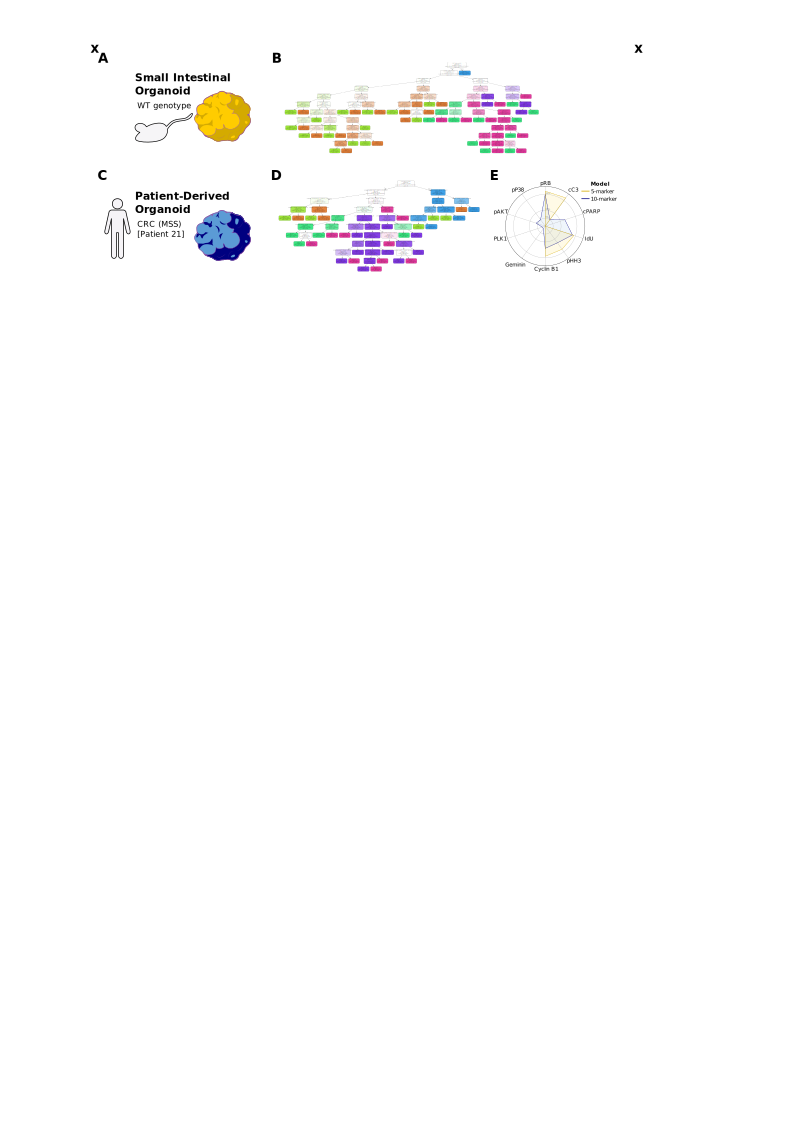
\includegraphics{02methods/figs/2CYTOF_trainRFclass.png}
    \caption{}
    \label{}
\end{figure}

\subsection{RF Classifier Models}


This classifier implementation was used to build two models distinguished by the features they use and the type of epithelial cells they were trained on. 

The simpler 5-marker model uses only 5 cell state markers and was trained using a balanced subset of cells from the Small Intestinal murine organoid time-course experiment in Qin et al. 2020 \cite{qin_cell-type-specific_2020}. This model uses the same exact antibody markers as those used by Qin et al. 2020 to label cell state via manual gates, namely: pRB [S807/S811], cleaved Caspase 3 [D175], IdU, Cyclin B1, and pHH3 [S28].

The more complex 10-marker model was trained using CRC Patient Derived Organoids. With an updated panel, the markers used in the latest models are a set of ten antibodies (the five markers from above plus cPARP [D214], pAKT [T308], pP38 [T180/Y182], Geminin, and PLK1) with targets specific to each of the six cell state classes (Apoptosis, G0, G1, S-phase, G2, and M-phase). The data used to train this model has been published in Ramos Zapatero \& Tong \emph{et al.}~\cite{zapatero_trellis_2023} and belongs to an untreated monoculture replicate of PDO21. 

Details on the markers used in the RF models, and the cell state they are associated with, can be found in Table \ref{tab:2rfmark}. 

\begin{table}
\centering
\begin{tabular}{| p{3.6cm} p{4.8cm} p{3.6cm} |}
    \hline
    \textbf{Marker} & \textbf{Specificity} & \textbf{Model} \\
    \hline\hline
    pRB [S807, S811] & Proliferating cells & 5-marker, 10-marker \\
    \hline
    pAKT [T308] & PTM in the mTOR pathway (proliferation) & 10-marker \\
    \hline
    pP38 [T180, Y182] & PTM promoting \textbeta-cat activation (proliferation) & 10-marker \\
    \hline
    pHH3 [S28] & M-phase & 5-marker, 10-marker \\
    \hline
    PLK1 & G2/M-phase transition & 10-marker \\
    \hline
    Cyclin B1 & G2 & 5-marker, 10-marker \\
    \hline
    IdU & S-phase & 5-marker, 10-marker \\
    \hline
    Geminin & Negative marker of G1. Expressed in S-phase, G2, and M-phase & 10-marker \\
    \hline
    cCaspase 3 [D175] & Apoptosis & 5-marker, 10-marker \\
    \hline
    cPARP [D214] & Apoptosis & 10-marker \\
    \hline
\end{tabular}
\caption{Table of Markers}
\label{tab:2rfmark}
\end{table}

    % Some of the results presented in this document correspond to an initial implementation of the RF algorithm that used only 5 different cell state markers: pRB [S807/S811], cleaved Caspase 3 [D175], IdU, Cyclin B1, and pHH3 [S28]. This 5-marker implementation was trained using a balanced subset of cells from SI LGR5 time-course experiment in Qin et al. 2020 \cite{qin_cell-type-specific_2020} (downsampled so that all six cell states would have the same number of cells, 5306). The trained model was then tested against datasets from the same publication; a simpler single-timepoint SI LGR5 culture, and a complex coculture of colonic organoids (with varying degrees of CRC mutations and TME complexity).
    % In contrast, the latest results use data acquired from Patient Derived Organoids of CRC patients. With an updated panel, the markers used in the latest models are a set of ten antibodies (the five markers from above plus cPARP [D214], pAKT [T308], pP38 [T180/Y182], Geminin, and PLK1) with targets specific to each of the six cell state classes (Apoptosis, G0, G1, S-phase, G2, and M-phase). This 10-marker model was trained on an untreated control condition replicate and testing is performed against a second set of replicates comprising a total of 5 conditions (plus an untreated control) treated with increasing concentration of the chemotherapeutic topoisomerase inhibitor SN-38.


    % \colorbox{yellow}{TRain a model and evaluate performance}
    % The script performs the following tasks:
    
    % Imports necessary libraries and modules.
    % Sets up input/output directories and creates necessary folders if they don't exist.
    % Asks for user input to provide information about the run.
    % Checks if the specified output directory already exists and exits the script if the run name has been used before.
    % Reads and processes the training data from a specified directory.
    % Balances the classes in the training data by downsampling if necessary.
    % Translates antibody markers in the training data.
    % Prepares the training and validation datasets for the random forest classifier.
    % Trains a random forest classifier and performs calibration on it.
    % Generates predictions and probabilities for the test data using the trained model.
    % Evaluates the performance of the model using various metrics such as classification reports, confusion matrices, and log loss.
    % Saves the trained model and outputs relevant plots and reports.
    
    % \colorbox{yellow}{Classify a dataset using a pre-trained model}
    % The script performs the following tasks:
    
    % Importing necessary libraries and modules: pandas, numpy, matplotlib.pyplot, os, sys, joblib, sklearn, and seaborn.
    % Importing custom functions from the "aux" module.
    % Setting up the folder structure for input and output data.
    % Defining the model to use for labeling cell states and loading the corresponding model file using joblib.
    % Prompting the user to provide information about the run and handling the input.
    % Checking if the input data is already labeled with cell states.
    % Reading the input data from the specified folder and storing it in a list.
    % Checking the features used in the model and translating the column names of the input data to match those features.
    % Handling data preprocessing steps such as filtering and normalizing.
    % Predicting cell states on the input data using the loaded model.
    % Adding the predicted labels to the original data frames and saving the results as CSV files.
    % Calculating and displaying prediction scores (accuracy, balanced accuracy, classification report, confusion matrix, F1 score) if the input data is labeled.
    % Saving the classification report and confusion matrix as files and plotting the confusion matrix.


\newpage
\section{scRNA-seq Data Analysis}

Work presented in this section has already been made public in Qin \& Cardoso Rodriguez et al. 2023 \cite{cardoso_rodriguez_single-cell_2023}. As a joint co-first authored paper, attribution is shared between Dr. Xiao Qin and myself. While I carried out all of the scRNA-seq Data Analysis presented in this Thesis, Dr. Xiao Qin was in charge of the murine colonic organoid culture system and data acquisition via both scRNA-seq and Mass Cytometry. The exact attribution for specific tasks is detailed in Qin \& Cardoso Rodriguez et al. 2023 \cite{cardoso_rodriguez_single-cell_2023}. 

Aiming to provide additional context, the section below on scRNA-seq data acquisition has been included despite Dr. Xiao Qin having carried-out the work.

% \subsection*{Wet Lab Data Generation}

% This work wasn't carried out by me and this should be made very clear. Instead of detailing it here, perhaps it would be best to reference the preprint/article once up?

% Generation of murine colonic organoid heterocellular cultures as shown in 


\subsection{Data Acquisition}

In brief, the organoid heterocellular culture system was dissociated into single-cells, FAC-Sorted for live cells, counted and fixed with methanol before scRNA-seq library preparation. For co-cultures, different cell-types were mixed at equal cell numbers prior to the fixation step. scRNA-seq libraries were generated with the 10X Genomics Chromium Next GEM Single Cell 3' Reagent Kits v3.1 (Dual Index) and sequenced with the Illumina NovaSeq 6000 System (2$\times$ 150 bp paired-end reads), aiming at 60,000 read pairs per cell and 2,000 cells per cell-type per sample.

\subsection{Data Processing}
% Raw scRNA-seq data was converted to FASTQ files and processed with the 10X Genomics Cell Ranger pipeline version 5.0.1. Sequencing reads were aligned to a custom GRCm38 reference genome containing the sequences of \hl{\textit{DsRed} and \textit{eGFP}} transgenes present in fibroblasts and organoids respectively.

The Illumina NovaSeq binary base call (BCL) outuput sequence files were converted to FASTQ files and processed with the 10X Genomics Cell Ranger pipeline version 5.0.1 \cite{10x_genomics_what_nodate}, which provides with a convenient wrapper for Illumina's bcl2fastq tool \cite{illumina_bcl2fastq_nodate}, \texttt{cellranger mkfastq}. Prior to alignment, a custom murine GRCm38-based reference genome was generated using the STAR aligner \cite{dobin_star_2013} wrapper \texttt{cellranger mkref}. By adding the sequences for \textit{DsRed} and \textit{eGFP} transgenes present in fibroblasts and organoids respectively, cell type discrimination based on exogenous transcripts was facilitated. Then, alignment of the FASTQ files against this custom reference was performed using the \texttt{cellranger count} pipeline, generating both unfiltered and pre-filtered feature-barcode matrices.

The resulting feature-barcode matrices were analysed with the R package \textit{Seurat} version 4.0.4 \cite{hao_integrated_2021}. 
The analysis pipeline encompasses quality control, data normalisation, data integration, dimensionality reduction, cell clustering, and analysis of differential gene expression. 
Genes found in less than 4 cells were removed during QC and only cells with at least 600 unique genes identified were kept for downstream analysis. The total number of detected reads per cell typically ranged from 1,200 to 80,000, with the actual values manually determined based on dataset sequencing depth and cell-type composition. 
Cell type composition was considered as the macrophages were observed to be captured less efficiently than fibroblast or epithelial cells.
For the integrated epithelial object in used throughout the analysis, an additional filtering step was performed to remove cells with undetectable expression for any one of the \emph{bona fide} pan-epithelial genes \textit{Epcam}, \textit{Krt8}, \textit{Krt18}, \textit{Krt19}, \textit{Cldn7}. 
Doublet/multiplet filtering was explored using the scDblFinder package \cite{germain_doublet_2022}, which has been designed to find heterotypic doublets such as those that could be present in co-culture conditions. However, after the QC pipeline outlined above, the low number and homogeneous distribution on 2D embeddings of the putative doublets was not deemed convincing enough to warrant their removal.

The Seurat object, much like its SCE counterparts in R or AnnData objects in Python, contains multiple layers where different \(barcode X feature\) matrices can be stored. This is so it can accommodate for different normalisation methods and for tools that expect raw or processed gene expression values. 

Gene expression values were normalised for total counts, multiplied by a scale factor of  \(1\cdot10^4\), and the expression values log transformed as \(X = \log_2 (X+1)\). The resulting normalised count matrix was used for methods that rely on the explicit comparison or visualisation of gene expression.

An alternative normalisation approach was used as described in Hafemeister \& Satija 2019 \cite{hafemeister_normalization_2019}. Named sctransform (SCT) this method models both biological and technical variation using the Pearson residuals from a regularised negative bionamial regression. The nature of this model allows for certain signals to be regressed out, such as the percentage of mitochondrial transcripts over the total reads in a cell, or for differences between cycling cells in different phase of the cell cycle. I computed SCT normalised count matrices with 6,000 features and regressed out mithoncondrial content and differences between cell cycle phases.

Cell Cycle scores were computed using the CellCycleScoring function from Seurat (a wrapper for AddModuleScore) and a curated list of cell cycle genes shown in \ref{tab:cycle}. By comparing how well a cell matches the G2 and M-phase signature, versus a G1 and S-phase signature, cells could be classed into Dividing cells (Mitosis and G2), Cycling (G1 and Synthesis), and Other (cells with low scores for both signatures, most likely outside of the cell cycle). Differences between the Dividing and Cycling groups were also regressed out when computing the SCT normalised count expression data, as it was deemed that intra-cycle differences were not central to the biological system being studied. This computation of cell cycle scores used a custom table of cell cycle genes shown in Sup. Table \ref{tab:cycle}.

Throughout the study, steps that relied on building a k-NN graph or low-dimensional representation of the data use either the SCT normalised data or the SCT-derived integrated representation (see section below).

\subsection{Integration}

Dataset integration was performed using Seurat's reciprocal PCA (RPCA) implementation \cite{hao_integrated_2021} as it has been optimised to handle large datasets. RPCA works by projecting the individual datasets into an other's PCA space to identify cellular anchors with shared neighbourhoods across projections. The integration itself is described in Stuart et al. 2019 \cite{stuart_integrative_2019}, so that new expression matrices in the integrated space are computed based on the difference of expression matrices between anchor cells. Inherently a pairwise process, integration of multiple datasets is done iteratively by pairs accordings to their pairwise distances. In this work I used the SCT normalised data as the feature space to be integrated and ran default parameters but for a k.anchor of 12.
The integrated object presented in Figure \ref{fig:4exp} was computed using all cells from the 20 conditions shown in the figure, resulting in a total of 58,726 cells with the integrated assay limited to 2,000 genes. The integrated object first presented in Figure \ref{fig:4intepi} and found elsewhere across this work was computed using just the epithelial cells from all conditions, resulting in an object with 29,452 cells limited to 4,000 genes. The respective integrated feature spaces were stored within the integrated assay of the Seurat object.

The integration pipeline with anchors found via Canonical Correlation Analysis was also tested, but as described in the literature, it was found to be less computationally efficient and appeared to smooth out and erase too much biological signal \cite{stuart_integrative_2019}. 
% \colorbox{yellow}{(small figure comparing umap from cca VS rpca, coloured by crctme label)}.

When handling the aggregated data from multiple CRC patient cohorts presented in Joanito et \emph{al.}~\cite{joanito_single-cell_2022}, where data integration was performed mostly for visualisation purposes, the methods described above struggled to handle the high number of cells present (>40,000 cells). As one of the goals of this data integration approach was to compare our murine organoids with human samples, I used scVI \cite{lopez_deep_2018}, a Variational AutoEncoder approach that can be GPU-accelerated and performs well on inter-species integration tasks \cite{song_benchmarking_2023}. Part of a broader family of PyTorch-based methods for analysing single-cell omics data \cite{gayoso_python_2022}, scVI learns a low dimensional latent space that can be used to compute 2-dimensional embeddings of the data. Able to account for multiple quantitative and categorical confounding variables, this method can also handle the projection of query datasets onto an integrated reference.
Cross-species data integration was thus achieved by generating an integrated reference from the human CRC datasets (filtered to the top 6,000 most variable genes) and projecting into it a humanised version of the mouse organoid data from Figure \ref{fig:4intepi}. The integrated human reference was built using unique patient identifiers as the batch key and controlling for the percentage of mitochondrial reads in a cell. The resulting latent space was embedded into 30 dimensions. Humanisation of the mouse count matrix was accomplished via the mousipy package \cite{peidli_mousipy_2023}, which facilitates the handling of mouse genes with multiple human orthologues. Untransformed count data was used for the scVI workflow. 

\subsection{Dimensionality Reduction}

To generate the EMD PCA plots shown in Figure \ref{fig:4exp}C I used the normalised gene expression data of all cells of a particular cell type (organoids, fibroblasts, or macrophages) stored within the RNA assay of the integrated Seurat object from Figure \ref{fig:4exp}B. EMD scores for the top 6,000 variable genes of each condition were computed with CyGNAL \cite{ferran_cardoso_tape-labcygnal_2021} using the relevant control condition for each cell type: WT monoculture for epithelial organoids, fibroblast monoculture for fibroblast cells, and macrophage monoculture for macrophage cells. The collection of gene-specific EMD scores for each condition was then used to compute a PCA space where each dot represent a whole condition.

The standard pipeline for generating single-cell embeddings consisted of computing a set of 50 to 100 principal components (PC) from a normalised count matrix, from which 2-dimensional PHATE embeddings were generated with default parameters. PHATE was chosen as the default DR method for visualisation due to its capacity to capture the global structure in biological settings with important developmental trajectories \cite{moon_visualizing_2019}. In the context of integrated datasets via scVI, the 30-dimensional latent space was used to generate the PHATE embeddings. 
This mid-dimensional PCA space was also used to compute most of the \emph{k}-NN cell-cell graphs used throughout the study. 


\subsection{Unsupervised Clustering and Differential Expression}

Cell clustering was computed using the Leiden algorithm on the \emph{k}-NN graph generated from the integrated epithelial dataset (first 48 PCs), at a series of resolutions ranging from 0.2 to 0.8. The final cluster annotations were retrospectively defined by curated cell-type marker expression (Figure \ref{fig:4intepi}C), inter-cluster relationships on a multi-resolution clustering tree \cite{zappia_clustering_2018}, and cross-condition differential abundance behaviours (Figure \ref{fig:4da}). Cells from outlier clusters (totalling less than 1\% of all epithelial cells) were excluded from the downstream analysis (Figure \ref{fig:4intepi}A).

Differentially Expressed (DE) genes between clusters, conditions, and cell neighbourhoods were identified using Wilcoxon rank-sum tests as implemented in Seurat's \textit{FindAllMarkers} and \textit{FindMarkers} functions. The Wilcoxon rank-sum test is commonly used in the field of scRNA-seq as it \colorbox{yellow}{.... Non parametric, assumption being that samples being compared are independent}. DE results in the form of log transformed Fold Changes in gene expression and p-values adjusted for multiplicity of tests.

Heatmaps of selected marker genes were generated with the R package \textit{ComplexHeatmap} \cite{gu_complex_2016}. Gene lists in Figures \ref{fig:4de} were curated from previously reported markers for colonic epithelial subpopulations and DE genes detected between epithelial clusters, conditions, and DA neighbourhoods within this study. Gene lists in Figures \ref{sfig:deepibyfib}, \ref{sfig:defib}, and \ref{sfig:demac} represent DE genes between conditions.

\subsection{Differential Abundance}

Differentially abundant (DA) cell neighbourhoods were identified using the R package \textit{MiloR} \cite{dann_differential_2022}. Milo works by constructing cellular neighbourhoods on a \emph{k}-NN graph. These neighbourhoods can overlap with one another, for cells may belong to multiple neighbourhoods at once, and act as the basis of Milo's compositional analysis. By comparing the composition of these neighbourhoods in terms of a categorical variable of interest (condition), Milo assigns them an enrichment score (log Fold Change) according to the relative abundace of cells from the query or control condition. Significance and regression out of technical and unwanted biological variables is achieved though a Generalised Linear Model via the mature edgeR package \cite{robinson_edger_2010}, and using the SpatialFDR metric (first described in Lun et al. 2017 \cite{lun_testing_2017}).
DA analysis thus allows for the detection of enrichment and depletion of epithelial cell states caused by microenvironmental and/or genotypical perturbations in the organoid system. 

For the analysis shown in Figure \ref{fig:4da}A-B I set the DA test threshold at 5\% SpatialFDR. In the context of fibroblast regulation of the colonic epithelia, given that CD34\textsuperscript{hi} and CD34\textsuperscript{lo} fibroblasts do not differentially regulate epithelial cells (Figure \ref{sfig:deepibyfib}), all samples of WT organoid+fibroblast co-cultures were grouped and considered replicates of the query condition regardless of the CD34 status of the fibroblasts. AK and AKP organoid monocultures were also grouped due to their similar DE and DA behaviour (Figures \ref{fig:4de}, \ref{fig:4da}C).
The DA overview dot plot in Figure \ref{fig:4da}C was generated by comparing the 17 conditions against the WT monoculture control (2$\times$ replicates). Size of the dots represents the number of neighbourhoods associated with a particular combination of cluster and conditions, while dot colour shows the median log Fold Change value for those neighbourhoods. Absence of replicates in this approach results in a lack of relevance for the SpatialFDR statistic, and the control condition (1st row) was populated with empty values for visualisation purposes. 

The \emph{k}-NN graphs used by Milo where constructed as detailed in the section above.

\subsection{Signature Score Correlations}

By gathering more than 50 gene lists from the literature that describe key signalling pathways and stem-related gut epithelia states~\cite{ayyaz_single-cell_2019, vasquez_molecular_2022, alvarez-varela_mex3a_2022, mustata_identification_2013,  yui_yaptaz-dependent_2018, munoz_lgr5_2012, li_reference_2017, han_lineage_2020, merlos-suarez_intestinal_2011, dalerba_single-cell_2011, pelka_spatially_2021, gregorieff_yap-dependent_2015, canellas-socias_metastatic_2022, wang_comprehensive_2018, mourao_lineage_2019, barriga_mex3a_2017, bues_deterministic_2022, morral_zonation_2020}, I could put the results of this study in context with a broader corpus of works in varied settings; such as human data, cancer, or tissue repair processes.
Gene lists for different intestinal stem cell-states were compiled from public datasets, together with transcriptional targets of key signalling pathways associated with the different stem cell-states. Gene identifiers where transformed to murine Gene Symbols (to be compared with the features in the sequencing dataset) by querying BioMart \cite{smedley_biomart_2009}. Metadata for the resulting compiled list can be found in Sup. Table \ref{tab:SignMD}.

These gene lists were compared with the curated gene signatures for proliferation, CSC, revCSC, and proCSC cell-states in Figure \ref{fig:4de}, as well as the top DE genes for each stem cluster (adjusted p-value < 0.01, log2FC > 0.25, top 24 genes with the greatest positive log2FC values). \textit{UCell} scores for each gene set were calculated using Log-normalised gene expression values and z-scored to allow cross-signature comparison.

The \textit{UCell} \cite{andreatta_ucell_2021} method was used to generate the correlation matrix between gene signatures in existing literature and cell clusters identified within this study (Figure \ref{fig:4sign}A). UCell uses the Wilcoxon rank-sum test, also known as Mann-Whitney U, and a matrix of ranked genes (by expression) for each cell in the dataset. Given a list of genes, UCell can then score how well each cell matches their expression. Unlike Seurat's AddModuleScore function (and it's re-implementaion in scanpy), the resulting scores are not normalised against a control gene set, making UCell scores impervious to dataset composition. 

Pearson correlations were computed between the relevant scores (i.e. those whose context refers to the stem compartment or key signalling pathways) on all cells of stem and TA clusters and then visualised as a heatmap-like correlation matrix with the corrplot package \cite{wei_r_2021}. Signatures that did not have a SD deviation of scores greater than 0.2 across the cells where excluded from the analysis (as they would equally mark all states present in the dataset), and matrix entries where populated for significant correlations (confidence level of 0.95). Finally, the matrix was ordered and grouped via complete linkage hierarchical clustering (k=3). 


\subsection{Signalling Entropy and Pluripotency}

Leveraging the concept that cells with a higher potency should have a higher signalling entropy \cite{teschendorff_signalling_2014}, the pluripotency values for epithelial cells across the different clusters were estimated using the R package \textit{SCENT} \cite{teschendorff_single-cell_2017}. 
Signalling entropy scores for all epithelial cells in Figure \ref{fig:4dyn}A were determined via the CCAT approximation method, which computes a Pearson correlation between a cell's transcriptome and the interactome as defined by the built-in \textit{net17Jan16} Protein-Protein interaction network (derived from the Pathway Commons database). As the interaction network is annotated with NCBI gene IDs, BioMart was used to translate them to MGI gene symbols.

Being a method that is completely independent of any cell metadata, like clusters or conditions, the resulting vector of CCAT scores was added as a new metadata column to the sequencing dataset object and used to quantify pluripotency changes in Figure \ref{fig:4dyn}B and as one of the components of the Valley-Ridge score (Chapter \ref{05vr}).


\subsection{RNA Velocity and Cellular Dynamics}

For RNA velocity analysis, loom files were generated from Cell Ranger's output using the command line interface tool \textit{velocyto} \cite{la_manno_rna_2018}. The murine GRCm38 reference was used, with the GRCm38/mm10 repeat mask assembly and the RepeatMasker track. RNA velocity was analysed with the Python package \textit{scVelo} \cite{bergen_generalizing_2020} using close to default parameters. Metadata and PHATE embedding coordinates were exported from the relevant Seurat objects to filter and annotate AnnData objects generated from the loom files made by velocyto. Moments for the velocity estimation were calculated using the first 50 PCs and 30 neighbours from the AnnData objects. RNA velocities were computed with the \textit{recover\_dynamics} function using the dynamical model of transcriptional dynamics with default parameters. The velocity stream embedding (Figure \ref{fig:4dyn}A) was computed using the integrated object containing epithelial cells from all conditions. The RNA velocity vector lengths, an estimate of a cell's rate of transcriptional change, were computed using cells solely from the 4 conditions shown in Figure \ref{fig:4dyn}C. The quantitative comparison in Figure \ref{fig:4dyn}D was performed using the Games-Howell pairwise test wrapper from the R package \textit{statsExpressions} \cite{patil_statsexpressions_2021}. All conditions were compared against the WT monoculture control and all \textit{p}-values have been corrected for multiplicity with the Holm method.

Initial and terminal macrostates where determined using CellRank \cite{lange_cellrank_2022}, which leverages RNA velocity information to describe cellular dynamics. The matrix of cell-cell transition probabilities was constructed as a weighted combination of the transition matrix based on velocity directions (through the VelocityKernel class, weight of 0.8) and a symmetric transcriptional similarity matrix (through the ConnectivityKernel class, weight of 0.2). Macrostates, and their transition probabilities, were computed using the built-in Generalised Perron Cluster-Cluster Analysis (GPCA) estimator. To find initial macrostates, inverse velocity vectors are used to assemble the transition matrix by setting the backward argument to \texttt{True} when computing the VelocityKernel component. Directed PAGA plots \cite{wolf_paga_2019, lange_cellrank_2022} were computed so that epithelial clusters are represented as nodes shown on top of a low dimensional embedding and are connected by directed edges whose thickness represents local velocity flows.

\subsection{Cell-Cell Communication Analysis}

Cell-cell communication inference was performed using the R package CellChat \cite{jin_inference_2021}, where stromal-epithelial signalling was analysed across 4 different organoid genotypes (WT, A, AK, and AKP). CellChat uses a database of interactions between ligands, receptors, and cofactors. 
Using cluster annotations and the gene expression matrix, interaction probabilities can be inferred between the different populations using a permutation-based approach. The inferred interactions can the be grouped at the pathway level, and functional analysis of the clusters can be infered via network analysis methods. 

Epithelial cells were annotated with the clusters previously identified (Figure \ref{fig:4intepi}A), while the fibroblasts were grouped as a single cluster. A merged CellChat object was generated to compare relative communication probability of fibroblast-to-epithelia signalling across the genotypes. Significant ligand-receptor pairs were identified based on CellChat's murine cell communication database. Plots displaying aggregate outgoing and incoming communication probability (Figure \ref{fig:4cc}A) were generated with the \textit{netAnalysis\_signalingRole\_scatter} function. Detected communication at the pathway and interaction level was accessed with the \textit{subsetCommunication} function and probabilities were z-score normalised to allow for cross-pathway or cross-interaction comparison. The results were visualised with ComplexHeatmap in Figure \ref{fig:4cc}B, the rows of which were manually ordered based on hierarchical clustering and grouped based on the nature of the interaction. Gene expression of the ligand-receptor pairs identified above was visualised using Seurat's \textit{Dotplot} function in Figure \ref{fig:4cc}C. \textit{UCell} scores for ligand and receptor genes were calculated for fibroblasts and epithelial cells respectively and quantified in Figure \ref{fig:4cc}D. Games-Howell pairwise test was performed using the R package \textit{statsExpressions} and all \textit{p}-values have been corrected for multiplicity with the Holm method.


\section{VR Score and Data-Driven Waddington-like Landscapes}

Work presented in this section has already been made public in Qin \& Cardoso Rodriguez et al. 2023 \cite{cardoso_rodriguez_single-cell_2023}. I am the author behind the Valley-Ridge (VR) score design and implementation, including the python-based renders of the data-driven Waddington-like landscapes. 

Dr. Jeroen Claus however, kindly rendered the landscapes shown in Figure 6 of Qin \& Cardoso Rodriguez et al. using professional rendering software. The exact attribution for specific tasks is detailed in the manuscript \cite{cardoso_rodriguez_single-cell_2023}.

\subsection{VR Score Computation}

The VR score is cell-based metric defined as the weighted sum of the Valley and the Ridge components (Figure \ref{fig:5score}):
\[VR = 0.9V+0.1R\]
where V is the Valley component and R the Ridge component.

The Valley component is computed as \(V = med(CCAT)_{s,c}\) for each combination of sample (\(s\)) and cluster (\(c\)). 

Let $u$ be scaled representation of the velocity vector length for each cell ($\frac{1}{|v|}$), and $d$ be the scaled median $L^1$ distance of each cell to all other cells from the same cluster. $d$ acts a cell centrality metric computed on a \emph{k}-NN graph of a cluster PHATE embedding, followed by the calculation of a shortest distance matrix (using the graphtool software \cite{peixoto_graph-tool_2014}) whereby cells with the lowest median distance would be at a cluster's centre whilst those with the highest distance would be at the cluster periphery. Outliers with a distance over $Q_{99}$ were set to the median distance. 
To allow for inter-cluster comparisons, $d$ was scaled for each cluster to the (0,1) range with sklearn's MinMaxScaler() \cite{pedregosa_scikit-learn_2011}, whereas $u$ was scaled at a dataset level using the same function.
The Ridge component is then computed per each cell as $R = med(u)_{s,c} \cdot d$. 

% The Valley component equals the median CCAT value of each sample-cluster combination
% To calculate the Ridge component, the inverse of the velocities was first computed and scaled to a range between 0 and 1. A cell centrality distance was then calculated for cells in each cluster by first building a \emph{k}-NN graph of a cluster's cells from the PHATE embeddings (Table S2), followed by the calculation of a distance matrix . The median distance for each cell to all other cells was then calculated, whereby cells with the lowest distance would be at a cluster's centre whilst those with the highest distance would be at the cluster periphery. To allow inter-cluster comparisons, outliers with a distance over $Q_{99}$ were set to the median distance value before scaling to (0,1). Finally, the Ridge component was computed per sample-cluster as the product of the median scaled inverse velocities and the cell's scaled centrality distance (Figure \ref{suppfig:figs7}A).

This definition of the VR score allows the CCAT-based Valley component to be the driving force for sculpting the landscape and the velocity-driven Ridge component to predominately define local features at the boundaries between clusters, producing a tarn-like effect symbolising a state of trapped cells in cluster whose cells present low velocity vector lengths. In principle, any other dimensionality reduction technique can be used in place of PHATE \cite{chen_single-cell_2019}, and the Valley/Ridge component can be computed using other metrics underpinning pluripotency and cell-fate transition. The Ridge component can also be calculated with a distance-free approach such as \textalpha-shapes \cite{bellock_bellockkalphashape_2021}. Finally, the VR scores could be computed on a per cell or neighbourhood basis, which would increase landscape resolution and liberate the method from constraints of cluster definitions (at the expense of increased noise).

\subsection{VR Landscape Projection}

To generate the Waddington-like landscapes in Figure \ref{fig:5score}B, I combine the ability of PHATE to capture the global structure of single-cell data with the VR score.

Waddington-like landscapes can be visualised directly in Python (Figure \ref{fig:2land}. Briefly, a low dimensional 34x30 mesh grid was generated from the PHATE embeddings, and a 3D surface was rendered by projecting VR scores onto the grid using the radial basis function interpolation from scipy \cite{virtanen_scipy_2020} (Table S2). The surface of the landscape was coloured by VR scores and a scatter plot was overlaid where the elevation of each cell was defined as the weighted sum of its VR score (weight = 0.9), CCAT value (weight = 0.1), and a constant factor of 0.012 (weight = 1). This added a level of controlled noise to the scatter plot while ensuring most cells remain above the interpolated surface.

\begin{figure}
    \centering
    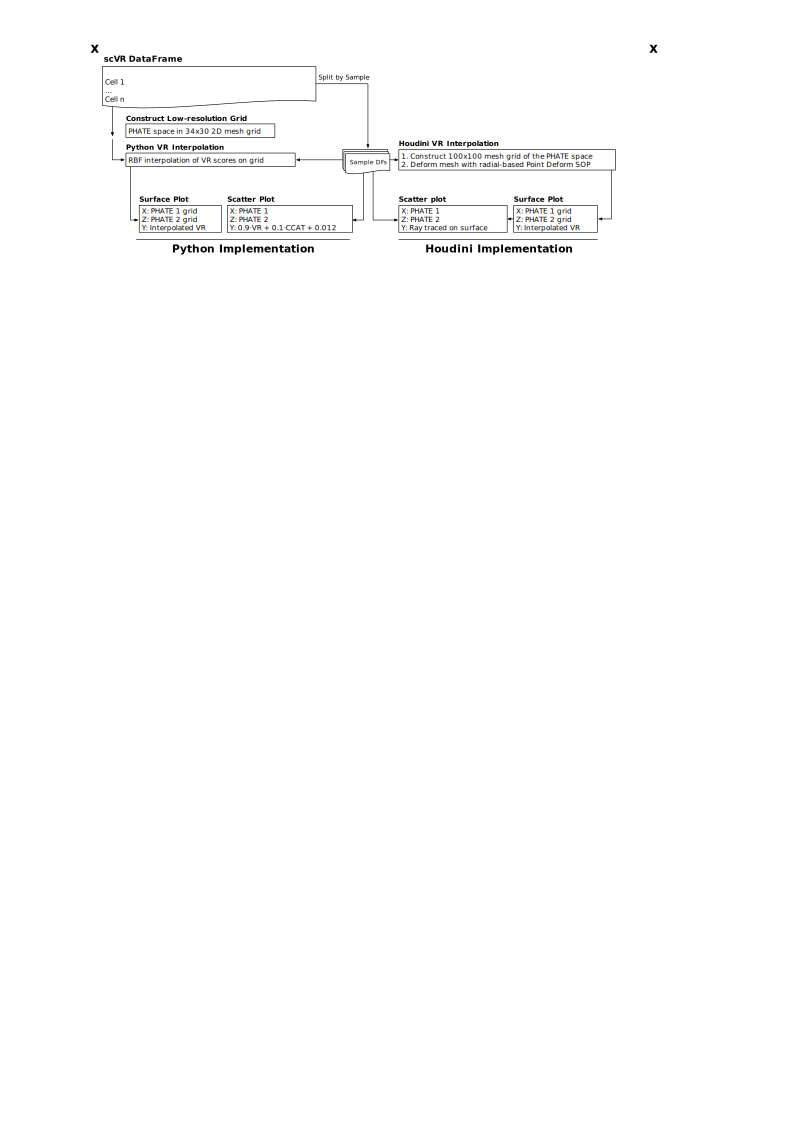
\includegraphics{02methods/figs/2VR_Landscape.png}
    \caption{Generation of Waddington-like Landscapes from scRNA-seq Data}
    \label{fig:2land}
\end{figure}

Finally, external software can also be used to render the data-driven landscapes, as shown in Qin \& Cardoso Rodriguez et al. 2023 where we used the 3D rendering programmes SideFX Houdini and Maxon Redshift (Figure \ref{fig:2land}).


% \subsection{Tool packaging/deployment with jupyter notebooks and nbdev}


% \colorbox{yellow}{Current notebook explanation}

% 1. Import necessary libraries: matplotlib, plotly, pandas, numpy, graphtools, scipy, sklearn
% 2. Define a function `compute_distdeg` that takes several arguments including an input dataframe, a column to split by, a list of columns to use for computation, and several optional arguments such as knn, distance metric, scale and plot options.
% 3. Within the `compute_distdeg` function:
%     a. Initialize an empty output dataframe with specified columns
%     b. Loop over unique values in the `split_by` column of the input dataframe
%     c. For each unique value:
%         i. Subset the input dataframe to only include rows where the `split_by` column equals the current unique value
%         ii. Create a graph using the subsetted dataframe and specified knn and distance metric
%         iii. Compute distances using shortest path on the graph
%         iv. Compute median distance to all cells for all cells
%         v. Add distance and degree columns to the subsetted dataframe
%         vi. Optionally remove outliers by replacing distant outliers with median value
%         vii. Optionally scale distance and degree columns
%         viii. Optionally plot cluster cells on phate and color by distance from centroid
%         ix. Concatenate subsetted dataframe with output dataframe
%     d. Return output dataframe
% 4. Load cell data from a csv file into a pandas DataFrame
% 5. Call `compute_distdeg` function on cell data with specified arguments and store result in a new DataFrame
% 6. Merge result with original cell data DataFrame on specified columns
% 7. Scale velocity length for all cells in cell data DataFrame using MinMaxScaler from sklearn.
% 8. Display final cell data DataFrame.

\newpage
\section{Knowledge Graphs for Cell Communications}

\subsection{Sources and Assembly}

Interaction information found in cell communication databases can be parsed and formatted as a \acrfull{kg}. To assemble the custom Ligand-Receptor-Target \acrshort{kg} (LRT-KG) I accessed the CellChat~\cite{sqjin_sqjincellchat_2021} and NicheNet~\cite{browaeys_nichenet_2020} databases. Ligands and receptors were gathered from both databases, whereas \acrfull{tf} target genes were extracted from NicheNet's. Formatted as lists of human gene symbols, the three categories (ligands, receptors, and targets) were pruned to ensure there was no overlap between them, simplifying the \acrshort{kg} and enhancing it's hierarchical nature. 

The \acrshort{kg} was assembled as a table of relational triplet entries wherein a \emph{head} node interacts with a \emph{tail} node via a \emph{relation} edge. This relational information was obtained from the Reactome database of curated pathways~\cite{gillespie_reactome_2022}. Assembly of the \acrshort{kg} was thus achieved by iterating through all possible \emph{head} and \emph{head} combinations and creating a \emph{relation} between them if both were found to belong to the same pathway level in Reactome's second level of pathway hierarchies.

The \emph{de novo} assembled custom LRT-KG was compared with the popular curated repository of cellular interaction knowledge OmniPath~\cite{turei_integrated_2021}, which contains almost four times the amount of nodes present in the LRT-KG but with a similar number of relations, resulting in a slightly lowered average degree (Table \ref{tab:2kg}). By processing the OmniPath database as detailed above and incorporating the pathway information from Reactome we observe how the number of distinct pathways present is also higher than in the LRT-KG, with 33 and 23 unique pathways respectively (Table \ref{tab:2kg}).

Hierarchy of the assembled graphs was computed using my python package \emph{pykrack} (\url{pypi.org/project/pykrack/}), which computes the Krackhardt hierarchy score for a given directed graph (see Appendix \ref{appendix:pykrack} for more details). The OmniPath graph is highly hierarchical before and after processing, and the LRT-KG hierarchical design results in a completely hierarchical tree-like structure (Table \ref{tab:2kg}).

\begingroup %Spacing only for this table
\renewcommand{\arraystretch}{1.2} % Default value: 1
    \begin{table}
    \centering
        \begin{tabular}{| p{1.8cm} p{1.8cm} p{1.8cm} p{1.8cm} p{1.8cm} p{1.8cm} |}
            \hline
            \textbf{Graph} & \textbf{Nodes} & \textbf{Edges} & \textbf{Pathways} & $\overline{\textbf{Degree}}$ & \textbf{Hierarchy} \\
            \hline\hline
            LRT & 2507 & 97054 & 23 & 77.43 & 1 \\
            \hline
            Omnipath & 9248 & 92262 & \textit{NA} & 19.95 & 0.82 \\
            \hline
            Omnipath (processed) & 9248 & 94836 & 33 & 20.51 & 0.78 \\
            \hline
        \end{tabular}
    \caption{Knowledge graph characteristics. Pathways is number of identified pathways from reactome. 81343/94836 of omnipath relations do not have direct match as same level pathway in reactome.}
    \label{tab:2kg}
    \end{table}
\endgroup

\subsection{Embedding the Knowledge Graph}

The table of relational triplets was then used to generate a\acrshort{kg} using the MultiDiGraph() function from the NetworkX package~\cite{hagberg_exploring_2008}, wherein multiple types of edges (\emph{relations}) connect nodes in a directed manner. 

The resulting directed \acrshort{kg} was then embedded into a lower 50-dimensional space using the TransR \acrshort{kg} embedding algorithm~\cite{zhang_transr_2021} as implemented in the PyKEEN package~\cite{ali_pykeen_2021}. TransR is a knowledge graph embedding approach derived from the mature TransE algorithm~\cite{bordes_translating_2013} that better encodes complex relational information. 

The embedding space was learnt on GPU compute using an 80:10:10 train, test, and validation split and otherwise default parameters.
To visualise the embedding the 50-dimensional space was embedded using PHATE (Figure \ref{fig:6embed}), or projected as a graph whose layout was determined via the Fruchterman-Reingold force-directed algorithm as implemented in NetworkX~\cite{fruchterman_graph_1991}.
Metadata was then added to the node-based embedding based on the presence of the gene symbols as ligands, receptors or \acrshort{tf} targets in the cell communication databases discussed above (Figure \ref{fig:6embed}A). Furthermore, pathway-level metadata from Reactome was also used to check for the presence of genes in each of the Reactome pathways (Figure \ref{fig:6embed}B).


\subsection{Wavelet Transform and Data Projection}

Via data projection I can then evaluate \emph{omic} profiles of cells as signals on a \emph{k}-NN graph derived from the \acrshort{kg} embedding. First the \emph{k}-NN graph is computed using the sklearn package~\cite{pedregosa_scikit-learn_2011} (n\_neighbors = 5). Then, on each of the nodes of the graph a wavelet bank is centred at and diffused at \(J\) scales, resulting on a flattened \(node X wavelets\) matrix; wherein nodes equal the number of genes in the \acrshort{kg}, and the wavelet bank equals genes times the scale parameter \(J\) (with all data shown using \(J = 4\)). A high-level overview of this process is presented in Figure \ref{fig:2wav}, where a single diffusion wavelet is shown centred around a particular node of the Stanford bunny graph~\cite{turk_zippered_1994} (Figure \ref{fig:2wav}A). A bank of wavelets at four scales (\(J = 4\)) is computed for the different nodes of the graph (Figure \ref{fig:2wav}B). 

This wavelet computation is based on a python script kindly provided by Aarthi Venkat from Prof. Smita Krishnaswamy's lab at Yale University (Table \ref{tab:wavpy}), which implements the wavelet definition from Coifman \& Maggioni~\cite{coifman_diffusion_2006} wherein a diffusion wavelet transform is the difference between two scales of lazy diffusion on a graph.
github
     % In order to extend this construction to graphs, we define graph wavelets as the difference between lazy random walks that have propagated at different time scales, which mimics classical wavelet constructions found in Meyer (1993) and more recent constructions found in Coifman & Maggioni (2006)

\begin{figure}
    \centering
    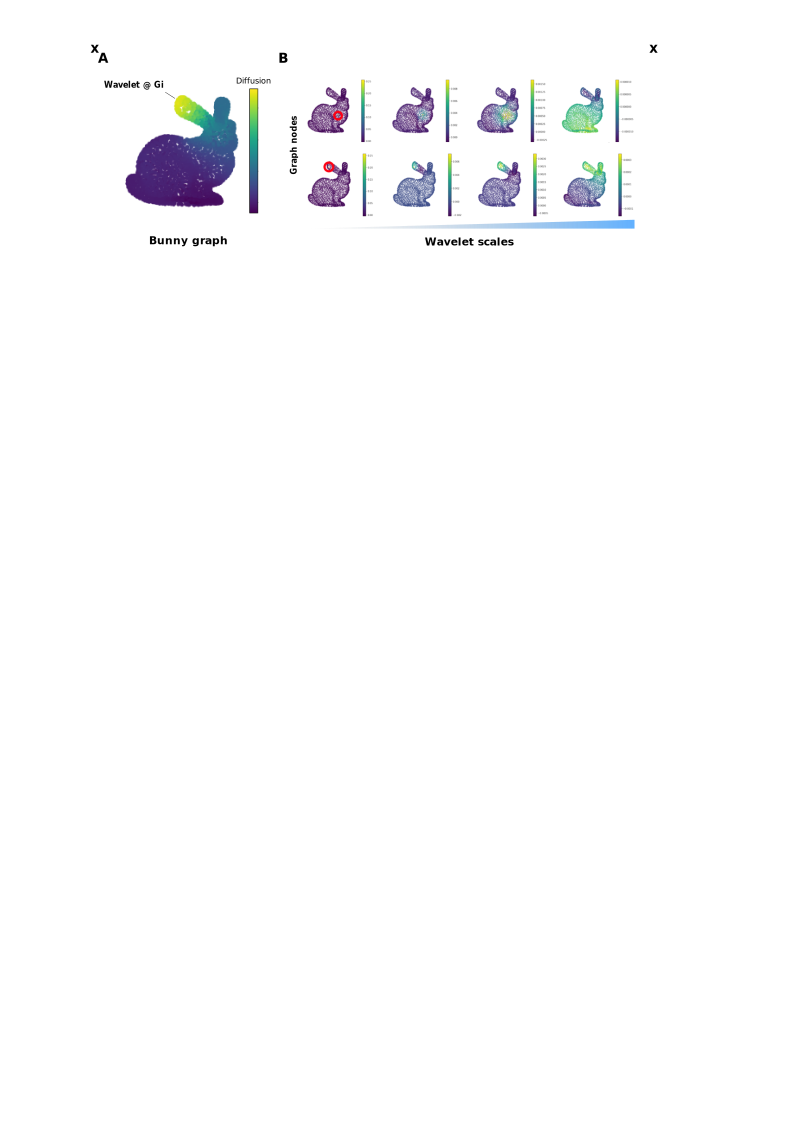
\includegraphics{02methods/figs/2KG_wav.png}
    \caption{}
    \label{fig:2wav}
\end{figure}

To generate the projected \(cell X wavelets\) matrix I compute the dot product between the \(node X wavelets\) matrix and the \(cell X feature\) count matrix with the numpy package~\cite{harris_array_2020}(Figure \ref{fig:6project}B).

A relatively high dimensional space, PCA is applied to the projected matrix and then a \emph{k}-NN graph and subsequent PHATE embedding are computed. The PHATE embedding serves as a useful non-quantitative way to compare the projected data with the original count matrix-based embedding (Figure \ref{fig:6project}).
The projected \emph{k}-NN graph can be used to quantitatively compare and benchmark the method against a \emph{k}-NN computed directly from the \(cell X feature\) count matrix (Figure \ref{fig:6bench}. Distances on the \emph{k}-NN graphs were computed using the shortest\_path() function from the graphtools package (\url{github.com/KrishnaswamyLab/graphtools}) and then aggregated at the cluster level by computing the mean distances from and to each pair of cell clusters (Figure \ref{fig:6bench}). To compare these inter-cluster distances between the gene expression and LRT-KG projection spaces (Tables \ref{tab:kgdistge} and \ref{tab:kgdistlrt}), the distance matrices were scaled to (0,1) range using the MinMaxScaler() function from sklearn and substracted to generate a matrix of distance differences (Figure \ref{fig:6bench}B). Pearson correlation between the two unscaled distances for each cluster-pair combination was computed with the scipy package (Figure \ref{fig:6bench}C), and so was the correlation between the distances and the aggregate communication probability score for each cluster pair as defined by CellChat (Figure \ref{fig:6bench}D). 


% \subsection*{Emebdding LR pairs to recovr info on fucntional communication}
% ALternative approach goes here. Run current notebook version and get results with out data so I can at least set on a draft method approach


\section{FAIR Spirit and Reproduceability}

Data and code are FAIR:

* Findable
* Accessible
* Interoperable
* Reusable

The code for CyGNAL can be found in the group’s GitHub repository at  https://github.com/TAPE-Lab/CyGNAL and remains under continued development. In addition to the main steps already presented, there are also a set of utility scripts that can be used for performing common dataset manipulations; such as downsampling, concatenation, and format conversion. In Sup. Figure 1 a detailed diagram depicting CyGNAL’s steps is shown.








        % \lstset{frameround=fttt,language=Python,numbers=left,breaklines=true}
        
        % Test the text. Now with \texttt{cobra.flux\textunderscore analysis}!
        
        % \begin{spacing}{1.5}
        % \begin{lstlisting}[caption={Pseudocode snippet for \texttt{1-data\textunderscore preprocess.py}}, breaklines=true,basewidth=6pt,frame=single,language=Python, numbers=left, prebreak=**, postbreak=**, label={lst:code}]
        % def run_meteor(model_path, constraints_path, **options):
        %   # Load in the model
        % 	model = cobra.io.read_sbml_model(model_path)
        %   # Load and apply the options
        % 	options = options.get('options', None)
        % 	model = options_setup.apply_options (model, constraints_path, options)
        %   # FBA: Parsimonious FBA
        % 	model_solution = meteor_functions.perform_fba(model)
        %   # Load in categories for CBA from options
        % 	categories = options["categories"]
        % 	atpbiomass_reactions = categories['ATP']['biomass']
        % 	atpburned_reactions = categories['ATP']['burned']
        % 	atpwaste_reactions = categories['ATP']['waste'] 
        % 	nadpbiomass_reactions = categories['NADP']['biomass']
        % 	nadpwaste_reactions = categories['NADP']['waste'] 
        %   # Perform CBA and populate categories
        % 	ATP_produced,..., NADP_waste = meteor_functions.cofactor_assessment(
        %                                     model_solution, model, atpbiomass_reactions,
        %                                     atpburned_reactions, atpwaste_reactions, 
        %                                     nadpbiomass_reactions, nadpwaste_reactions)
        %   # Populate respective dictionaries for the frontend tables
        % 	metabolites = metabolite_config.metabolite_dict(model)
        % 	reactions = reaction_config.reaction_dict(model, model_solution)
        % 	objective = options_setup.get_objective(model)
        %   # Get minimum/maximum fluxes for building the metabolic network
        % 	flux = max(list(map(abs, (model_solution.fluxes))))
        %   # Properly format the outputs
        % 	assessment = meteor_functions.assessment_output(ATP_produced, ATP_metabolism,
        %                 ATP_burned, ATP_biomass, ATP_waste, NADP_produced,
        %                 NADP_metabolism, NADP_biomass, NADP_waste)
        % 	result_categories = meteor_functions.category_dict(model, model_solution,
        %                         atpwaste_reactions, ATP_waste, nadpwaste_reactions,
        %                         NADP_waste, atpbiomass_reactions, atpburned_reactions,
        %                         nadpbiomass_reactions)
        % 	return metabolites, reactions, assessment, flux, model, result_categories, objective
        % \end{lstlisting} 
        % \end{spacing}
        



\chapter{Building Accessible and Automated Mass Cytometry Analysis Tools}
\label{03cytof}

\newpage
\section{Introduction}


As outlined in Chapter \ref{01intro}, the Thiol Organoid Barcoding \textit{in situ} (TOB\textit{is}) \acrfull{mc} platform used to analyse the \acrfull{crc} organoids is already a mature approach. The effects of both \acrfull{tme} and genotypical pertubartions in this organoid system were already explored \cite{qin_cell-type-specific_2020}, but data analysis was performed using custom and discrete scripts; encumbering consistency and reproducibility for future analyses. Furthermore, the manual process of cell state annotation added further load to the analysis.

% cygnasl
To improve upon this I have designed and developed CyGNAL (CyTOF SiGNalling AnaLysis)~\cite{ferran_cardoso_tape-labcygnal_2021}, a pipeline for \acrshort{mc} data analysis with a focus on studying \acrfull{ptm} changes across multiple conditions. CyGNAL aims to streamline and bring to non-computational scientists analyses similar to those shown in Qin \emph{et al.}~\cite{qin_cell-type-specific_2020}, with the addition of dimensionality reduction embeddings and interactive visualisations. CyGNAL was published as part of Sufi \& Qin et al. \cite{sufi_multiplexed_2021} in conjunction with an updated TOBis custom mass cytometry platform for organoids.

%class
The maturity of the platform is also reflected on the properties of the markers used in the \acrshort{mc} panels, with the most robust markers achieving highly binary and specific staining. Given the importance of cell state changes to perturbations in the epithelial organoids, either in the form of intrinsic effects such as genotype or extrinsic in the form of the \acrshort{tme} or drug treatments, an automated approach of labelling and assigning a cell state to each cell in an experiment would facilitate routine analysis of \acrshort{mc} datasets. 
I thus hypothesise that we can use a machine learning approach to, using a series of canonical cell state markers, automatically predict and label the hundreds of thousands of cells captured in an \acrshort{mc} experiment. To this end I aim to develop a \acrfull{rf} classifier. This classifier will be able to ingest \acrshort{mc} data and, using manually gated datasets with cell state labels as training data, label each of the cells with one of six possible cell states: Apoptosis, G0, G1, S-phase, G2, and M-phase. 

\section{CyGNAL: CyTOF Signalling Analysis pipeline}

Published and demoed as part of Sufi \& Qin et al. 2021, CyGNAL is a publicly available tool that is routinely used to analyse \acrshort{mc} datasets both at my group and by external collaborators \cite{michelozzi_activation_2023}.

Details on the implementation, code structure and deployment can be found in Chapter \ref{02methods}. Furthermore, a step-by-step walk-through of the main CyGNAL steps is detailed in Sufi \& Qin et al. \cite{sufi_multiplexed_2021}.

In this section I will present an overview of the tool and will discuss the relevance of the different scoring systems with regards to \acrshort{mc} data in general and \acrshort{ptm} signalling panels in specific. Example outputs from CyGNAL will also be shown, both for non-interactive sections (scores and UMAP embedding) and how they can be further analysed, but also with screenshots of the interactive apps that constitute CyGNAL's visualisation steps.

\subsection{Overview and Capabilities}
% \subsection{}{Pipeline modules}

CyGNAL is a collection of scripts written mainly in Python and R. These scripts have been built around a unified code base of shared functions and a particular directory structure to facilitate interoperability between the different steps. 
Within CyGNAL's code directory, the \texttt{utils} folder has optional steps that either complement the main ones or containa aditional utilities for \acrshort{mc} data handling. 

Distribution of CyGNAL is accomplished as a container hosted in Docker Hub (\href{https://hub.docker.com/repository/docker/ferranc96/cygnal}{hub.docker.com/repository/docker/ferranc96/cygnal}). CyGNAL can also be used by downloading the project's public repository (from \href{github.com/TAPE-Lab/CyGNAL}{github.com/TAPE-Lab/CyGNAL}) and then installing all required Python and R dependencies via conda using the provided YML environment file. More details on this process can be found in Chapter \ref{02methods}.

The tool relies on the computation of two scores, \acrfull{emd} and \acrfull{dremi}, to analyse the intensity of detected antibodies across conditions or other gating-derived metadata groups (i.e. cell-cycle phase or cell type). \acrshort{emd} (also known as the Wasserstein distance) is an optimal transport metric that describes the distance between distributions of detected intensities, and thus is used to compare protein/PTM expression across experimental conditions. \acrshort{dremi} is a mutual information estimate that can be used to relate the degree of connectivity across conditions of protein/PTM pairs. More details on both methods and how they are implemented can be found in Chapter \ref{02methods}.

\begin{figure}
    \centering
    \includegraphics{03cytof/figs/3CYGNAL_pipeline.png}
    \caption{PIPELINE CYGNAL. WIP, consider merging with the use case figure as the overlap is significant.}
    \label{fig:3cygpipe}
\end{figure}

A general overview of CyGNAL's structure is shown in Figure \ref{fig:3cygpipe}, where the tool encompasses the bottom two thirds of the diagram.

As CyGNAL uses FCS files or tab-separated plain text files, certain upstream processes are necessary after data acquisition. Previous to analysing the data in CyGNAL, the standard operating procedure in our lab is to debarcode the mass cytometry datasets in MATLAB (using the tool from \href{github.com/zunderlab/single-cell-debarcoder}{github.com/zunderlab/single-cell-debarcoder}) and perform initial data pre-processing and quality control in Cytobank (\href{www.cytobank.org}{www.cytobank.org}). In that platform, the single cells are gated for Gaussian parameters, their DNA content, and uptake of Cisplatin using manual gates. Gating on cell state and cell type specific markers can also be done in order to both eliminate doublets but also to identify cells belonging to each state or type; information which can then be used to understand the biological system, but also train the cell state classifier.

CyGNAL proper starts with the pre-processing step. Here, empty heavy metal channels with no conjugated antibodies are removed, and the remaining channels are renamed to reduce the presence of special characters and keep with the naming conventions of the Fluidigm CyTOF software. A unique cell identifier is also given to each cell, and experimental metadata can also be embedded within the main pandas dataframe. Furthermore, a file with update antibody channel names is also saved (panel\_markers.csv), so that the user can select which channels to use in downstream steps.

Dimensionality reduction via Uniform Manifold Approximation and Projection (UMAP) \cite{mcinnes_umap_2020} can be performed to embed the individual cells on a 2-dimensional space based on the select antibodies.

EMD and DREMI scores are computed using the scprep package \cite{noauthor_krishnaswamylabscprep_2021}. Compute time can be reduced by subsetting the panel to channels of interest, and the user gets prompted to define specific arguments relevant to either computation, such as defining the variable and reference distributions for the EMD step.

Finally, the computed EMD and DREMI scores can be visualised as heatmaps or further summarised via PCA to compare profiles across conditions using CyGNALs last two main steps. The visualisation steps load in the default and user-given parameters and pass them to R Shiny-Apps \cite{noauthor_rstudioshiny_2021} that host a local server which automatically opens on the browser.

\subsection{Use Case and Outputs}

CyGNAL is distributed with sample mass cytometry datasets, which originate from technical replicates of an organoid monoculture experiment. They have been downsampled so that they can be hosted on GitHub and distributed with the code itself. The results presented in Figure \ref{fig:3cygvis} A-C were generated with this sample data.

In Figure \ref{fig:3cyguse} I present a mass cytometry dataset from Qin \emph{et al.}~\cite{qin_cell-type-specific_2020} to showcase an example use with heterotypic culture conditions where cell type specific analysis is necessary. The data belongs to the same mouse colon organoid model from Chapter \ref{04seq} and presents with a similar experimental setup, wherein organoids with different genotypes where cultured on their own or with macrophages and/or fibroblast cells. Data was subsequently gated and annotated on cell types and states as described above and on the original publication \cite{qin_cell-type-specific_2020}, and then passed onto CyGNAL for preprocessing (Figure \ref{fig:3cyguse} A).

\begin{figure}
    \centering
    \includegraphics{03cytof/figs/3CYGNAL_usage.png}
    \caption{}
    \label{fig:3cyguse}
\end{figure}

Cell state and type markers were then selected from the panel marker file (pHH3, IdU, cCasp3, pRB, LRIG1, CEACAM1, pan-CK, F4/80, PDPN, RFP, CyclinB1, CD68) from which the UMAP embedding was generated (Figure \ref{fig:3cyguse}B). Embedding resolves the three distinct types (Figure \ref{fig:3cyguse} B).

Using the cell-type gates previously drawn on Cytobank, unique cell identifiers were used to select only the organoid cells. Computation of EMD and DREMI scores was then performed on the epithelial compartment, and can be visualised as part of CyGNAl. Furthermore, in the specific context of PTM network signalling analysis, EMD and DREMI scores can be used to assemble signalling network diagrams. With EMD used to quantify PTM node intensity and DREMI to score PTM-PTM edge connectivity, a signalling network can be curated and manually annotated as shown in Qin \textit{et al}. 2020 \cite{qin_cell-type-specific_2020}. 

When paired with a well-curated antibody panel and robust experimental design, TOBis MC allows multiplexed analysis of cell type–specific PTM signalling of heterocellular organoids \cite{sufi_multiplexed_2021}. 

\begin{figure}
    \centering
    \includegraphics{03cytof/figs/3CYGNAL_usageVIS.png}
    \caption{Manual gates vs Tree vs Forest}
    \label{fig:3cygvis}
\end{figure}

Using the sample data and with the concatenation of all input files as the reference for the EMD step, Figure \ref{fig:3cygvis}A demonstrates CyGNAL's heatmap visualisation. By selecting not to use a specific reference during the EMD computation step, the generated scores are useful to compare how antibody expression compares across each of the individual datasets/conditions. The heatmap ShinyApp lets the user control the colour scale (automatically set to maximise contrast on the range of EMD scores), remove antibodies from the heatmap, and reorder the datasets/conditions shown in the columns. The heatmap shown in Figure \ref{fig:3cygvis}A is an interactive version generated with Plotly \cite{plotly_technologies_inc_collaborative_2015}, and shows the corresponding EMD score when hovering over a cell. Furthermore, a similar non-interactive heatmap is generated using the ComplexHeatmap \cite{gu_complexheatmap_2021} package and can be found within its homonymous Shiny-App tab.

The same data was used when running the PCA Shiny-App in Figure \ref{fig:3cygvis}B-C. This CyGNAL steps lets the user explore the data by looking at the raw scores (Figure \ref{fig:3cygvis}B) and Pearson correlation between channels. The user can also define parameters for the Principal Components Analysis, including the number of markers, generate several types of PCA plots with or without eigenvectors overlaid, and export the PCA results as plain text. In Figure \ref{fig:3cygvis}D I demonstrate how, despite CyGNAL being originally designed to handle mass cytometry data, other types of single-cell omic data like scRNA-seq can also be used. Here I used CyGNAl to compute EMD scores based on the gene expression of the organoids sequenced in Chapter \ref{04seq} and generate a PCA embedding showing how the different conditions compared to the control.
Note that the PCA data in Figure \ref{fig:3cygvis}B-D was generated using EMD scores computed with a particular dataset/condition as the reference and without centring the PCA embedding matrix, exemplifying use cases where we have a clear control condition against with the other conditions are compared (like the WT organoid monoculture in Figure \ref{fig:3cygvis}D).

\newpage
\section{Cell-state Random Forest Classifier}

\begin{figure}
    \centering
    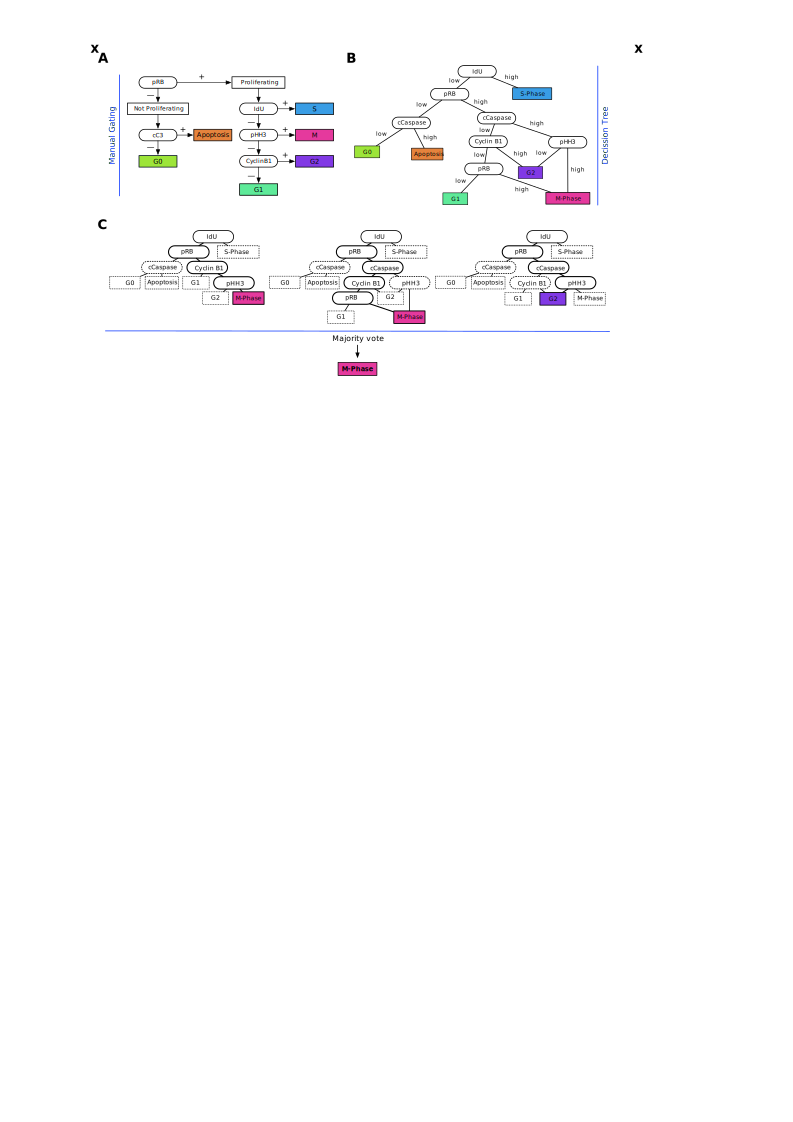
\includegraphics{03cytof/figs/3CLASS_stateRF.png}
    \caption{FINISH THIS FIGURE AND CHANGE COLORS TO MATCH METHODS}
    \label{fig:3classover}
\end{figure}

Determining a cell's state with regards to the cell-cycle phases is central to understanding the intestinal epithelium response to perturbations, as shown by Qin et \emph{al.} and their observations regarding cell-type specific regulation of cell states in response to microenvironmental and oncogenic cues~\cite{qin_cell-type-specific_2020}.

The cell states labels are commonly established using manual gating on a biaxial marker state, wherein a researches draws a boundary separating 2 groups of cells, essentially thresholding the data based on antibody expression. While strategies differ widely, a common approach taken by my lab is depicted in Figure \ref{fig:3classover}A. However, generating these cell state labels is a time consuming process, especially when compounded with the scalability of \acrshort{mc} and TOB\emph{is} ability to perform highly multiplexed analyses. Issues with user-induced biases are also present, as drawing the manual gates is a subjective process that might not remain consistent from experiment to experiment.

Early on my PhD I was exploring the link between \acrshort{ptm}s and cell state when I noticed that the process of generating the cell state labels could potentially be automated using a classical supervised machine learning approach. Eventually thus, I developed a cell state \acrlong{rf} (\acrshort{rf}) classifier to automate this process (see Chapter \ref{02methods} for more details). The manual gating process naturally resembles the logic behind a decision tree, for in both a threshold of antibody intensity would result in a binary classification of cell groups (Figure \ref{fig:3classover}A-B). Furthermore, the \acrshort{rf} machine learning approach remains a white box whose internal decision logic can be easily interpreted, for it consists of a collection of individual decision trees trained on subsets of the data that are used together in an ensemble approach (Figure \ref{fig:3classover}).

\subsection{5-marker model performs across model systems}

\begin{figure}
    \centering
    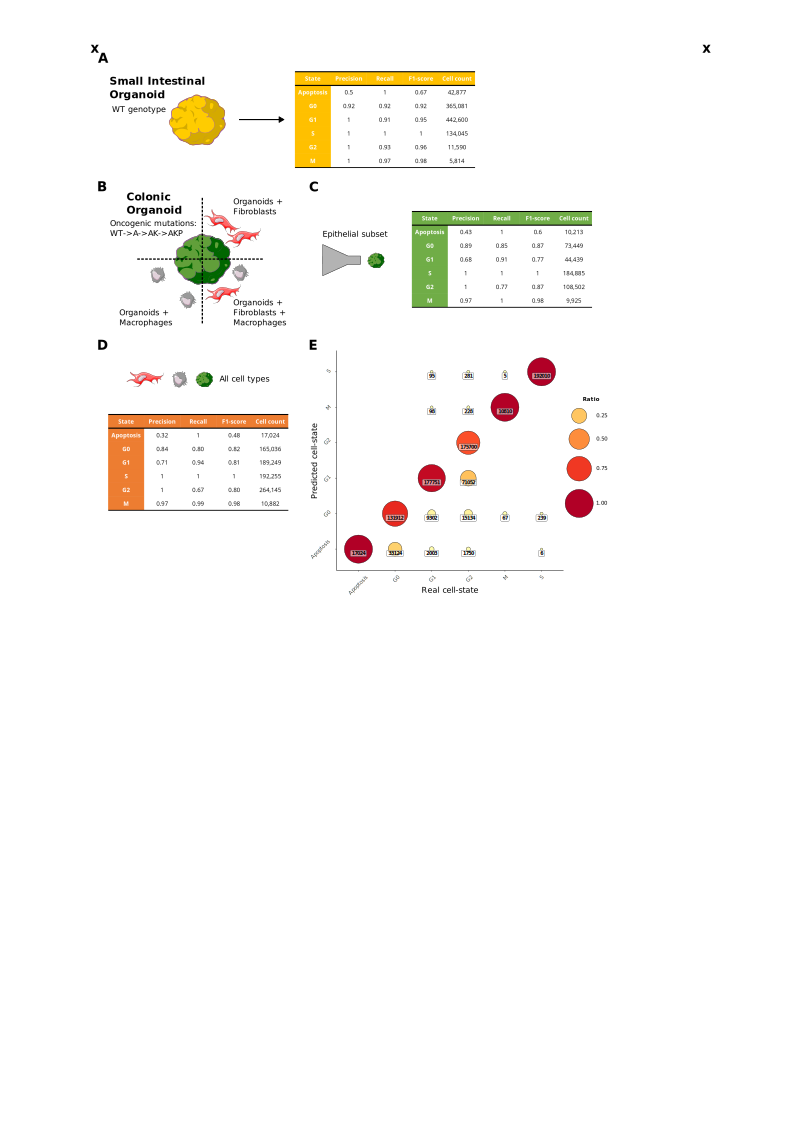
\includegraphics{03cytof/figs/3CLASS_5m.png}
    \caption{Benchmarking 5-marker RF cell state classifier. Shown in a), b), and c) are the classification reports obtained from running the 5-marker RF classifier against data manually labelled for cell state (representing the “real state” or ground truth). In a) a single timepoint SI LGR5 dataset was used, very similar to the training data for the model. The dataset in both b) and c) is a coculture of CRC organoids and their TME, with the cells in b) being a subset of the whole dataset containing just epithelial cells. Decreasing levels of performance correlate with increasing differences between the train and test datasets, as can be seen by the low f1-scores for the apoptotic class in c). Using the same data as c), the dot plot derived from the classification matrix in d) depicts the number and proportion (as both size and colour of the circles) of mislabelled cells for each cell state, showing that a considerable number of falsely mislabelled apoptotic cells are actually in G0 phase and some cells. RF: Random Forest.}
    \label{fig:3class5m}
\end{figure}

The first \acrshort{rf} model built was trained on data from the murine small intestinal organoid cultures from Qin et \emph{al.}~\cite{qin_cell-type-specific_2020}, consisting of \acrshort{wt} organoids along several developmental time points (Figure \ref{fig:3class5m}A). This model used only the 5 markers shown in Figure \ref{fig:3classover}A. Details on building the model and the relative feature importance when training can be found in Chapter \ref{02methods}.

Testing the 5-marker RF model on a different single time-point small intestinal organoid dataset also from Qin \textit{et al}. \cite{qin_cell-type-specific_2020} results in global accuracy for all classes of 0.93. However, $F_1$ scores reveal a big performance drop with the apoptotic class (Figure \ref{fig:3class5m}), driven by the low 0.5 precision score when predicting the apoptotic label. Precision scores otherwise remain above 0.92 for the other labels.

Performance of the classifier drops when testing against the CRC TME colonic organoid cultures from Qin \textit{et al}. \cite{qin_cell-type-specific_2020}. In this case, subsetting just the organoid cells from the organoid cultures (Figure \ref{fig:3class5m}B), we observe a global accuracy of 0.91. Looking at the classification details (Figure \ref{fig:3class5m}C) we see a very similar pattern to the SI LGR5 results; with the apoptotic class presenting the lowest $F_1$-scores (0.6) characterised by a low precision (0.43). Furthermore, the remaining $F_1$-scores are also lower overall, with only the S-phase and M-phase classes reaching above 0.9.

When no epithelial filter is applied to the dataset and the model performance is tested against all cell types (i.e., including also fibroblasts and macrophages) global accuracy drops down to 0.87. The relatively high global accuracy does not reflect the failure of the classifier to, yet again, identify the apoptotic cells (Figure \ref{fig:3class5m}D). In Figure \ref{fig:3class5m}E the classification matrix is used to build a dot plot in which the true labels (“Real state” from gating) are compared against the predicted labels (“Predicted state”), highlighting how a majority of the cells labelled as apoptotic are actually G0 cells, explaining the precision of 0.32 for the former class. There is also some confusion around the G2 cells, as a significant number of these cells are classified as either G0 or G1.

\subsection{10-marker model improves apoptotic classification}

\begin{figure}
    \centering
    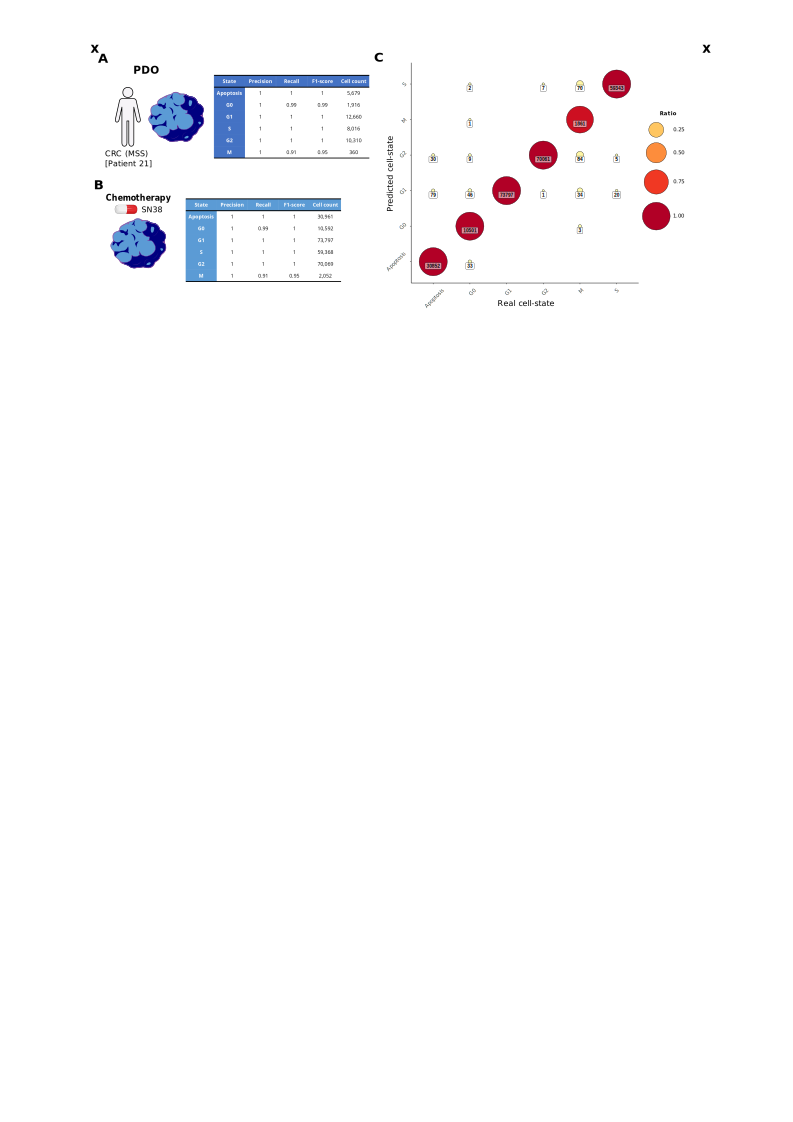
\includegraphics{03cytof/figs/3CLASS_10m.png}
    \caption{Benchmarking the new 10-marker RF cell state classifier. Building a RF classifier with an increased number of markers using data from PDOs renders better results than the original 5-marker model, as can be seen in a) with the classification report. b) Classification matrix generated automatically during model building, showing extremely low levels of misclassified cells. RF: Random Forest. PDO: Patient-Derived Organoids. Labels: 0=Apoptosis, 1=G0, 2=G1, 3=S-phase, 4=G2, 5=M-phase.}
    \label{fig:3class10m}
\end{figure}

Given the 5-marker model limitations when resolving the apoptotic class, I implemented a second model using additional \acrshort{ptm} antibodies and cell state markers targeting apoptotic cells. This 10-marker model uses a dataset from Zapatero \& Tong \emph{et al.}~\cite{zapatero_trellis_2023} wherein heterotypic \acrlong{pdo} (\acrshort{pdo}) cultures from different donors were treated with a spectrum of chemotherapies. This data was generously provided by Dr. Maria Ramos Zapatero.

Results from the updated 10-marker implementation using \acrshort{pdo} data show improved performance when compared to the 5-marker model. Using a technical replicates of the training data as test we observe how the apoptotic class gets accurately resolved (Figure \ref{fig:3class10m}A). When benchmarking the model performance against a dataset wherein the organoid cells had been treated with SN-38, the active metabolite of the type I topoisomerase inhibitor Irinotecan \cite{mathijssen_clinical_2001}, we observe a global accuracy greater than 0.99. The lowest $F_1$-scores, at 0.95, were found for the M-phase label (Figure \ref{fig:3class10m}B). This lowered, yet still accurate, prediction performance is driven by the lower total count of M-phase cells (one order of magnitude smaller than the other classes), hampering the training for that class and resulting in small number of non-apoptotic cells to be miss-labeled as M-phase.
In contrast with the 5-marker model results, there is an apparent lack of issues when classifying the apoptotic class, with only 0.35\% of true apoptotic cells being mislabelled (Figure \ref{fig:3class10m}).

\newpage
\section{Conclusions}

In this chapter I have shown how CyGNAL is an accessible workflow to non-computational users that facilitates data processing and analysis of \acrshort{mc} experiments. The computation of \acrshort{emd} and \acrshort{dremi} scores enables a detailed mechanistic description of changes across conditions, wherein changes in the user defined reference allows for differential interrogation of the experimental system. 

While the scores themselves can be used to build curated mechanistic models as in Qin \emph{et al.} \cite{qin_cell-type-specific_2020}, CyGNAL also incorporates interactive visualisation modules that can automatically plot results. The interactive nature of the visualisation steps, coupled with additional data correlation metrics given during the \acrshort{pca} computation, allows for both exploratory data analysis and (close to) publication grade results generation within a single tool. This same \acrshort{pca} computation presents a straightforward way to summarise changes at the condition level from otherwise information-dense \acrshort{emd} or \acrshort{dremi} heatmaps.

The incorporation of miscellaneous data handling helper scripts in the utilities folder exemplifies how user-provided feedback is paramount, while it also signifies how CyGNAL continuously grows and changes with time. Tools are meant to be used, and that publications by colleagues such as Michelozzi \emph{et al.}~\cite{michelozzi_activation_2023} employed CyGNAL is a testament to its accessibility.

Originally meant as a simple exercise in curiosity-driven exploration after noticing the correlation between so called PTM and "cell state" markers, and empowered by the tediousness of manually gating the datasets in our lab, the \acrshort{rf} cell-state classifier has become a convenient tool to automate cell-state labelling of \acrshort{mc} datasets in relation to cell-cycle phases.

Albeit a very simple model, the nature of the manual gating process (essentially thresholding on a biaxial space of marker expression) translates well to decision trees, and this is shown in the relatively strong overall model performance. The current implementation however, might struggle to generalise to external datasets, for gating strategies are somewhat of a lab- and individual-specific process.

Where we do observe weak points in the classifier is for those cell state labels whose antibody coverage is not great in the model. For example, in the 5-marker \acrshort{rf} model, apoptotic cell class precision reaches only 0.32 in the most stringent setting tested (Figure \ref{fig:3class5m}D). This can be relatively straightforward to address by increasing the number of antibodies targeting that particular state (Figure \ref{fig:3class10m}B-C), but this strategy can not always be employed as the additional marker would both need to be in the reference data used to train the model and in the query dataset to be labelled. When possible however, as demonstrated by the the 10-marker \acrshort{rf} model built, high precision and recall scores are accomplished for all cell states even in the context of cell-cycle disrupting chemotherapy (Figure \ref{fig:3class10m}B-C).

As described in Chapter \ref{02methods}, both tools are publicly accessible in their respective GitHub repositories. 
\chapter{Stromal and Oncogenic Regulation of Colonic Stem Cell Polarisation}
\label{04seq}

\section{Introduction}


AIMS
% Both the SI LGR5 and the colonic organoid systems have been thoroughly characterised before at the mass cytometry level and, to better understand these systems, we aim to perform a comparative characterisation of the organoids using scRNA-seq. 
% Given the well-known biology of the murine small intestine at the transcriptome level21, we can analyse the SI LGR5s to characterise the different subpopulations within the epithelial organoids and cross-validate the results with in vivo scRNA-seq studies and the mass cytometry results discussed above11. In a similar fashion, we also aim to characterise the colonic organoids and the stromal and immune compartments that form the TME in the heterocellular cultures. Unlike mass cytometry, which requires tailored panels of antibodies reaching only into a few dozens, with scRNA-seq we will be able to characterise thousands of genes at once in the organoids, fibroblasts, and macrophages. 
% Leveraging the publicly available ligand-receptor databases mentioned in the background section, data from the scRNA-seq experiments will be used to identify the ligands and receptors expressed in the colonic heterocellular organoid cocultures. 
% The cell communication information gathered this way can then be summarised as signalling pathways that define and connect the different populations of cells. Furthermore, the study of this interactome would aid towards understanding the interplay between the CRC organoid model and its TME. This can be achieved by comparing the cell communication results with the intracellular PTM signalling described in Qin et al. 2020 and seeing how cellular communications change in cultures mimicking an oncogenic setting.

\subsubsection{Figure on experimental design, with the 2 axes of perturbation}

\section{Organoids recapitulate colonic epithelial cell states}

\subsubsection{Figure on Integrated object DR, and expression of cannonical markers in control condition}

\section{Oncogenic mutations and fibroblasts polarise epithelia towards distinct stem cell fates}

\subsubsection{Figure on DA overview and individual DA tests}

\subsubsection{Figure on signalling entropy, RNA velocity changes, and CellRank sinks}

\section{Oncogenic mutations block fibroblast to epithelia signalling}

\subsubsection{Figure on cell-cell communication analysis}

\section{Characterisation and relevance of proCSC and revCSC}

\subsubsection{Figure on stem signatures and key signalling pathways}

\section{Conclusions}






\chapter{Data-driven Landscapes of Colon Epithelial Plasticity}
\label{05vr}

\section{Introduction}

\section{Valley-Ridge scores as a landscape of colonic epithelial cell-fate plasticity}

\subsubsection{Figure on VR score definition}

Correlation of VR score with CCAT and with Origins for each cell, grouped by clusters

\subsubsection{Figure on VR Waddington-like landscapes}



\section{Conclusions}






\chapter{Knowledge Graphs for Cell Communications}
\label{06kg}

\section{Introduction}

\begin{figure}
    \centering
    \includegraphics{06kg/figs/6KG_com.png}
    \caption{}
    \label{fig:6intro}
\end{figure}

Cellular signalling involves a complex series of directed and hierarchical~\cite{kumar_3_2003} signal transduction cascades between molecules that dictate a cell's response to extrinsic and intrinsic cues.

In the context of inter-cellular paracrine communication for example, a secreting cell produces a series of ligands that are captured by receptors on a receiving cell. The receiving cell then might engage in an intra-cellular signal transduction cascade orchestrated by \acrshort{ptm}s, such as the MAPK cascade~\cite{zhang_mapk_2002}. These cascades regulate gene expression downstream of active transcription factors. With overlapping pathways, feedback loops, and complex settings with multiple cells engaging in symmetrical or non-symmetrical communications, there is nonetheless a directional causality-driven signalling information flow (Figure \ref{fig:6intro}).

The physical interactions between molecules are often represented as a network of genes, proteins or even \acrshort{ptm}s, described in the manner of a \acrfull{kg}. These network representations have been extensively explored to model both intra- and inter-cellular communications, but to date they are not consistently analysed using methods that leverage the underlying directed and hierarchical nature of signalling processes, often either treating the graph as undirected or analyzing pairwise relationships between feature detection metrics (such as gene expression)~\cite{pratapa_benchmarking_2020, armingol_deciphering_2020}. 
    % Cellular signaling involves overlapping directed \cite{HANCOCK200364} and hierarchical signal transduction cascades between molecules to coordinate targeted behavior \cite{zhang_mapk_2002}.
    % %The physical interactions of molecules are often represented as a network.
    % The resulting network of molecular interactions determines a cell's response under different conditions, drawing interest towards unifying and characterizing varying sources of molecule signaling from distinct scientific experiments. However, methods to represent biological networks and infer gene-gene relationships rarely take into the account the \textit{directionality} and \textit{hierarchical structure} of these gene graphs.

The field of directed cellular interaction databases already presents with some established curated resources like OmniPath~\cite{turei_integrated_2021}, with a growing number of methods attempting to model the communications in a directed manner~\cite{lefebvre_large-scale_2021}, describing cell-cell interactions~\cite{fischer_modeling_2022,yang_sctenifoldxct_2023}, and even data-driven \emph{de novo} generation of signal transduction networks~\cite{hu_cytotalk_2021}.

Knowledge graph embedding tools aim to learn the complex relational information in heterogeneous directed networks and represent it in a lower dimensional space that can be analysed using more common graph signalling processing and general data analysis approaches. Methods like the classical TransE~\cite{bordes_translating_2013} and its derivatives, graph convolutional networks, and hyperbolic embeddings~\cite{chami_hyperbolic_2019}, represent some of different approaches to learn the strcuture of \acrshort{kg}s.

In this chapter I propose a novel approach for assembling gene-gene graphs that capture cellular communications by leveraging \acrshort{kg} embedding approaches. I aim to project single-cell \emph{omic} profiles into the assembled \acrshort{kg}s, thus treating the cells as signals on a gene graph. The resulting signals can then be treated as another single-cell \emph{omic} view of the cells, and used to generate new embeddings or be compared against their gene expression profiles.

        % Gene embedding methods are growing , so are graph signal processing approaches. 
        % Discuss the embedding methods of these graphs:
        % Complexity in terms of structure, directionality and type of interaction. All of this is very important, unlike in undirected knn grpahs ubiquitous to omic analyses.
        % This means that we need some methods able to compute all of this complex relations in multi relation directed graphs  (MultiDiGraph). methods have been developed, transE \cite{bordes_translating_2013}family, graph convolutional networks, and the stuff from he stanford dawn group on  hyperbolic embeddings  \cite{chami_hyperbolic_2019} and general ML approaches applied to non euclidean spaces.
        % Non-euclidean space like hyperbolic spaces argued to be key because graphs with important hierarchical structure [as is biological signalling] is much better capture in a hyperbole than in a plane \cite{bronstein_geometric_2017,nickel_poincare_2017,chamberlain_neural_2017}.[the first one is general Euclidean =bad, the later ones refer to the cocnept of hierarchical graph better on hyperboles than planes].
        % on the other hand, prelim results in collab porject suggest perhaps not as important for bio KG despite the hierarchical nature of signalling networks.



\section{KG Structure}

\begin{figure}
    \centering
    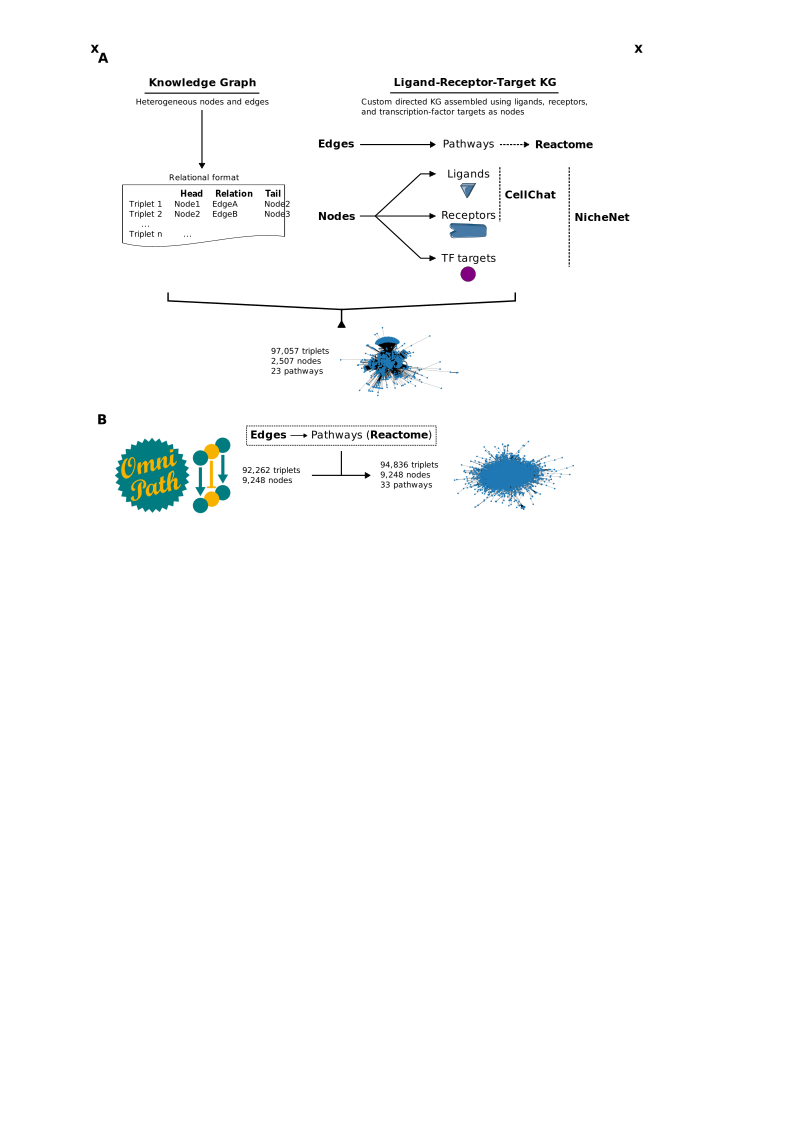
\includegraphics{06kg/figs/6KG_kg.png}
    \caption{}
    \label{fig:6kg}
\end{figure}

Graph assembled from sources, hierarchical directed structure. Nodes are ligands, receptor and gene targets of cellular signalling. Edges established from pathway connecting two nodes. Sources are cellchat and nichenet for nodes and reactome for pathways.

Formatted as head,relation,tail format. Total of XX relations with YY and ZZ nodes.

Compare against common KG such as OmniPath.
Omnipath has a curated functional interactions interaction database comprising genes involved in cellular communications. type of interactions (PTM, ...) consensus, directionality and even logical sense of interaction (activation or repression). HTis datasbase is cureated from public resources.
Process interaction database as before by using OmniPath nodes and edges from reactome pathways. 
Comparable graph in terms of node, but a bit more dense than the LRT KG and with a lower hierarchy score (see Chapter \ref{02methods} for Table \ref{tab:2kg}).



\section{KG Embedding}

\begin{figure}
    \centering
    \includegraphics{06kg/figs/6KG_embed.png}
    \caption{}
    \label{fig:6embed}
\end{figure}

To capture the complex relational information in a simpler format amenable to downstream analyses, .....

Leverage directed nature of graph by embedding on lower space. Methods used (Chapter \ref{02methods}). Exploration of nodes on a DimRed space suggest I can capture topological differences between Ligands , receptors and targets. It also appears that gene targets are the most promiscuous nodes with higher degrees, followed by receptors and finally ligands. However, care must be taken here for three classes are imbalanced.

Biological information is also capture in the KGE, with nodes showing a certain degree of separation by key signalling pathways from REACTOME.
    Looking at nodes thsi means thatwe can see which kind of genes (lignas, receptors, targets,...) are present and how they dsitribute. 


% Finally, embedding representation of relations (edges) can be generated, which should capture relations between pathways. Recover high level groupins of pathways with similar biological function, due to their shared nodes on KG.
%     WE can also check out the different pathawys they belong to and see if there is come kind of biologically driver distribution here re pathways. Edges can also be embedded and hopefully lowere level pthawys belonging to a shared bigger levl pathways might lie in closer together? Also deppening on the ratio of shared interactions members between disticnt pathways. 

\section{Cells as Signals on a Gene Graph}

\begin{figure}
    \centering
    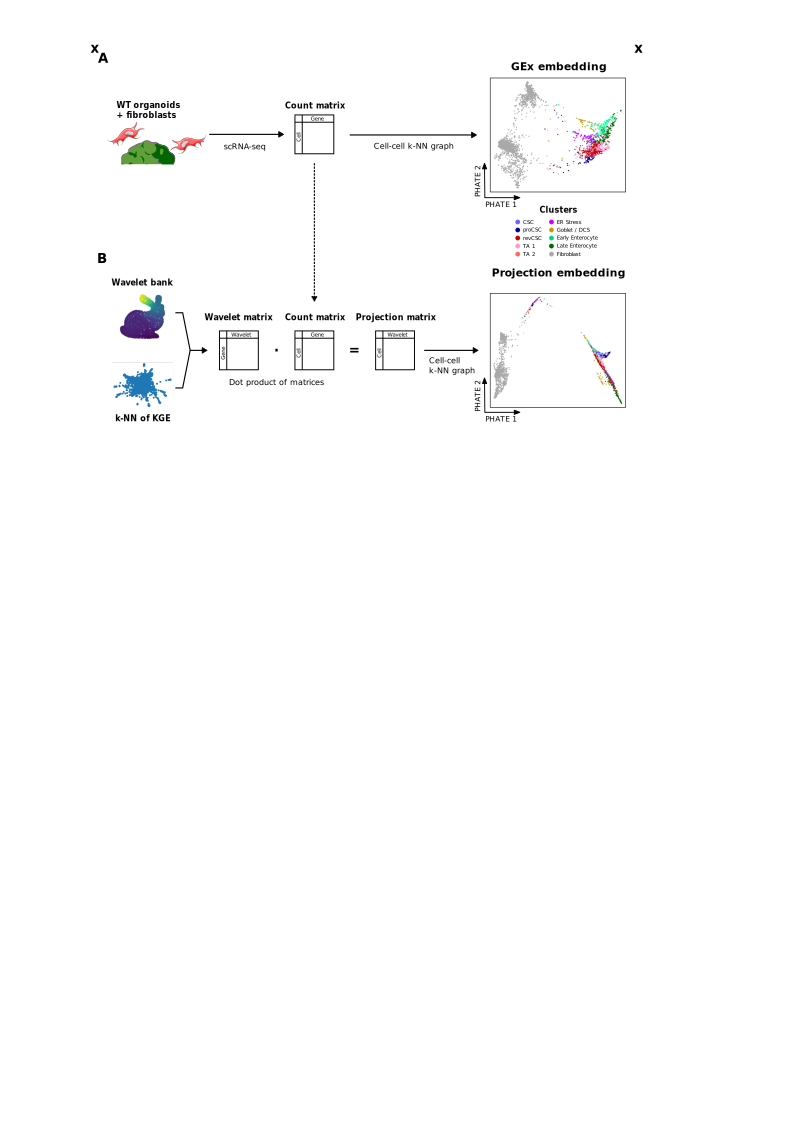
\includegraphics{06kg/figs/6KG_projection.png}
    \caption{}
    \label{fig:6project}
\end{figure}

Organoid dataset. Wt stromal coculture where fibs talk to WT epi cells (Figure \ref{fig:4cc}A). Embed count matrix reveals 2 cells types and epithelial heterogeneity.

Given the KGE, generate a \emph{k}-NN graph onto which I apply a wavelet bank on nodes at series of scales. This difussion process generates a wavelet matrix onto which the gene expression matrix can be projected.

Leveraging the properties of the dot product (\(\cdot\)) operation between matrices, I compute the product between the \(node X wavelets\) matrix and the \(cell X feature\) count matrix, where the features are formatted as gene symbols like in the \acrshort{kg}. This results in a new projected matrix of \(cell X wavelets\) dimensions (Figure \ref{}).

Resulting projection topologically resembles GEx data on PHATE embedding, albeit it appears there is some signal loss as epithelial heterogeneity is not as noticeable.

\begin{figure}
    \centering
    \includegraphics{06kg/figs/6KG_bench.png}
    \caption{}
    \label{fig:6bench}
\end{figure}

Porjection results can be assed quantitaively by comparing cell-cell distance between the GEx graph and projected graph. given what we know on fibs interacting with revCSC and TA 2, wee would expectd thos differences to be decreased on projected space.

We thus construcut 2 knn, from gex and from LRT projection, and then compute the median/average distance between clusters. To compare two distance datasets, relative values established.

Mixed results tbh.

\newpage
\section{Conclusions}

\colorbox{yellow}{OUTLINE (WIP)}
* Built LRT KG that is comparable to other directed graphs in literature.
    * IF omnpath capture ground bio truth, cell commns are indeed mostly hierarhcical. WE have a simplified hyper hierarhcical version.
* KG embedding methods seem to conserve biological properties associted with nodes.
* Wavelets used to difusse signal on graph so that single-cell \emph{omic} data can be projected on it.
* Results match/conserve broader GEx information, but information gain is limited regarding cell communications.
* Need to improve signal difussion step. Alternative gene embedding step can also be explored (GSP paper), so can the benchmarking be improved.

Fine balance between signal loss determined by lmited number of gene nodes on graph, but also on graph structure itself being important enough to produce results signficantly different from GEx matrix.
\chapter{Discussion and Future Perspectives}
\label{07disc}

\section{Building Accessible and Automated Tools for MC Data Analysis}

In this work I have shown CyGNAL's capabilities, describing in detail its design and inner mechanisms, and outlining its usefulness with regards to the analysis of \acrshort{mc} datasets.

The main testament for the usefulness of the tool is the fact that it has become a part of routine \acrshort{mc} analyses in our lab. With its support for plain text to FCS inter-compatibility (Chapter \ref{02methods} and Figure \ref{fig:3cygpipe}), users can seamlessly integrate with \acrshort{mc} platforms such as Cytobank. Given that the user only needs to run simple Python commands on the terminal to use CyGNAL, it has been readily adopted in day-to-day lab use even by users with no advanced computing experience. 
As I have shown in Chapters \ref{02methods} and \ref{03cytof}, CyGNAL is able to perform a comprehensive analysis of changes occurring across multiple conditions of the often wide \acrshort{mc} experimental systems. Designed for the study of \acrshort{ptm} signalling changes, CyGNAL's computation of \acrshort{emd} and \acrshort{dremi} scores resolves marker intensity and connectivity changes (Figure \ref{fig:3cyguse}). The intuitive and customisable interactive Shiny-Apps allow for exploratory and close to publication-grade visualisation of the results (Figure \ref{fig:3cygvis}). Tools are meant to be used, and that publications by colleagues such as Michelozzi \emph{et al}.~\cite{michelozzi_activation_2023} employed CyGNAL is a testament to its relevance.

Originally meant as a simple exercise in curiosity-driven exploration after noticing the correlation between so called PTM and 'cell-state' markers, and empowered by the tediousness of manually gating the datasets in our lab, the \acrshort{rf} cell-state classifier has become a convenient tool to automate cell-state labelling of \acrshort{mc} datasets in relation to cell-cycle phases.

Built around a simple \acrfull{rf} architecture, the \acrshort{rf} classifier benefits from the fundamental gate-like logic of both decision trees and the manual cell-state gating process (Figure \ref{fig:3classover}). However, I expect the classifier to suffer from generalisation issues when dealing with external data labelled using different workflows. Furthermore, even if it leverages fuzzy logic to match channel names from the model to the input data, the classifier still relies on matching markers found in both the training  and test datasets. While the markers dedicated to apoptosis and cell-cycle phases generally belong to the less variable portions of \acrshort{mc} panel design (Table \ref{tab:2rfmark}), this can still pose an inconvenience when deploying the model. However, I have also shown how weak points such as low performance for apoptotic class prediction using the 5-marker \acrshort{mc} model (Figure \ref{fig:3class5m}), can be effectively addressed by just the addition of an additional apoptotic marker to the panel design (Figure \ref{fig:3class5m}A). Furthermore, the model seems resilient to cell-type composition and even to broad cell-state changes induced by chemotherapy (Figure \ref{fig:3class5m}B-C).

Hearkening back to the link between \acrshort{ptm}s and cell-cycle, the 10-marker \acrshort{mc} model also reveals how certain \acrshort{ptm}s prove more informative when training than \emph{bona fide} 'cell-state' markers (Figure \ref{fig:2train}E). Furthermore, discrepancies between expected cell-state and \acrshort{ptm} correlations from the literature and feature importance rankings have anecdotally been used to validate under-performing antibodies with high unspecific background staining.

Both these tools remain under continuous support, and I aim to eventually merge both code bases and integrate automated cell-state classification into CyGNAL using pre-built classifier models or allowing for the generation of new models based on specific user-provided labelled data.
CyGNAL could also be augmented by the addition of PHATE~\cite{moon_visualizing_2019} as an alternative \acrshort{dr} step, implementing a new Shiny-App to visualise the embeddings and overlay user-selected metadata or antibody intensities.

\newpage
\section{Charting Stromal and Oncogenic Regulation of CSC Polarisation}

Single-cell technologies can describe cell-cell communications and cell-type transitions in complex organoid settings and \emph{in vivo} tissues~\cite{qin_deciphering_2020, jin_inference_2021, bues_deterministic_2022}. As shown in Qin \emph{et al.}~\cite{qin_cell-type-specific_2020}, a heterocellular colonic epithelia organoid system can be employed in experimental designs covering the effects of both intrinsic \acrshort{crc} oncogenic mutations and extrinsic environmental cues. However, the directed and limited nature of the \acrshort{mc} antibody panels used in Qin \emph{et al.}~\cite{qin_cell-type-specific_2020} presented with a limiting factor towards a detailed description of colonic organoid epithelial polarisation by intrinsic and extrinsic cues. 

Therefore, in Chapters \ref{04seq} and \ref{05vr} I have employed a multiplexed \acrshort{scrnaseq} analysis of heterocellular \acrshort{crc} organoid cultures (Figure \ref{fig:4exp}) to chart a continuous landscape of intrinsic and extrinsic regulation of \acrshort{csc} states. I have found that stromal cues transition the epithelia towards the \acrshort{revcsc} state, oncogenic signalling pushes the organoid towards \acrshort{procsc}, and exogenous ligands overlapping with both stromal and oncogenic signalling cues can polarise towards both states at once (Figure \ref{fig:4da}). I have also developed a method to capture these transitional processes, the \acrfull{vr} score (Figure \ref{fig:5score}), and established a workflow to project it onto Waddington-like data-driven landscapes (Figure \ref{fig:2land}). 
The work presented in this thesis was paired with complementary \acrshort{mc} experiments in Qin \& Cardoso Rodriguez \emph{et al.}~\cite{cardoso_rodriguez_single-cell_2023}, where we interrogated colonic stem cell regulation at scale to functionally understand the polarisation mechanisms (Appendix \ref{appendix:qincardoso}).

First, I have shown that transcriptomic profiles of epithelial, fibroblast and macrophage cells from the heterocellular cultures can be used to describe inter-type heterogeneity and recapitulate the distinct epithelial compartments (Figures \ref{fig:4exp} \& \ref{fig:4intepi}). 
The observed \emph{Cd34} high and low fibroblast populations are reminiscent of \emph{in situ} intestinal fibroblast heterogeneity, wherein \emph{Cd34} expressing fibroblast from the bottom of the crypts support the intestinal stem niche~\cite{stzepourginski_cd34_2017} whereas \emph{Cd34} low fibroblast are found above the crypt's bottoms and help maintain the BMP gradient needed for epithelial differentiation~\cite{karpus_colonic_2019}. While I observed some transcriptional differences between these two fibroblast populations (Sup. Figure \ref{fig:defib}), their regulation of the epithelial compartment remained consistent (Sup. Figure \ref{fig:deepibyfib}), possibly due to shared secreted signalling between the two. 
Myeloid macrophage transcriptomes formed a continuum trajectory of putative inflammation-related roles (Sup. Figure \ref{fig:demac}), unlike the distinct fibroblast and epithelial populations. However, neither macrophages as a whole nor the extremes of their transcriptional continuum differentially regulated the epithelial cells.

The healthy small intestinal and colonic epithelia is supported by a stem cell niche at the bottom of the crypts regulated by both intrinsic and stroma-secreted signalling gradients. These traditional \acrfull{csc} however, are not the sole stem cell state, with less common low-proliferative \acrfull{revcsc} being able to replenish the \acrshort{csc} niche and repair the epithelial tissue in response to tissue damage~\cite{ayyaz_single-cell_2019}. Here I have shown how these \acrshort{revcsc} are enriched by stromal WNT and TGF-\textbeta\hspace{0.1cm} when \acrshort{wt} organoids are co-cultured with fibroblasts (Figures \ref{fig:4da}A \& \ref{fig:4cc}B), and how \acrshort{revcsc} also resemble public descriptions of the same population and a “foetal"-like state~\cite{mustata_identification_2013} (Figure \ref{fig:4sign}A).

The gradient of organoids with accumulating oncogenic mutations revealed how a \acrfull{procsc} state is enriched in CRC organoids (Figure \ref{fig:4da}B). These cells are present in lower numbers in \acrshort{wt} and \textit{shApc} organoids, but quickly dominate the landscape of stunted absorptive and secretory differentiation in the \textit{shApc} and \textit{Kras\textsuperscript{G12D/+}} (AK), and \textit{shApc}, \textit{Kras\textsuperscript{G12D/+}} and \textit{Trp53\textsuperscript{R172H/–}} (AKP) colonic organoids (Figure \ref{fig:4da}C). \acrshort{procsc} were found to be transcriptionally similar to other cells from mouse models and human CRC (Figure \ref{fig:4sign}A).

With a clear differential regulation by extrinsic stromal cues and intrinsic oncogenic signalling, polarisation of \acrshort{wt} colonic epithelia towards both \acrshort{procsc} and \acrshort{revcsc} could nonetheless be achieved via exogenous WENR added to the culture media (Figure \ref{fig:4da}C). These findings, together with subsequent \acrshort{mc} validation~\cite{cardoso_rodriguez_single-cell_2023} of the signalling hubs identified via cell-cell communication analysis, suggest that both states are part of a shared polarisation landscape with overlapping signalling pathways that compete to establish colonic epithelial cell-fate.
In this context, the observed breakdown of fibroblast-to epithelia communications in CRC organoids (at least partly due to downregulation of key signalling receptors by the epithelial cells) seems to suggest that intrinsic oncogenic cues dominate extrinsic stromal cues (Figure \ref{fig:4cc}). The interplay between the two with regard to \acrshort{procsc} and \acrshort{revcsc} polarisation is explored further in Qin \& Cardoso Rodriguez \emph{et al.}~\cite{cardoso_rodriguez_single-cell_2023}, where we established that TGF-\textbeta\hspace{0.1cm} can induce \acrshort{revcsc}-like cells in CRC organoids in the context of low PI3K signalling, supporting the suggested role of \acrshort{revcsc} as a drug-resistant state in CRC that can drive relapse after chemotherapy~\cite{alvarez-varela_mex3a_2022, zapatero_trellis_2023}.

\emph{In silico} analysis of cellular dynamics identifies \acrshort{revcsc} as a terminal cell-fate (Figure \ref{fig:4dyn}E), suggesting that polarisation of the colonic epithelia towards \acrshort{revcsc} is achieved via plasticity-driven transitional processes from adjacent cell-states. In contrast, \acrshort{procsc} is consistently identified as an initial population (Figure \ref{fig:4dyn}) whose dominance of the epithelia seems to be achieved due to its high proliferative potential.

Therefore, I postulated that cellular pluripotency scores and rates of transcriptomic change could capture the cellular dynamics of such systems, providing for an avenue towards generation of data-driven Waddington-like landscapes of cellular differentiation and plasticity. The \acrfull{vr} score described in Chapter \ref{05vr} synthesises both CCAT and RNA velocity vector length metrics to capture coarse pluripotency changes and global transcriptomic structure with PHATE. Finer details at a local level capture the availability of cell-states as determined by RNA velocity (Figure \ref{fig:5score}). The methodology presented also incorporates with a landscape projection pipeline (Figure \ref{fig:2land}). The \acrshort{vr} landscapes reconstruct the shared landscape of colonic stem cell polarisation, presenting \acrshort{revcsc} as an accessible epithelial fate in the presence of stromal ligands, whereas intrinsic oncogenic signalling trap the organoid in a highly pluripotent yet isolated \acrshort{procsc} fate, refractory to stromal signals that otherwise would polarise the cells towards \acrshort{revcsc} (Figure \ref{fig:5land}). 

The work presented in these two chapters presents with some notable limitations, such as a lack of non-organoid \emph{in situ} validation: with the only effort towards validating the findings being achieved via \emph{in silico} signature matching and data integration (Figure \ref{fig:4sign}). Furthermore, non-paracrine stromal regulation, specially given the well-known role of fibroblasts as extra-cellular matrix re-modellers, has not been deeply explored in this study. It is also worth noting that a line of normal murine intestinal fibroblasts was used in the organoid co-cultures, rather than pairing the \acrshort{crc} organoids with cancer-associated fibroblasts. 
This later point will be addressed in subsequent studies at the lab by attempting to match patient-derived organoids with cancer-associated fibroblasts from the same donor. Further work regarding the cross-validation with human data of the \acrshort{procsc} and \acrshort{revcsc} cell identities and functional characteristics is being carried out as part of the peer-review process of the work presented in Qin \& Cardoso Rodriguez \emph{et al.}~\cite{cardoso_rodriguez_single-cell_2023}. Furthermore, additional improvements to the \acrshort{vr} score and landscape generation will be implemented during the later stages of my project. Aiming to increase the tool's accessibility and ease of use, the current Jupyter Notebook format will be adapted to the nbdev framework (\url{https://nbdev.fast.ai/}). \acrshort{vr} landscapes will be packaged as a tool, \emph{\acrshort{vr} Land} (\url{github.com/FerranC96/VRland}), which will be distributed as an interactive web-app to facilitate the exploration of the 3-dimensional landscapes generated.

In conclusion, these results describe fibroblasts as key stromal regulators of the colonic stem compartment, orientating epithelial stem cell fate via secreted WNT and TGF-\textbeta\hspace{0.1cm}. Stromal regulation competes with, and is ultimately trumped by, the \acrshort{procsc}-enriching organoid-intrinsic oncogenic cues. Further understanding concerning the regulation of \acrshort{procsc} and \acrshort{revcsc} fates might suggest new avenues for cancer therapies. Indeed, given that \acrshort{revcsc} has already been described as a drug-tolerant persister state~\cite{alvarez-varela_mex3a_2022}, blocking the plastic processes controlling its accessibility might be a valid strategy to limit the emergence of chemotherapy resistance. 


\newpage
\section{Knowledge Graphs for Cell Communication}

While cellular communications are commonly understood to be a complex process both at the inter- and intra-cellular levels, there is a lack of tools aiming to capture the causal and directed nature of the process. Coupled with emerging multi-modal approaches that could measure gene and protein expression, including \acrshort{ptm}s, methods capturing both paracrine secreted signalling and cell-state responses to extrinsic cues should describe a holistic view of cellular communications.

In Chapter \ref{06kg} I have assembled a directed and hierarchical \acrfull{lrtkg} from publicly available databases that aims to capture the cellular signalling occurring both between interacting cells and within a cell receiving extrinsic cues (Figure \ref{fig:6intro}). Aiming to apply this new method to study cell communications within the \acrshort{wt} organoid and fibroblast co-culture in a holistic manner, the assembled \acrshort{kg} has a complexity comparable to the curated OmniPath database (Figure \ref{fig:6kg}, Table \ref{tab:2kg}). Nonetheless, I have shown that knowledge graph embedding approaches can learn a simpler tabular representation of the \acrshort{kg} that conserves the biological information encoded within it; including relational information between the gene nodes regarding pathway annotations (Figure \ref{fig:6embed}). 

Using a wavelet-based diffusion step and projecting the \acrshort{scrnaseq} organoid co-culture data (Figures \ref{fig:2wav} \& \ref{fig:6project}), I have successfully shown that projected cellular profiles diffused on the \acrshort{kg} preserve the information encoded in the original transcriptomic data representation. However, the projected profiles appear to be too similar to the \acrfull{gex} data (Figure \ref{fig:6project}). Indeed, when inter-cluster distances are computed, no significant change was detected between the original and projected views; with fibroblasts and \acrshort{revcsc}s, found to be closely interacting by cell-cell communication, remaining at comparable proximity to their prior \acrshort{gex} profiles (Figure \ref{fig:6bench}).

Most likely explained by an insufficient diffusion process, alternative approaches are being explored in conjunction with my collaborators at Yale University; such as the work on directed scattering transforms presented at the Graph Signal Processing Workshop 2023 (\url{https://ferranc96.github.io/posts/GSPw23/}). With a robust diffusion process, the method performance could also be bench-marked by leveraging spatial data as done by alternative cell-cell communication approaches~\cite{fischer_modeling_2022}. Multi-modal data could also be projected on a modality-agnostic feature-feature \acrshort{kg} with both protein and gene nodes. This approach should be able to more confidently call inter-cellular interactions via ligand-receptor expression, and intra-cellular responses via \acrshort{ptm} profiles and expression of transcription factor targets.

In summary, a balance between limiting signal loss (determined by the nodes in the \acrshort{kg}) and adequate diffusion approaches (ensuring sufficient information on the graph structure itself is captured during data projection) is necessary for such a holistic cell communication method to perform adequately. It would appear then, that the current implementation requires of further work on the later point. Published approaches exist to tackle similar problems~\cite{lefebvre_large-scale_2021, yang_sctenifoldxct_2023}, but the aim of treating the cells as signals to be compared on a gene-gene graph (or other \emph{omic} features), remains to my knowledge unique to the efforts presented here and worth pursuing specially considering multi-modal profiles could be projected on such feature-feature \acrshort{kg}s. 

\phantomsection
\addcontentsline{toc}{chapter}{Appendices}

% The \appendix command resets the chapter counter, and changes the chapter numbering scheme to capital letters.
%\chapter{Appendices}
\appendix

\chapter{pyKrack}
\label{appendix:pykrack}

CAHpter on pykrack as a package. Concept of hierachy in a graph. Krackhadt heirahrcy. 

Implementaiotn in Python

Compare against already existing R implemtnation.
using nbdev for coding, vignettes, documentation, packaging and plublishing (to pypi).

Some kind of figure here

\section{Introduction}

Biological signaling can be modeled as a directed network, where nodes represent genes/proteins and edges represent signaling interactions.

The hierarchy of such a network can be quantified using various metrics, including the Krackhardt hierarchy score. This score measures the degree to which the network exhibits a perfect hierarchy, with higher scores indicating greater hierarchy.

In R the sna package presents methods to compute graph hierarchy including Krackhardt’s score (defined as
where is the number of unordered pairs of points in Dr that are asymmetrically linked), and there are other hierarchy scores implemented in Python such as Flow Hierarchy Score Luo and Magee 2011. However, despite its utility, there is currently no native implementation of the Krackhardt hierarchy score in Python.

\subsection{Krackhardt hierarchy score}

As defined in Krackhardt, David. (1994). Graph Theoretical Dimensions of Informal Organization. Computational Organization Theory. 89.

The graph hierarchy condition states that in a digraph D, for each pair of points where one (Pi) can reach another (Pj), the second (Pj) can't reach the first (Pi). 
For example, in a formal organization chart a high lvl employee can reach through the chain of command her subordinate's subordinate. If the formal organization is working "properly", this lower lvl employee can't simultaneously reach the high lvl employee.
To measure the degree of hierarchy of digraph D, a new digraph Dr must be created. Dr is defined as the reachability digraph of D. Each point in D exists in Dr; moreover, the line (Pi,Pj) exists in Dr if and only if Pi can reach Pj in D. If D is graph hierarchic, then Dr will have no symmetric lines in it (i.e. if the line (Pi,Pj) exists in Dr then the line (Pj,Pi) does not).

The degree of hierarchy then is defined as:

Where is the number of unordered pairs of points in Dr that are symmetrically linked , and the number of unordered pairs of points in Dr where Pi is linked to Pj or viceversa.

%%%%%%%%

The Krackhardt hierarchy score is given by the following equation:

\begin{equation}
H_i = \frac{\sum_{j \in P_i} w_{ij} H_j}{k_i}
\end{equation}

where $H_i$ is the hierarchy score for node $i$, $P_i$ is the set of direct reports of node $i$, $w_{ij}$ is the weight of the edge between nodes $i$ and $j$, and $k_i$ is the number of direct reports of node $i$.

This equation calculates the hierarchy score for each node in a network based on the hierarchy scores of its direct reports and the weights of the edges between them. The hierarchy score represents the level of influence or power that a node has in the network, with higher scores indicating greater influence.


\section{Implementation}

\subsection{compute hierarchy function}

\subsection{nbdev paltform}




\chapter{Supplementary Figures}
\label{appendix:SupFig}

\section{Figures related to Chapter \ref{04seq}}

\begin{figure}[h!]
    \centering
    \includegraphics{0Xappendices/0XSup_DEfib.png}
    \caption{}
    \label{sfig:defib}
\end{figure}

\begin{figure}[h!]
    \centering
    \includegraphics{0Xappendices/0XSup_DEepibyfib.png}
    \caption{}
    \label{sfig:deepibyfib}
\end{figure}

\begin{figure}[h!]
    \centering
    \includegraphics{0Xappendices/0XSup_DEmac.png}
    \caption{}
    \label{sfig:demac}
\end{figure}

\chapter{Supplementary Tables}
\label{appendix:SupTab}

\section{Gene Data}

\newpage
\begin{table}[H]
  \centering
  \caption{\textbf{Colonic epithelia gene markers (1/2)}. MArkers of epithelia populatin and orgnaoid genotypes. Derived from literature and DE analysis of our data.}
  \label{tab:epimarkers}
  \csvreader[
    tabular=|c|c|,
    head=true,
    table head=\hline \textbf{Gene} & \textbf{Annotation}\\ \hline,
    late after line=\\ \hline,
    filter={\value{csvinputline}<30},
    separator=comma,
    respect all
  ]{0Xappendices/CuratedEpithelia_geneSet.csv}{}
  {\csvcoli & \csvcolii}
\end{table}
\newpage
\begin{table}[H]
  \centering
  \caption{\textbf{Colonic epithelia gene markers (2/2)}.}
  \csvreader[
    tabular=|c|c|,
    head=true,
    table head=\hline \textbf{Gene} & \textbf{Annotation}\\ \hline,
    late after line=\\ \hline,
    filter={\value{csvinputline}>29},
    separator=comma,
    respect all
  ]{0Xappendices/CuratedEpithelia_geneSet.csv}{}
  {\csvcoli & \csvcolii}
\end{table}

\newpage
\begin{table}[H]
  \centering
  \caption{\textbf{Cell-cycle gene lists (1/6)}. Table of cell-cycle genes adapted from Tirosh et al. 2016 \cite{tirosh_dissecting_2016} and Macosko et al. 2015 \cite{macosko_highly_2015}, the former using a human melanoma cell line and the later both human and mouse models to link gene expression with cell cycle phases. The original tables provided in the publication were pooled together, duplicated genes were dropped, and human symbols were translated to mouse using BioMart. Finally, genes whose expression could not be detected in any of the mouse organoid experiments were dropped from the list. The resulting table contains 98 genes associated with S-phase, 248 with both G2 and M-phase, and 202 with G1.}
  \csvreader[
    tabular=|c|c|c|,
    table head=\hline \textbf{S-phase} & \textbf{G2 \& M-phase} & \textbf{G1} \\ \hline,
    late after line=\\ \hline,
    filter={\value{csvinputline}<39},
    separator=tab
  ]{0Xappendices/CellCycle_geneSet.txt}{}%
  {\csvcoli & \csvcolii & \csvcoliii}
  % \caption{Your table caption}
  \label{tab:cycle}
\end{table}
\newpage
\begin{table}[H]
  \centering
  \caption{\textbf{Cell-cycle gene lists (2/6)}.}
  \csvreader[
    tabular=|c|c|c|,
    table head=\hline \textbf{S-phase} & \textbf{G2 \& M-phase} & \textbf{G1} \\ \hline,
    late after line=\\ \hline,
    filter expr={
      test{\ifnumgreater{\thecsvinputline}{38}}
  and test{\ifnumless{\thecsvinputline}{82}}},
    separator=tab
  ]{0Xappendices/CellCycle_geneSet.txt}{}%
  {\csvcoli & \csvcolii & \csvcoliii}
\end{table}
\newpage
\begin{table}[H]
  \centering
  \caption{\textbf{Cell-cycle gene lists (3/6)}.}
  \csvreader[
    tabular=|c|c|c|,
    table head=\hline \textbf{S-phase} & \textbf{G2 \& M-phase} & \textbf{G1} \\ \hline,
    late after line=\\ \hline,
    filter expr={
      test{\ifnumgreater{\thecsvinputline}{81}}
  and test{\ifnumless{\thecsvinputline}{125}}},
    separator=tab
  ]{0Xappendices/CellCycle_geneSet.txt}{}%
  {\csvcoli & \csvcolii & \csvcoliii}
\end{table}
\newpage
\begin{table}[H]
  \centering
  \caption{\textbf{Cell-cycle gene lists (4/6)}.}
  \csvreader[
    tabular=|c|c|c|,
    table head=\hline \textbf{S-phase} & \textbf{G2 \& M-phase} & \textbf{G1} \\ \hline,
    late after line=\\ \hline,
    filter expr={
      test{\ifnumgreater{\thecsvinputline}{124}}
  and test{\ifnumless{\thecsvinputline}{168}}},
    separator=tab
  ]{0Xappendices/CellCycle_geneSet.txt}{}%
  {\csvcoli & \csvcolii & \csvcoliii}
\end{table}
\newpage
\begin{table}[H]
  \centering
  \caption{\textbf{Cell-cycle gene lists (5/6)}.}
  \csvreader[
    tabular=|c|c|c|,
    table head=\hline \textbf{S-phase} & \textbf{G2 \& M-phase} & \textbf{G1} \\ \hline,
    late after line=\\ \hline,
    filter expr={
      test{\ifnumgreater{\thecsvinputline}{167}}
  and test{\ifnumless{\thecsvinputline}{211}}},
    separator=tab
  ]{0Xappendices/CellCycle_geneSet.txt}{}%
  {\csvcoli & \csvcolii & \csvcoliii}
\end{table}
\newpage
\begin{table}[H]
  \centering
  \caption{\textbf{Cell-cycle gene lists (6/6)}.}
  \csvreader[
    tabular=|c|c|c|,
    table head=\hline \textbf{S-phase} & \textbf{G2 \& M-phase} & \textbf{G1} \\ \hline,
    late after line=\\ \hline,
    filter expr={
      test{\ifnumgreater{\thecsvinputline}{210}}},
    separator=tab
  ]{0Xappendices/CellCycle_geneSet.txt}{}%
  {\csvcoli & \csvcolii & \csvcoliii}
  % \caption{Your table caption}
\end{table}

\newpage
\begin{table}[H]
  \centering
  \caption{\textbf{Literature gene signatures (1/2)}. In the context of Stem states of the intestinal and colon epithelia.}
  \label{tab:SignMD}
  \csvreader[
    tabular=|c|c|c|c|c|,
    head=true,
    table head=\hline \textbf{Name} & \textbf{Genes} & \textbf{Context} & \textbf{Species} & \textbf{Reference} \\ \hline,
    late after line=\\ \hline,
    filter={\value{csvinputline}<37},
    separator=comma,
    respect all
  ]{0Xappendices/SignMD.csv}{}
  {\csvcoli & \csvcolii & \csvcoliii & \csvcoliv & \csvcolv}
\end{table}
\newpage
\begin{table}[H]
  \centering
  \caption{\textbf{Literature gene signature (2/2)}.}
  \csvreader[
    tabular=|c|c|c|c|c|,
    head=true,
    table head=\hline \textbf{Name} & \textbf{Genes} & \textbf{Context} & \textbf{Species} & \textbf{Reference} \\ \hline,
    late after line=\\ \hline,
    filter={\value{csvinputline}>36},
    separator=comma,
    respect all
  ]{0Xappendices/SignMD.csv}{}
  {\csvcoli & \csvcolii & \csvcoliii & \csvcoliv & \csvcolv}
\end{table}

\newpage
\newpage
\newpage
\section{Knowledge Graph Data}

\label{tab:wavpy}
\lstinputlisting[language=Python, caption=\textbf{Wavelet module}. Script kindly provided by Aarthi Venkat from Prof. Smita Krishnaswamy's lab at Yale University., firstline=35, lastline=65]{0Xappendices/localization.py}

\begin{sidewaystable}
    \centering
    \caption{GEx dist}
    \label{tab:kgdistge}
    \begin{tabular}{lrrrrrrrrrr}
        {} & {ER Stress} & {E. Entero.} & {L. Entero.} & {Secret.} & {proCSC} & {CSC} & {TA2} & {revCSC} & {TA1} & {Fibroblast} \\
        ER Stress & {\cellcolor[HTML]{000004}} \color[HTML]{F1F1F1} 0.000000 & {\cellcolor[HTML]{240C4F}} \color[HTML]{F1F1F1} 0.134136 & {\cellcolor[HTML]{120A32}} \color[HTML]{F1F1F1} 0.087232 & {\cellcolor[HTML]{280B53}} \color[HTML]{F1F1F1} 0.144213 & {\cellcolor[HTML]{310A5C}} \color[HTML]{F1F1F1} 0.161209 & {\cellcolor[HTML]{2D0B59}} \color[HTML]{F1F1F1} 0.154001 & {\cellcolor[HTML]{CE4347}} \color[HTML]{F1F1F1} 0.553933 & {\cellcolor[HTML]{230C4C}} \color[HTML]{F1F1F1} 0.129671 & {\cellcolor[HTML]{3D0965}} \color[HTML]{F1F1F1} 0.187844 & {\cellcolor[HTML]{FA9207}} \color[HTML]{000000} 0.759904 \\
        E. Entero. & {\cellcolor[HTML]{240C4F}} \color[HTML]{F1F1F1} 0.134136 & {\cellcolor[HTML]{000004}} \color[HTML]{F1F1F1} 0.000000 & {\cellcolor[HTML]{1B0C41}} \color[HTML]{F1F1F1} 0.110047 & {\cellcolor[HTML]{320A5E}} \color[HTML]{F1F1F1} 0.166665 & {\cellcolor[HTML]{3B0964}} \color[HTML]{F1F1F1} 0.185258 & {\cellcolor[HTML]{380962}} \color[HTML]{F1F1F1} 0.177877 & {\cellcolor[HTML]{D74B3F}} \color[HTML]{F1F1F1} 0.580909 & {\cellcolor[HTML]{2D0B59}} \color[HTML]{F1F1F1} 0.153192 & {\cellcolor[HTML]{470B6A}} \color[HTML]{F1F1F1} 0.211384 & {\cellcolor[HTML]{FCA50A}} \color[HTML]{000000} 0.797288 \\
        L. Entero. & {\cellcolor[HTML]{120A32}} \color[HTML]{F1F1F1} 0.087232 & {\cellcolor[HTML]{1B0C41}} \color[HTML]{F1F1F1} 0.110047 & {\cellcolor[HTML]{000004}} \color[HTML]{F1F1F1} 0.000000 & {\cellcolor[HTML]{1C0C43}} \color[HTML]{F1F1F1} 0.116684 & {\cellcolor[HTML]{260C51}} \color[HTML]{F1F1F1} 0.139993 & {\cellcolor[HTML]{230C4C}} \color[HTML]{F1F1F1} 0.132073 & {\cellcolor[HTML]{CB4149}} \color[HTML]{F1F1F1} 0.543032 & {\cellcolor[HTML]{190C3E}} \color[HTML]{F1F1F1} 0.106004 & {\cellcolor[HTML]{320A5E}} \color[HTML]{F1F1F1} 0.164687 & {\cellcolor[HTML]{FCA108}} \color[HTML]{000000} 0.790359 \\
        Secret. & {\cellcolor[HTML]{280B53}} \color[HTML]{F1F1F1} 0.144213 & {\cellcolor[HTML]{320A5E}} \color[HTML]{F1F1F1} 0.166665 & {\cellcolor[HTML]{1C0C43}} \color[HTML]{F1F1F1} 0.116684 & {\cellcolor[HTML]{000004}} \color[HTML]{F1F1F1} 0.000000 & {\cellcolor[HTML]{400A67}} \color[HTML]{F1F1F1} 0.197554 & {\cellcolor[HTML]{3D0965}} \color[HTML]{F1F1F1} 0.189356 & {\cellcolor[HTML]{DE5238}} \color[HTML]{F1F1F1} 0.604088 & {\cellcolor[HTML]{310A5C}} \color[HTML]{F1F1F1} 0.162743 & {\cellcolor[HTML]{4A0C6B}} \color[HTML]{F1F1F1} 0.221462 & {\cellcolor[HTML]{FAC62D}} \color[HTML]{000000} 0.864652 \\
        proCSC & {\cellcolor[HTML]{310A5C}} \color[HTML]{F1F1F1} 0.161209 & {\cellcolor[HTML]{3B0964}} \color[HTML]{F1F1F1} 0.185258 & {\cellcolor[HTML]{260C51}} \color[HTML]{F1F1F1} 0.139993 & {\cellcolor[HTML]{400A67}} \color[HTML]{F1F1F1} 0.197554 & {\cellcolor[HTML]{000004}} \color[HTML]{F1F1F1} 0.000000 & {\cellcolor[HTML]{440A68}} \color[HTML]{F1F1F1} 0.203334 & {\cellcolor[HTML]{DB503B}} \color[HTML]{F1F1F1} 0.596904 & {\cellcolor[HTML]{390963}} \color[HTML]{F1F1F1} 0.180319 & {\cellcolor[HTML]{510E6C}} \color[HTML]{F1F1F1} 0.237957 & {\cellcolor[HTML]{FB9906}} \color[HTML]{000000} 0.776085 \\
        CSC & {\cellcolor[HTML]{2D0B59}} \color[HTML]{F1F1F1} 0.154001 & {\cellcolor[HTML]{380962}} \color[HTML]{F1F1F1} 0.177877 & {\cellcolor[HTML]{230C4C}} \color[HTML]{F1F1F1} 0.132073 & {\cellcolor[HTML]{3D0965}} \color[HTML]{F1F1F1} 0.189356 & {\cellcolor[HTML]{440A68}} \color[HTML]{F1F1F1} 0.203334 & {\cellcolor[HTML]{000004}} \color[HTML]{F1F1F1} 0.000000 & {\cellcolor[HTML]{DA4E3C}} \color[HTML]{F1F1F1} 0.592524 & {\cellcolor[HTML]{360961}} \color[HTML]{F1F1F1} 0.173165 & {\cellcolor[HTML]{4F0D6C}} \color[HTML]{F1F1F1} 0.230962 & {\cellcolor[HTML]{FB9B06}} \color[HTML]{000000} 0.781164 \\
        TA2 & {\cellcolor[HTML]{CE4347}} \color[HTML]{F1F1F1} 0.553933 & {\cellcolor[HTML]{D74B3F}} \color[HTML]{F1F1F1} 0.580909 & {\cellcolor[HTML]{CB4149}} \color[HTML]{F1F1F1} 0.543032 & {\cellcolor[HTML]{DE5238}} \color[HTML]{F1F1F1} 0.604088 & {\cellcolor[HTML]{DB503B}} \color[HTML]{F1F1F1} 0.596904 & {\cellcolor[HTML]{DA4E3C}} \color[HTML]{F1F1F1} 0.592524 & {\cellcolor[HTML]{000004}} \color[HTML]{F1F1F1} 0.000000 & {\cellcolor[HTML]{D44842}} \color[HTML]{F1F1F1} 0.573983 & {\cellcolor[HTML]{E55C30}} \color[HTML]{F1F1F1} 0.630285 & {\cellcolor[HTML]{FCFFA4}} \color[HTML]{000000} 1.000000 \\
        revCSC & {\cellcolor[HTML]{230C4C}} \color[HTML]{F1F1F1} 0.129671 & {\cellcolor[HTML]{2D0B59}} \color[HTML]{F1F1F1} 0.153192 & {\cellcolor[HTML]{190C3E}} \color[HTML]{F1F1F1} 0.106004 & {\cellcolor[HTML]{310A5C}} \color[HTML]{F1F1F1} 0.162743 & {\cellcolor[HTML]{390963}} \color[HTML]{F1F1F1} 0.180319 & {\cellcolor[HTML]{360961}} \color[HTML]{F1F1F1} 0.173165 & {\cellcolor[HTML]{D44842}} \color[HTML]{F1F1F1} 0.573983 & {\cellcolor[HTML]{000004}} \color[HTML]{F1F1F1} 0.000000 & {\cellcolor[HTML]{440A68}} \color[HTML]{F1F1F1} 0.206725 & {\cellcolor[HTML]{FC9F07}} \color[HTML]{000000} 0.787210 \\
        TA1 & {\cellcolor[HTML]{3D0965}} \color[HTML]{F1F1F1} 0.187844 & {\cellcolor[HTML]{470B6A}} \color[HTML]{F1F1F1} 0.211384 & {\cellcolor[HTML]{320A5E}} \color[HTML]{F1F1F1} 0.164687 & {\cellcolor[HTML]{4A0C6B}} \color[HTML]{F1F1F1} 0.221462 & {\cellcolor[HTML]{510E6C}} \color[HTML]{F1F1F1} 0.237957 & {\cellcolor[HTML]{4F0D6C}} \color[HTML]{F1F1F1} 0.230962 & {\cellcolor[HTML]{E55C30}} \color[HTML]{F1F1F1} 0.630285 & {\cellcolor[HTML]{440A68}} \color[HTML]{F1F1F1} 0.206725 & {\cellcolor[HTML]{000004}} \color[HTML]{F1F1F1} 0.000000 & {\cellcolor[HTML]{FBB61A}} \color[HTML]{000000} 0.835137 \\
        Fibroblast & {\cellcolor[HTML]{FA9207}} \color[HTML]{000000} 0.759904 & {\cellcolor[HTML]{FCA50A}} \color[HTML]{000000} 0.797288 & {\cellcolor[HTML]{FCA108}} \color[HTML]{000000} 0.790359 & {\cellcolor[HTML]{FAC62D}} \color[HTML]{000000} 0.864652 & {\cellcolor[HTML]{FB9906}} \color[HTML]{000000} 0.776085 & {\cellcolor[HTML]{FB9B06}} \color[HTML]{000000} 0.781164 & {\cellcolor[HTML]{FCFFA4}} \color[HTML]{000000} 1.000000 & {\cellcolor[HTML]{FC9F07}} \color[HTML]{000000} 0.787210 & {\cellcolor[HTML]{FBB61A}} \color[HTML]{000000} 0.835137 & {\cellcolor[HTML]{000004}} \color[HTML]{F1F1F1} 0.000000 \\
    \end{tabular}
\end{sidewaystable}

\begin{sidewaystable}
    \centering
    \caption{LRT dist}
    \label{tab:kgdistlrt}
    \begin{tabular}{lrrrrrrrrrr}
        {} & {ER Stress} & {E. Entero.} & {L. Entero.} & {Secret.} & {proCSC} & {CSC} & {TA2} & {revCSC} & {TA1} & {Fibroblast} \\
        ER Stress & {\cellcolor[HTML]{000004}} \color[HTML]{F1F1F1} 0.000000 & {\cellcolor[HTML]{490B6A}} \color[HTML]{F1F1F1} 0.215563 & {\cellcolor[HTML]{290B55}} \color[HTML]{F1F1F1} 0.145190 & {\cellcolor[HTML]{260C51}} \color[HTML]{F1F1F1} 0.139818 & {\cellcolor[HTML]{420A68}} \color[HTML]{F1F1F1} 0.201897 & {\cellcolor[HTML]{490B6A}} \color[HTML]{F1F1F1} 0.218083 & {\cellcolor[HTML]{E55C30}} \color[HTML]{F1F1F1} 0.632105 & {\cellcolor[HTML]{400A67}} \color[HTML]{F1F1F1} 0.198838 & {\cellcolor[HTML]{62146E}} \color[HTML]{F1F1F1} 0.277580 & {\cellcolor[HTML]{FCA60C}} \color[HTML]{000000} 0.803968 \\
        E. Entero. & {\cellcolor[HTML]{490B6A}} \color[HTML]{F1F1F1} 0.215563 & {\cellcolor[HTML]{000004}} \color[HTML]{F1F1F1} 0.000000 & {\cellcolor[HTML]{2D0B59}} \color[HTML]{F1F1F1} 0.153977 & {\cellcolor[HTML]{290B55}} \color[HTML]{F1F1F1} 0.147012 & {\cellcolor[HTML]{470B6A}} \color[HTML]{F1F1F1} 0.211975 & {\cellcolor[HTML]{4D0D6C}} \color[HTML]{F1F1F1} 0.227420 & {\cellcolor[HTML]{E9612B}} \color[HTML]{F1F1F1} 0.647468 & {\cellcolor[HTML]{450A69}} \color[HTML]{F1F1F1} 0.209010 & {\cellcolor[HTML]{65156E}} \color[HTML]{F1F1F1} 0.287032 & {\cellcolor[HTML]{FCB418}} \color[HTML]{000000} 0.828309 \\
        L. Entero. & {\cellcolor[HTML]{290B55}} \color[HTML]{F1F1F1} 0.145190 & {\cellcolor[HTML]{2D0B59}} \color[HTML]{F1F1F1} 0.153977 & {\cellcolor[HTML]{000004}} \color[HTML]{F1F1F1} 0.000000 & {\cellcolor[HTML]{0D0829}} \color[HTML]{F1F1F1} 0.074063 & {\cellcolor[HTML]{280B53}} \color[HTML]{F1F1F1} 0.143724 & {\cellcolor[HTML]{2F0A5B}} \color[HTML]{F1F1F1} 0.159109 & {\cellcolor[HTML]{D94D3D}} \color[HTML]{F1F1F1} 0.587539 & {\cellcolor[HTML]{260C51}} \color[HTML]{F1F1F1} 0.138559 & {\cellcolor[HTML]{490B6A}} \color[HTML]{F1F1F1} 0.217404 & {\cellcolor[HTML]{FCA60C}} \color[HTML]{000000} 0.802999 \\
        Secret. & {\cellcolor[HTML]{260C51}} \color[HTML]{F1F1F1} 0.139818 & {\cellcolor[HTML]{290B55}} \color[HTML]{F1F1F1} 0.147012 & {\cellcolor[HTML]{0D0829}} \color[HTML]{F1F1F1} 0.074063 & {\cellcolor[HTML]{000004}} \color[HTML]{F1F1F1} 0.000000 & {\cellcolor[HTML]{260C51}} \color[HTML]{F1F1F1} 0.138364 & {\cellcolor[HTML]{2D0B59}} \color[HTML]{F1F1F1} 0.153222 & {\cellcolor[HTML]{D84C3E}} \color[HTML]{F1F1F1} 0.583433 & {\cellcolor[HTML]{240C4F}} \color[HTML]{F1F1F1} 0.132827 & {\cellcolor[HTML]{470B6A}} \color[HTML]{F1F1F1} 0.211676 & {\cellcolor[HTML]{FCA60C}} \color[HTML]{000000} 0.803792 \\
        proCSC & {\cellcolor[HTML]{420A68}} \color[HTML]{F1F1F1} 0.201897 & {\cellcolor[HTML]{470B6A}} \color[HTML]{F1F1F1} 0.211975 & {\cellcolor[HTML]{280B53}} \color[HTML]{F1F1F1} 0.143724 & {\cellcolor[HTML]{260C51}} \color[HTML]{F1F1F1} 0.138364 & {\cellcolor[HTML]{000004}} \color[HTML]{F1F1F1} 0.000000 & {\cellcolor[HTML]{450A69}} \color[HTML]{F1F1F1} 0.210823 & {\cellcolor[HTML]{E35933}} \color[HTML]{F1F1F1} 0.621495 & {\cellcolor[HTML]{3E0966}} \color[HTML]{F1F1F1} 0.194830 & {\cellcolor[HTML]{5F136E}} \color[HTML]{F1F1F1} 0.271929 & {\cellcolor[HTML]{FA9207}} \color[HTML]{000000} 0.761176 \\
        CSC & {\cellcolor[HTML]{490B6A}} \color[HTML]{F1F1F1} 0.218083 & {\cellcolor[HTML]{4D0D6C}} \color[HTML]{F1F1F1} 0.227420 & {\cellcolor[HTML]{2F0A5B}} \color[HTML]{F1F1F1} 0.159109 & {\cellcolor[HTML]{2D0B59}} \color[HTML]{F1F1F1} 0.153222 & {\cellcolor[HTML]{450A69}} \color[HTML]{F1F1F1} 0.210823 & {\cellcolor[HTML]{000004}} \color[HTML]{F1F1F1} 0.000000 & {\cellcolor[HTML]{E8602D}} \color[HTML]{F1F1F1} 0.640803 & {\cellcolor[HTML]{470B6A}} \color[HTML]{F1F1F1} 0.211221 & {\cellcolor[HTML]{65156E}} \color[HTML]{F1F1F1} 0.288502 & {\cellcolor[HTML]{FCA108}} \color[HTML]{000000} 0.790591 \\
        TA2 & {\cellcolor[HTML]{E55C30}} \color[HTML]{F1F1F1} 0.632105 & {\cellcolor[HTML]{E9612B}} \color[HTML]{F1F1F1} 0.647468 & {\cellcolor[HTML]{D94D3D}} \color[HTML]{F1F1F1} 0.587539 & {\cellcolor[HTML]{D84C3E}} \color[HTML]{F1F1F1} 0.583433 & {\cellcolor[HTML]{E35933}} \color[HTML]{F1F1F1} 0.621495 & {\cellcolor[HTML]{E8602D}} \color[HTML]{F1F1F1} 0.640803 & {\cellcolor[HTML]{000004}} \color[HTML]{F1F1F1} 0.000000 & {\cellcolor[HTML]{E45A31}} \color[HTML]{F1F1F1} 0.627242 & {\cellcolor[HTML]{F37819}} \color[HTML]{F1F1F1} 0.703030 & {\cellcolor[HTML]{FCFFA4}} \color[HTML]{000000} 1.000000 \\
        revCSC & {\cellcolor[HTML]{400A67}} \color[HTML]{F1F1F1} 0.198838 & {\cellcolor[HTML]{450A69}} \color[HTML]{F1F1F1} 0.209010 & {\cellcolor[HTML]{260C51}} \color[HTML]{F1F1F1} 0.138559 & {\cellcolor[HTML]{240C4F}} \color[HTML]{F1F1F1} 0.132827 & {\cellcolor[HTML]{3E0966}} \color[HTML]{F1F1F1} 0.194830 & {\cellcolor[HTML]{470B6A}} \color[HTML]{F1F1F1} 0.211221 & {\cellcolor[HTML]{E45A31}} \color[HTML]{F1F1F1} 0.627242 & {\cellcolor[HTML]{000004}} \color[HTML]{F1F1F1} 0.000000 & {\cellcolor[HTML]{5F136E}} \color[HTML]{F1F1F1} 0.270369 & {\cellcolor[HTML]{FCA80D}} \color[HTML]{000000} 0.807421 \\
        TA1 & {\cellcolor[HTML]{62146E}} \color[HTML]{F1F1F1} 0.277580 & {\cellcolor[HTML]{65156E}} \color[HTML]{F1F1F1} 0.287032 & {\cellcolor[HTML]{490B6A}} \color[HTML]{F1F1F1} 0.217404 & {\cellcolor[HTML]{470B6A}} \color[HTML]{F1F1F1} 0.211676 & {\cellcolor[HTML]{5F136E}} \color[HTML]{F1F1F1} 0.271929 & {\cellcolor[HTML]{65156E}} \color[HTML]{F1F1F1} 0.288502 & {\cellcolor[HTML]{F37819}} \color[HTML]{F1F1F1} 0.703030 & {\cellcolor[HTML]{5F136E}} \color[HTML]{F1F1F1} 0.270369 & {\cellcolor[HTML]{000004}} \color[HTML]{F1F1F1} 0.000000 & {\cellcolor[HTML]{F9C932}} \color[HTML]{000000} 0.873586 \\
        Fibroblast & {\cellcolor[HTML]{FCA60C}} \color[HTML]{000000} 0.803968 & {\cellcolor[HTML]{FCB418}} \color[HTML]{000000} 0.828309 & {\cellcolor[HTML]{FCA60C}} \color[HTML]{000000} 0.802999 & {\cellcolor[HTML]{FCA60C}} \color[HTML]{000000} 0.803792 & {\cellcolor[HTML]{FA9207}} \color[HTML]{000000} 0.761176 & {\cellcolor[HTML]{FCA108}} \color[HTML]{000000} 0.790591 & {\cellcolor[HTML]{FCFFA4}} \color[HTML]{000000} 1.000000 & {\cellcolor[HTML]{FCA80D}} \color[HTML]{000000} 0.807421 & {\cellcolor[HTML]{F9C932}} \color[HTML]{000000} 0.873586 & {\cellcolor[HTML]{000004}} \color[HTML]{F1F1F1} 0.000000 \\
    \end{tabular}

\end{sidewaystable}

% \chapter{Cell-state Random Forest Classifier}
% \label{appendix:rfclass}

% \section*{Rationale and Aims}

% The maturity of the platform is also reflected on the properties of the markers used in the mass cytometry panels, with the most robust markers achieving highly binary and specific staining. Given the importance of cell state changes to perturbations in the epithelial organoids, either in the form of intrinsic effects such as genotype or extrinsic in the form of the TME or drug treatments, an automated approach of labelling and assigning a cell state to each cell in an experiment would facilitate routine analysis of mass cytometry datasets. 
% I thus hypothesise that we can use a machine learning approach to, using a series of canonical cell state markers, automatically predict and label the hundreds of thousands of cells captured in a mass cytometry experiment. To this end I aim to develop a random-forest classifier. This classifier will be able to ingest mass cytometry datasets and, using manually gated datasets with cell state labels as training data, label each of the cells with one of six possible cell states: Apoptosis, G0, G1, S-phase, G2, and M-phase. 

% \section*{Implementation}
% The cell state classifier built uses the scikit-learn Python package35 to train and run a Random Forest classification algorithm. A Random Forest algorithm (referred to as RF hereafter) is based on a series of decision trees, simple non-parametric models that predict the class of an observation by learning decision rules inferred from the data during training. By using a randomised collection of these trees (i.e., a forest) the RF palliates the tendency of decision trees towards overfitness while at the same time reducing the variance of the results.

% The current implementation in my personal GitHub repository (https://github.com/FerranC96/C\_StateML) consists of two scripts written in Python that are able to 1) train and save RF models from pre-labelled datasets, and generate classification reports and plots, 2) run the saved RF models through new mass cytometry datasets to label and assign a state to each cells. Default parameters are used for the Random Forest (except for an increase in the number of decision trees to 480) and the data is transformed as usual using an arcsinh function with a cofactor of 5. 

% Some of the results presented in this document correspond to an initial implementation of the RF algorithm that used only 5 different cell state markers: pRB [S807/S811], cleaved Caspase 3 [D175], IdU, Cyclin B1, and pHH3 [S28]. This 5-marker implementation was trained using a balanced subset of cells from SI LGR5 time-course experiment in Qin et al. 202011 (downsampled so that all six cell states would have the same number of cells, 5306). The trained model was then tested against datasets from the same publication; a simpler single-timepoint SI LGR5 culture, and a complex coculture of colonic organoids (with varying degrees of CRC mutations and TME complexity).
% In contrast, the latest results use data acquired from Patient Derived Organoids of CRC patients. With an updated panel, the markers used in the latest models are a set of ten antibodies (the five markers from above plus cPARP [D214], pAKT [T308], pP38 [T180/Y182], Geminin, and PLK1) with targets specific to each of the six cell state classes (Apoptosis, G0, G1, S-phase, G2, and M-phase). This 10-marker model was trained on an untreated control condition replicate and testing is performed against a second set of replicates comprising a total of 5 conditions (plus an untreated control) treated with increasing concentration of the chemotherapeutic topoisomerase inhibitor SN-38.
% Details on the markers used in the RF models, and the cell state they are associated with, can be found in Sup. Table 1. To benchmark the model performance, we use F1-scores (calculated as the harmonic mean of the precision and recall for each class).

% \section*{Results}

% Testing the 5-marker RF model on a single time-point SI LGR5 organoid culture11 results in global accuracy for all classes of 0.93. However, looking at the classification report in Figure 3 a) we see how there is a significant drop of f1-scores when classifying the apoptotic class, scores which otherwise remain above 0.92. This fall in f1-scores seems to be driven by a low precision (0.5) when classifying cells as apoptotic.
% Performance of the classifier drops when testing against the CRC TME colonic organoid cultures from Qin et al. 2020. In this case, when we subset just the organoid cells from the organoid cultures (i.e., by extracting all epithelial cells irrespective of the genotype or the other cell types they might have been analysed with), we observe a global accuracy of 0.91. Looking at the classification details (Figure 3 b.) we see a very similar pattern to the SI LGR5 results; with the apoptotic class presenting the lowest f1-scores (0.6) characterised by a low precision (0.43). Furthermore, the remaining f1-scores are also lower overall, with only the S-phase and M-phase classes reaching above the 0.9 mark.
% When instead of subsetting just the organoid cells we test against all cells from the CRC TME dataset (i.e., including also fibroblasts and macrophages) global accuracy drops down to 0.87. The relatively high global accuracy does not reflect the failure of the classifier to, yet again, identify the apoptotic cells (see Figure 3 c.). In Figure 3 d) the classification matrix is used to build a dot plot in which the true labels (“Real state” from gating) are compared against the predicted labels (“Predicted state”), highlighting how a majority of the cells labelled as apoptotic are actually G0 cells, explaining the precision of 0.32 for the former class. There is also some confusion around the G2 cells, as a significant number of these cells are classified as either G0 or G1.
 
% Figure 3: Benchmarking 5-marker RF cell state classifier. Shown in a), b), and c) are the classification reports obtained from running the 5-marker RF classifier against data manually labelled for cell state (representing the “real state” or ground truth). In a) a single timepoint SI LGR5 dataset was used, very similar to the training data for the model. The dataset in both b) and c) is a coculture of CRC organoids and their TME, with the cells in b) being a subset of the whole dataset containing just epithelial cells. Decreasing levels of performance correlate with increasing differences between the train and test datasets, as can be seen by the low f1-scores for the apoptotic class in c). Using the same data as c), the dot plot derived from the classification matrix in d) depicts the number and proportion (as both size and colour of the circles) of mislabelled cells for each cell state, showing that a considerable number of falsely mislabelled apoptotic cells are actually in G0 phase and some cells. RF: Random Forest.
% Preliminary benchmark results from the updated 10-marker implementation using PDO data show improved performance when compared to the 5-marker model. In this case we observe a global accuracy greater than 0.99, with the lowest f1-score being of 0.95 for the cells in M-phase (see Figure 4 a.). In the classification matrix in Figure 4 b) we observe how, given the lower total count of M-phase cells (true label = 5, one order of magnitude smaller than the other classes), small numbers of misclassified cells (mainly as G2 and S-phase predicted labels, represented by the numbers 4 and 3 respectively) drive down the recall for the M-phase class. 
% In contrast with the 5-marker model results, there is an apparent lack of issues when classifying the apoptotic class, with only 0.35% of true apoptotic cells being mislabelled. A bar plot representing the importance of each feature during classification is shown in Sup. Figure 2.
 
% Figure 4: Benchmarking the new 10-marker RF cell state classifier. Building a RF classifier with an increased number of markers using data from PDOs renders better results than the original 5-marker model, as can be seen in a) with the classification report. b) Classification matrix generated automatically during model building, showing extremely low levels of misclassified cells. RF: Random Forest. PDO: Patient-Derived Organoids. Labels: 0=Apoptosis, 1=G0, 2=G1, 3=S-phase, 4=G2, 5=M-phase.


% \section*{Discussion}
% This classifier shows link PTM->cellSTate, later shown in pubs from our lab
% Usefullness in determining antibodies not working properly?


\chapter{CardosoRodriguez \& Qin et al. 2023}
\label{appendix:preprint}

\includepdf[pages=-, scale=1, offset=24mm -28mm]{0Xappendices/preprint.pdf}



\chapter{Colophon}
\label{appendix3label}
\textit{This is a description of the tools you used to make your thesis. It helps people make future documents, reminds you, and looks good.}

Thesis made in latex. Figures assembled in the open source vecotr editing software Inkscape. Resources using for making figures include plots generated from code, de-novo graphics, and graphics altered from the open source Bioicons resource. 

This Thesis is currently hosted in GitHub as a private repository, but as soon as the sections of work currently under revision at Cell are part of the public domain I will make the repository public. Code availability covers all Chapters and is distributed along multiple GitHub repositories.

\textit{(example)} This document was set in the Times Roman typeface using \LaTeX\ and Bib\TeX , composed with a text editor. 
 % description of document, e.g. type faces, TeX used, TeXmaker, packages and things used for figures. Like a computational details section.
% e.g. http://tex.stackexchange.com/questions/63468/what-is-best-way-to-mention-that-a-document-has-been-typeset-with-tex#63503

% Side note:
%http://tex.stackexchange.com/questions/1319/showcase-of-beautiful-typography-done-in-tex-friends

% You could separate these out into different files if you have
%  particularly large appendices.

% Actually generates your bibliography. The fact that \include is 
% the last thing before this ensures that it is on a clear page.
\bibliography{references}

% All done. \o/
\end{document}
